\documentclass{article}

\def\shownotes{0}
\usepackage{natbib}
\setcitestyle{authoryear,open={(},close={)}}
\renewcommand{\cite}{\citep}
\usepackage[export]{adjustbox}
\usepackage[margin=1in]{geometry}
\usepackage{subfloat}
\usepackage[T1]{fontenc}    %
\usepackage{nicefrac}       %
\usepackage{microtype}      %
\usepackage{graphicx}
\usepackage[hidelinks]{hyperref}
\usepackage{macro_math}
\usepackage{macro_fan}
\usepackage{stmaryrd}
\usepackage{multirow}
\usepackage[us,12hr]{datetime}
\usepackage[utf8]{inputenc} %
\usepackage{caption,subcaption}

\usepackage{dsfont}


\newcommand*\samethanks[1][\value{footnote}]{\footnotemark[#1]}

\usepackage{authblk}

\begin{document}

\title{\textbf{Sharp Bias-variance Tradeoffs of Hard Parameter Sharing in High-dimensional Linear Regression}}
\vspace{0.15in}
\author[1]{Hongyang R. Zhang\thanks{HZ and FY contributed equally to the theoretical results. SW conducted the experimental analysis. Correspondence to hrzhang@northeastern.edu or fyang75@wharton.upenn.edu.}}
\author[2]{Fan Yang\samethanks}
\author[3]{Sen Wu\samethanks}
\author[2]{Weijie J. Su}
\author[3]{Christopher R\'e}
\vspace{0.15in}
\affil[1]{Khoury College of Computer Sciences, Northeastern University}
\affil[2]{Department of Statistics, The Wharton School, University of Pennsylvania}
\affil[3]{Department of Computer Science, Stanford University}



\maketitle

\begin{abstract}
	Hard parameter sharing is a widely used approach to learn from multiple tasks in many applications, such as text classification. The idea is that all tasks share the same feature layer, while each task uses a specific output layer for prediction. Intuitively, the performance of hard parameter sharing depends on dataset properties such as their sample sizes. Yet, rigorously formulating such intuition can be technically challenging. This paper analyzes the generalization performance of hard parameter sharing in high-dimensional linear regression, where the sample size and feature dimension become increasingly large in a fixed ratio. We present tight generalization bounds for two canonical cases: (i) multiple tasks with the same feature covariates; (ii) two tasks with arbitrarily different sample sizes and covariance matrices. We also demonstrate that these estimates for the empirical loss of hard parameter sharing are incredibly accurate in modest dimensions. Finally, we explain several intriguing empirical phenomena. For example, increasing one task's sample size helps another task initially by reducing variance, but hurts eventually due to increasing bias. This suggests progressively adding data for optimizing hard parameter sharing, and we validate its efficiency in a text classification task.
%	Multi-task learning is a powerful approach in many applications such as image and text classification. Yet, there is little rigorous understanding of when multi-task learning outperforms single-task learning. In this work, we provide a rigorous study to answer the question in the high-dimensional linear regression setting. We show that a bias-variance tradeoff of multi-task learning determines the effect of information transfer, and develop new concentration bounds to analyze the tradeoff. Our key observation is that three properties of task data, namely \textit{task similarity}, \textit{sample ratio}, and \textit{covariate shift} can affect transfer in the high-dimensional linear regression setting. We relate each property to the bias and variance of multi-task learning and explain three negative effects with decreased task similarity,	increased sample ratio, and covariate shift under increased sample ratio. We validate the three effects on text classification tasks. Inspired by our theory, we show two practical connections of interest.
%	First, single-task results can help to understand when multi-task learning gives gains. Second, incrementally adding training data can mitigate negative transfer and improve multi-task training efficiency.
\end{abstract}

\section{Introduction}\label{sec introduction}

\iffalse
%Multi-task learning is an inductive learning mechanism to improve generalization performance using related task data.
%Many state-of-the-art results in computer vision and natural language processing are obtained using multi-task learning.
Multi-task learning is a powerful approach to improve performance for many tasks in computer vision, natural language processing, and other areas \cite{C97,ZY17,R17}.
%In multi-task learning, having related task data is fundamental to its performance.
%Multi-task learning is particularly powerful when there is limited labeled data for a task to be solved, meanwhile more labeled data from different but related tasks is available.
%By combining multiple information sources, it is possible to share all the information in the same model.
In many settings, multiple source tasks are available to help with predicting a particular target task.
\todo{clarify setting is different from traditional MTL}
%For example, many applications in , and many other areas have been achieved by learning from multiple tasks together.
The performance of multi-task learning depends on the relationship between the source and target tasks \cite{C97}.
%	We define that multi-task learning provides \textit{positive transfer} if it outperforms single-task learning, or \textit{negative transfer} otherwise.
When the sources are relatively different from the target, multi-task learning (MTL) has often been observed to perform worse than single-task learning (STL) \cite{AP16,BS17}, which is referred to as \textit{negative transfer} \cite{PY09}.
While many empirical approaches have been proposed to mitigate negative transfer \cite{ZY17}, a precise understanding of when negative transfer occurs remains elusive in the literature \cite{R17}.
%This phenomenon, known as \textit{negative transfer}, is fundamental to the understanding of multi-task learning.

%Inspired by the theory, we propose an incremental training schedule to improve multi-task training.
%We consider a setting where the target task has limited labeled data and show
%On the other hand, unless the structures across task data are well-understood, applying multi-task learning on several different datasets often result in suboptimal models (or negative transfer in more technical terms).

Understanding negative transfer requires developing generalization bounds that scale tightly with properties of each task data, such as its sample size.
This presents a technical challenge in the multi-task setting because of the difference among task features, even for two tasks.
For Rademacher complexity or VC-based techniques, the generalization error scales down as the sample sizes of all tasks increase, when applied to the multi-task setting \cite{B00,AZ05,M06,MPR16,WZR20}.
Without a tight lower bound for multi-task learning, comparing its performance to single-task learning results in vacuous bounds.
\todo{add more technical motivation (or maybe later)}
From a practical standpoint, developing a better understanding of multi-task learning in terms of properties of task data can provide guidance for downstream applications \cite{RH19}.
%For example, the sample sizes of all tasks are often assumed to be equal \cite{B00,LPTV09,LPVT11}.
%On the other hand, uneven sample sizes (or dominating tasks) have been empirically observed to cause negative transfer \cite{YKGLHF20}.
%The benefit of learning multi-task representations has also been studied for certain half-spaces \cite{} and sparse regression \cite{}.
%When all tasks are sufficiently similar, adding more labeled data improves the generalization performance for predicting a particular task \cite{WZR20}.

%\textbf{Setup and Main Results.}
In this work, we study the bias and variance of multi-task learning in the high-dimensional linear regression setting \cite{HMRT19,BLLT20}.
Our key observation is that three properties of task data, including \textit{task similarity}, \textit{sample ratio}, and \textit{covariate shift}, can affect whether multi-task learning outperforms single-task learning (which we refer to as \textit{positive transfer}).
As an example, we vary each property in Figure \ref{fig_model_shift_phasetrans} for two linear regression tasks and measure the improvement of multi-task learning over single-task learning for a particular task.
We observe that the effect of transfer can be either positive or negative as we vary each property.
These phenomena cannot be explained using previous techniques \cite{WZR20}.
The high-dimensional linear regression setting allows us to measure the three properties precisely.
Here we define each property for the case of two tasks, while our definition applies to general settings.
We refer to the first task as the source task and the second as the target task.
\squishlist
	\item \textbf{Task similarity:} Assume that both tasks follow a linear model with parameters $\beta_1, \beta_2\in\real^p$, respectively.
	We measure the distance between them by $\norm{\beta_1 - \beta_2}$.
	\item \textbf{Sample ratio:} Let $n_1 = \rho_1 \cdot p, n_2 = \rho_2 \cdot p$ be the sample size of each task, where $\rho_1, \rho_2>1$ are both fixed values that do not grow with $p$.
	We measure the source/target sample ratio by $\rho_1 / \rho_2$.
%	Importantly, $\rho_2$ can be a small constant (say $2$) to capture the need for more labeled data.
	\item \textbf{Covariate shift:} Assume that the task features are random vectors with positive semidefinite covariance matrices $\Sigma_1\in\real^{p\times p}$ and $\Sigma_2\in\real^{p\times p}$, respectively.
	%$x = \Sigma_i^{1/2}z$, where $z\in\real^p$ consists of i.i.d. entries with mean zero and unit variance, and is a positive semidefinite matrix.
	We measure covariate shift with matrix $\Sigma_1^{1/2}\Sigma_2^{-1/2}$.
\squishend

%The observations highlight the need to develop generalization bounds that scale tightly with properties of multiple tasks data.
% that only contains limited amount of labeled data.
%Following Hastie et al.  and Bartlett et al. \cite{},

%Let $n_i = \rho_i \cdot p$ denote the data size and $X_i\in\real^{n_i\times p}$ denote the features of task $i$.
%The labels of task $i$ are given by $Y_i = X_i\beta_i + \varepsilon_i$, where $\beta_i\in\real^p$ denotes task $i$'s ground truth parameters and $\varepsilon_i$ denotes i.i.d. random noise with mean zero and variance $\sigma^2$.
We consider a multi-task estimator obtained using a shared linear layer for all tasks and a separate output layer for each task \cite{WZR20}.
This two-layer model is inspired by a commonly used idea of hard parameter sharing in multi-task learning \cite{R17,MTDNN19}.
We consider the bias and variance of the multi-task estimator for predicting a target task and compare its performance to single-task learning.
%This corresponds to minimizing $ \sum_{i=1}^t \norm{X_i B W_i - Y_i}^2$.
%Let $\hat{\beta}_t^{\MTL}$ denote the optimal multi-task estimator for the target task, which is defined precisely in Section \ref{sec_prelim}.
%We revisit the bias-variance tradeoff of $\hat{\beta}_t^{\MTL}$.


\HZ{go to intro}
For a multivariate Gaussian random matrix, this result follows from the classical result for the mean of inverse Wishart distribution \cite{anderson1958introduction}.
For a non-Gaussian random matrix, this result can be obtained using the well-known Stieltjes transform method (cf. Lemma 3.11 of \citet{bai2009spectral}).
\fi


\section{Preliminaries}\label{sec_setup}

We describe the bias-variance tradeoff of our setting more formally.
Recall that we have $t$ labeled tasks available, denoted by $(X_1, Y_1), (X_2, Y_2), \dots, (X_t, Y_t)$, where $X_i\in\real^{n_i\times p}$ and $Y_i\in\real^{n_i}$ for $1\le i\le t$.
%Following \cite{HMRT19,BLLT20}, we assume that for each task $i = 1,2,\dots,t$,  every feature vector is generated as $x = \Sigma_i^{1/2} z$, where $z\in\real^p$ is a random vector with i.i.d. entries of mean zero and unit variance and $\Sigma_i\in\real^{p\times p}$ is a positive semidefinite matrix.
Without loss of generality, let the $t$-th task denote the target task.
For an estimator $\hat{\beta}\in\real^p$, we define the out-of-sample (prediction) loss as
	\begin{align*}
		\te_t(\hat{\beta}) \define \exarg{z}{\exarg{\varepsilon_t}{({(\Sigma_t^{1/2} z)}^{\top}\hat{\beta} - {(\Sigma_t^{1/2})}^{\top}\beta_t)^2}}
		= \exarg{\varepsilon_t}{(\hat{\beta} - \beta_t)^{\top}\Sigma_t(\hat{\beta} - \beta_t)}.
	\end{align*}
The single-task estimator $\hat{\beta}_t^{\STL}$ is given by $(X_t^{\top}X_t)^{-1}X_t^{\top}Y_t$.
The bias-variance trade-off \cite{HTF09} says
	\[ \te_t(\hat{\beta}) =
		\bignorm{\exarg{\varepsilon_t}{\hat{\beta}} - \beta_t}^2 + \exarg{\varepsilon_t}{\bignorm{\hat{\beta} - \exarg{\varepsilon_t}{\hat{\beta}}}^2}. \]
In order to study the trade-off between model-shift bias and variance reduction, we need tight concentration bounds to quantify both effects.
For this purpose, we consider the high-dimensional regime where $n_i$ is a fixed constant $\rho_i > 1$ times $p$ for every $1\le i\le t$, and $p$ is large.
%Recall that $n_i = \rho_i \cdot p$ and we assume $\rho_i > 1$ is a fixed constant for every $1\le i\le t$.

We focus on a setting where $\rho_t$ is a small constant.
This setting captures the need for adding more labeled data to reduce the test error of the target task.
A well-known result for this setting states that $\te_t(\hat{\beta}_t^{\STL}) = \sigma^2 \cdot \tr[(X_t^{\top}X_t)^{-1}\Sigma_t]$ is concentrated around $\frac {\sigma^2} {\rho_t - 1}$ (e.g. Chapter 6 of \cite{S07}), which scales with the data size and noise level of the target task.
However, this result only applies to the single-task setting.
Therefore, our goal is to extend this result to the multi-task setting.

To illustrate our intuition, we begin by considering the setting of two tasks with general covariance matrices.
Recall that $\hat{\beta}_t^{\MTL}$ is defined as $BW_t$ after solving equation \eqref{eq_mtl}.
We decompose the test error of $\hat{\beta}_{t}^{\MTL}$ on the target task into two parts (to be derived in Appendix \ref{app_proof_sec3}) as follows
\begin{align}
	\te_t(\hat{\beta}_t^{\MTL}) =& ~ \hat{v}^2 \bignorm{\Sigma_2^{1/2} (\hat{v}^2 X_1^{\top}X_1 + X_2^{\top}X_2)^{-1}X_1^{\top}X_1 (\beta_1 - \hat{v}\beta_2)}^2 \label{eq_te_model_shift} \\
	&+ \sigma^2\cdot \bigtr{(\hat{v}^2 X_1^{\top}X_1 + X_2^{\top}X_2)^{-1}\Sigma_2}, \label{eq_te_var}
\end{align}
where $\hat{v} = W_2 / W_1$ denotes the ratio of the output layer weights.
%Hence the bias of $\te_t(\hat{\beta}_t^{\STL})$ is zero and its test error is equal to variance, given by $$.

\textbf{Notations.}
When there is no ambiguity, we drop the subscript $t$ from $\te_t(\hat{\beta}_t^{\MTL})$ to $\te(\hat{\beta}_t^{\MTL})$ for simplicity.
We refer to the first task as the source task when there are only two tasks.
We call $M = \Sigma_1^{1/2}\Sigma_2^{-1/2}$ the covariate shift matrix.
%Same for $\hat{\beta}_t^{\STL}$.


\section{A Technical Tool to Quantify the Bias-Variance Trade-off}
\label{sec_main}

We develop a technical tool to derive $\te(\hat{\beta}_t^{\MTL})$ that only depends on the qualities of task data such as data sizes and covariance matrices, for two tasks with general covariances.
Then, we extend the result to more than two tasks that share the same features but have different labels.
Finally, we show a sharp bias-variance tradeoff for transfer learning settings.


\subsection{A Key Lemma using Random Matrix Theory}\label{label_rmt}


\begin{lemma}[Informal statement of Lemma \ref{lem_cov_shift}]\label{lem_cov_shift_informal}
	Suppose $X_1=Z_1\Sigma_1^{1/2}\in \R^{n_1\times p}$ and $X_2=Z_2\Sigma_2^{1/2}\in \R^{n_2\times p}$ with $\rho_1=n_1/p>1$ and $\rho_2=n_2/p>1$.
	Let $M = \Sigma_1^{1/2}\Sigma_2^{-1/2}$ and $\lambda_1, \lambda_2, \dots, \lambda_p$ be the singular values of $M^{\top}M$ in descending order.
	For any constant $\e>0$, w.h.p. over the randomness of $X_1, X_2$, we have that
	\begin{align*}
		\bigtr{(X_1^{\top}X_1 + X_2^{\top}X_2)^{-1}\Sigma_2} = \frac{1}{\rho_1+\rho_2}\cdot \frac1p\bigtr{ (a_1 \Sigma_1 + a_2\Sigma_2)^{-1} \Sigma_2} +\bigo{\|\Sigma_2\| p^{-1/2+\epsilon}},
	\end{align*}
where $(a_1, a_2)$ is the solution to the following deterministic equations:
	\begin{align*}
		a_1 + a_2 = 1- \frac{1}{\rho_1 + \rho_2},\quad a_1 + \frac1{\rho_1 + \rho_2}\cdot \frac{1}{p}\sum_{i=1}^p \frac{\lambda_i^2 a_1}{\lambda_i^2 a_1 + a_2} = \frac{\rho_1}{\rho_1 + \rho_2}.
	\end{align*}
\end{lemma}

\subsection{Applications to Multi-Task and Transfer Learning}

\textbf{Multi-task learning.} applies to the setting of two tasks where their covariance matrices may be arbitrarily different.
The above result also applies to the setting of more than two tasks with the same covariates.
%We extend the above result to any number of tasks that have the same covariates.
%In this section we consider the setting with $k$ many that have the same covariates.
Since the tasks all have the same number of datapoints and covariance matrix, the trade-off between model shift bias and variance will be captured by their task models $\set{\beta_i}_{i=1}^k$.
%For this setting, we derive solutions for the multi-task training and the transfer learning setting that match our insights qualitatively from Section \ref{sec_denoise}.
%Let $B^{\star} = [\beta_1, \beta_2, \dots, \beta_k] \in\real^{p\times k}$ denote the underlying task model parameters.
The formal statement is stated in Theorem \ref{thm_many_tasks} and its proof can be found in Appendix \ref{app_proof_many_tasks}.
%The technical crux of our approach is to derive the asymptotic limit of $\te(\hat{\beta}_t^{\MTL})$ in the high-dimensional setting, when $p$ approaches infinity.
We derive a precise limit of $\bigtr{(X_1^{\top}X_1 + X_2^{\top}X_2)^{-1}\Sigma_2}$, which is a deterministic function that only depends on $\Sigma_1, \Sigma_2$ and $n_1/p, n_2/p$ (see Lemma \ref{lem_cov_shift} in Appendix \ref{app_proof_main} for the result).
Based on the result, we show how to determine positive versus negative transfer as follows.

\begin{theorem}[Informal statement of Theorem \ref{thm_model_shift}]\label{thm_main_informal}
	Let $X_i \in\real^{n_i \times p}$ and $Y_i = X_i\beta_i + \varepsilon_i$, for $i = 1, 2$.
	Suppose that $n_1 = \rho_1 p$ and $n_2 = \rho_2 p$, where $\rho_1>1$ and $\rho_2 >1$ are fixed constants.
	There exists two deterministic functions $\Delta_{\beta}$ and $\Delta_{\vari}$ and a small deterministic error $\delta$ that only depend on $\set{\hat{v}, \Sigma_1^{}, n_1, n_2, \beta_1, \beta_2}$ such that
	\begin{itemize}
		\item If $\Delta_{\vari} - \Delta_{\beta} \ge \delta$, then whp $\te(\hat{\beta}_t^{\MTL}) < \te(\hat{\beta}_t^{\STL})$.
		\item If $\Delta_{\vari} - \Delta_{\beta} \le \delta$, then whp $\te(\hat{\beta}_t^{\MTL}) > \te(\hat{\beta}_t^{\STL})$.
	\end{itemize}
\end{theorem}

Theorem \ref{thm_main_informal} shows nearly tight bounds on the trade-off between model-shift bias and variance reduction.
%determined by the covariate shift matrix and the model shift.
The bounds get tighter and tighter as $\rho_1$ increases.
While the general form of $\Delta_{\vari}$ and $\Delta_{\beta}$ can be quite complex, we will show that they provide nice interpretation for simplified settings later on in Section \ref{sec_insight}.
A formal version of Theorem \ref{thm_main_informal} is presented in Theorem \ref{thm_model_shift} and its proof is presented in Appendix \ref{app_proof_main}.

\textbf{Transfer learning.}
We extend the intuition behind Theorem \ref{thm_main_informal} to transfer learning settings.
We provide an analysis of the transfer function of Taskonomy \cite{ZSSGM18} using our setup.
Specifically, the source task encoder consists of the representations learnt from one or more source tasks.
The transfer function then tries to fit the target task data to the source task encoder.
For more details, we refer the reader to Figure 4 in Taskonomy.

We map the procedure to our setup as follows.
First, we obtain the single-task estimator $\hat{\beta}_i$ from the source tasks, for $1\le i \le t-1$.
This forms the shared representation $B = [\hat{\beta}_1,\hat{\beta}_2,\dots,\hat{\beta}_{t-1}]$.
Then, we learn the output layer $W_t$ on the target task by minimizing the following objective
\begin{align}
	g(W_t) = \bignorm{X_t B W_t - Y_t}^2.
\end{align}
After solving $W_t$, we use $\hat{\beta}_t^{\TL} = B W_t$ as the estimator for the target task.
By comparing $\te(\hat{\beta}_t^{\TL})$ to $\te(\hat{\beta}_t^{\STL})$, we observe a similar trade-off between model-shift bias and variance reduction for this setting.
%We use our tools to compare $\te(B W_t)$ to $\te(\beta_t^{\STL})$.
The formal statement is presented in Theorem \ref{prop_taskonomy} and its proof in Appendix \ref{app_proof_sec4}.



\section{Warmup: Bias-Variance Tradeoff in the Same Covariates Setting}


We begin by considering the case where all tasks have the same sample size and feature covariates, that is, $n_i = n$ and $X^{(i)} = X\in\real^{n\times p}$ for all $i = 1, \dots, t$.
We provide a sharp generalization error bound of hard parameter sharing estimators.
We show that the hard parameter sharing estimator finds a ``low-rank approximation of all tasks'', in the sense formalized below.
%This setting is prevalent in applications of multi-task learning to image classification, where there are multiple prediction labels/tasks for every image \cite{chexnet17,EA20}.
%We consider an arbitrary local minimum $B, W_1, \dots, W_2$ of the optimization objective.
%We extend the bias-variance decomposition from the two-task case to the multiple-task case.
%We observe that the expected prediction loss of $\hat{\beta}_t^{\MTL}$ conditional on $X$ consists of a bias and a variance equation as follows
%\begin{align}
%	\exarg{\varepsilon_1, \dots, \varepsilon_t}{L(\hat{\beta}_t^{\MTL}) \mid X}
%	=& \bignorm{\Sigma^{1/2} \bigbrace{B^{\star} \cW^{\top} (\cW \cW^{\top})^{-1} W_t - \beta_t}}^2 \label{eq_bias_multiple} \\
%	&+ \sigma^2 \cdot (W_t^{\top} (\cW \cW^{\top})^{-1} W_t) \cdot \bigtr{\Sigma (X^{\top} X)^{-1}} \label{eq_var_multiple}
%\end{align}
%One can see that equation \eqref{eq_bias_multiple} is the bias of the multi-task learning estimator and equation \eqref{eq_var_multiple} is its variance.
%Compared to the prediction loss of single-task learning (cf. equation \eqref{eq_var_stl}), we observe that the variance equation \eqref{eq_var_multiple} is always smaller because $W_t^{\top} (\cW \cW^{\top})^{-1} W_t \le 1$.
%On the other hand, the bias equation \eqref{eq_bias_multiple} is always larger because of the difference between the task models.
%We show the generalization error of hard parameter sharing estimators.
%Before stating the result, we define the following notations.
Let $B^\star := [{\beta}_1,{\beta}_2,\dots,{\beta}_{t}] \in \real^{p\times t}$ denote the ground truth model parameters.
Let $\Sigma$ denote the (same) population covariance matrix of all tasks.
Let $U_r U_r^{\top}$ denote the best rank-$r$ subspace approximation of ${B^{\star}}^\top\Sigma B^{\star}$, that is,
\[ U_r \define \argmin_{U\in\real^{t\times r} : U^{\top} U = \id_{r\times r}} \inner{U U^{\top}} {{B^{\star}}^{\top} \Sigma B^{\star}}. \]
For $i = 1,\dots, t$, let $v_i \in\real^r$ denote the $i$-th row of $U_r$.
Our main result in this section is stated as follows.

\begin{theorem}[Multiple tasks with the same covariates]\label{thm_many_tasks}
%Suppose $X=Z\Sigma^{1/2}\in \R^{n\times p}$ satisfy Assumption \ref{assm_secA1} with $\rho:=n/p>1$ being some fixed constant. Consider data models  $Y_i = X\beta_i + \varepsilon_i$, $i=1,2,\cdots, t$, where $\e_i\in \R^{n}$ are random vectors with i.i.d. entries with mean zero, variance $\sigma^2$ and all moments as in \eqref{assmAhigh}. Moreover, assume that $X$, $\beta_i$ and $\e_i$ are all independent of each other.
	%Let $n = c \cdot p$.
	%Let $X\in\real^{n\times p}$ and $Y_i = X\beta_i + \varepsilon_i$, for $i = 1,\dots,k$.
%	Consider $t$ data models $Y_i = X\beta_i + \varepsilon_i$, $i=1,2,\cdots, t$, where $X$ has covariance matrix $\Sigma$, and the entries of $\e_i$ are i.i.d. with mean zero and variance $\sigma^2$.gT
	%that satisfy Assumption \ref{assm_secA2} in the appendix.
	Consider the multiple-task case where all tasks have the same covariates $X\in\real^{n\times p}$ and population covariance matrix $\Sigma\in\real^{p\times p}$.
	Assume that $X$ satisfies Assumption \ref{assume_rm}, and $\lambda_{\min}({B^{\star}}^\top\Sigma B^{\star})\gtrsim \sigma^2$.
	% Let $\delta$ be any fixed value such that $\delta \le \oo \left( \|B^\star\|^2 + \sigma^2\right)$.
	Let $\e$ be any fixed value within $(0, \frac{c-4}{2c})$.
	Then, for any task $i = 1, 2, \dots, t$, the prediction loss of the hard parameter sharing estimator $\hat{\beta}_i^{\MTL}$ satisfies that
	\begin{align}
		\bigabs{L(\hat{\beta}_i^{\MTL}) - \norm{\Sigma^{1/2} (B^{\star} U_r v_i - \beta_i)}^2 - \norm{v_i}^2 \cdot  \frac{\sigma^2  \cdot p}{n - p}} \lesssim p^{-\e}\bigbrace{\bigtr{{B^{\star}}^{\top}\Sigma B^{\star}} + \sigma^2}.
	\end{align}
	%\begin{itemize}
	%	\item \textbf{Positive transfer:} If $\left(1 - \norm{v_t}^2 \right)\frac{\sigma^2}{\rho - 1} -  > \delta$, then w.h.p over the randomness of $X, \varepsilon_1, \dots, \varepsilon_t$, we have that
	%	 \[ \te(\hat{\beta}_t^{\MTL}) < \te(\hat{\beta}_t^{\STL}). \]
	%	\item \textbf{Negative transfer:} If $\left(1 - \norm{v_t}^2\right)\frac{\sigma^2}{\rho - 1} - \norm{\Sigma^{1/2}(B^{\star} U_r v_t - \beta_t)}^2 < -\delta$, then w.h.p. over the randomness of $X, \varepsilon_1, \dots, \varepsilon_t$, we have that
	%	\[ \te(\hat{\beta}_t^{\MTL}) > \te(\hat{\beta}_t^{\STL}). \]
	%\end{itemize}
\end{theorem}
	Theorem \ref{thm_many_tasks} provides a sharp generalization error bound that is asymptotically tight as $p$ goes to infinity.
	The limiting loss of hard parameter sharing consists of two parts, a bias term that measures the error compared to the ground truth, and a variance term that scales with noise variance and sample size.
	Our result implies that the variance of hard parameter sharing always reduces compared to single-task learning, whose variance is equal to $\frac{\sigma^2 \cdot p} {n - p}$ by Lemma \ref{lem_minv}.
	This is because $\norm{v_i}^2$ is at most one since the spectral norm of $U_r$, which is a projection matrix, is at most one.

	%First, we provide the steps for showing the bias-variance decomposition in equation \eqref{eq_bias_multiple} and \eqref{eq_var_multiple}.
	The key idea for proving Theorem \ref{thm_many_tasks} is a bias-variance decomposition of the prediction loss of hard parameter sharing.
	We obtain the decomposition as follows.
	Since all tasks have the same covariates, the optimization objective \eqref{eq_mtl} becomes
	\begin{align}
		f(A, B) = \sum_{j=1}^t \bignorm{X B A_j - Y^{(j)}}^2, \label{eq_mtl_same_cov}
	\end{align}
	where we recall that $B \in \real^{p \times r}$ and $A_1, A_2, \dots, A_t \in \R^r$. % for $1 < r < t$ by our assumption.
	Without loss of generality, we assume that $AA^{\top}$ is invertible.
	Otherwise, we can add a small amount of random perturbation to $A$ (e.g. an inverse exponential in $p$ amount of isotropic Gaussian noise), and the result still holds.
	Using the local optimality condition over $B$, that is, $\frac{\partial f}{\partial B} = 0$, we obtain $\hat{B}$ as a function of the output layers as follows
	\begin{align}
		\hat{B} \define (X^{\top}X)^{-1} X^{\top} \bigbrace{\sum_{j=1}^t Y^{(j)} A_j^{\top}} (A  A^{\top})^{-1}. \label{eq_Bhat} %\\
		%&= (B^\star A ^{\top}) (A A^{\top})^{-1} + (X^{\top}X)^{-1}X^{\top}   \bigbrace{\sum_{j=1}^t \varepsilon_i A_i^{\top}} (A  A^{\top})^{-1}.
	\end{align}
	In the above, we use the fact that $AA^{\top}$ is invertible by our discussion above and $X^{\top}X$ is invertible by Fact \ref{lem_minv}.
	By plugging in $\hat{B}$ back into equation \eqref{eq_mtl_same_cov}, we obtain an objective that only depends on the output layer as follows:
	\begin{align}
		g(A) \define \sum_{j=1}^t \bignorm{X (X^{\top}X)^{-1}X^{\top} \bigbrace{\sum_{k=1}^t Y^{(k)} A_{k}^{\top}} (AA^{\top})^{-1} A_j - Y^{(j)}}^2. \label{eq_mtl_output_layer}
	\end{align}

	\begin{claim}[Bias-variance decomposition]\label{lem_exp_opt}
		In the setting of Theorem \ref{thm_many_tasks}, we have that
		\begin{align}
			\exarg{\set{\varepsilon^{(j)}}_{j=1}^t, X}{g(A)} = n \bignorm{\Sigma^{1/2} B^{\star} \bigbrace{A^{\top} (AA^{\top})^{-1} A - \id_{t\times t}}}^2 + \sigma^2 (n\cdot t - p \cdot r). \label{eq_gA}
		\end{align}
		As a result, the minimum of $\ex{g(A)}$, denoted by $A^{\star}$, satisfies that $A^{\star}(A^{\star}{A^{\star}}^{\top})^{-1} {A^{\star}}^{\top} = U_r U_r^{\top}$.
	\end{claim}

	One can see that the expected prediction loss admits a bias-variance decomposition in equation \eqref{eq_gA}.
	The first part measures the bias of hard parameter sharing compared to single-task learning for all tasks.
	The second part measures the variance of hard parameter sharing and scales with $\sigma^2$.
	In order to minimize the expected prediction loss, it suffices to minimize the bias equation since the variance equation does not depend on $A$.
	%We denote $Q := \cal W^{\top} (\cal W\cal W^{\top})^{-1} \cal W \in\real^{t\times t}$, whose $(i,j)$-th entry is given by $W_i^{\top} (\cal W\cal W^{\top})^{-1} W_j$.
	%Let $B^{\star} = [\beta_1, \beta_2, \dots, \beta_k] \in\real^{p \times k}$ denote the true model parameters.
	%Now we can write $\delta_{\bias}(\cal W)$ succinctly as
	%\begin{align*}
	%	\delta_{\bias}(Q) \equiv \delta_{\bias}(\cal W) = \bignormFro{\Sigma^{1/2}B^{\star}  %\bigbrace{Q -\id}}^2 .
	%\end{align*}
	For the bias equation, we observe that the minimizer is equal to the best rank-$r$ (subspace) approximation to ${B^{\star}}^{\top} \Sigma B^{\star}$, which is denoted by $U_{r} U_r^{\top}$.
	A proof of equation \eqref{eq_gA}, which is based on elementary calculations, can be found in Appendix \ref{app_proof_error_same_cov}.
	Provided with the bias-variance decomposition of the expected prediction loss, we are ready to show the generalization error of the hard parameter sharing estimator.

	%We state a concentration error bound between $g(\cal W)$ and its expectation.

	%\begin{lemma}\label{lem_error_same_cov}
	%	In the setting of Theorem \ref{thm_many_tasks}, we have that
	%	\[ g(\cW) = \ex{g(\cW)} \cdot (1 + o(1)) + \OO(\sigma^2 p^{1/2 + c}). \]
	%\end{lemma}
	%The proof of Lemma \ref{lem_error_same_cov} is via standard concentration bounds.
	%The details can be found in Appendix \ref{app_proof_error_same_cov}.
	%Based on the above result, we are ready to prove Theorem \ref{thm_many_tasks}.
	%We use the notation $U_X U_X^{\top} = X (X^{\top} X)^{-1} X^{\top} \in\real^{n \times n}$ to denote the projection matrix to $X$, where $U_X\in\real^{n \times p}$.


\begin{proof}[Proof of Theorem \ref{thm_many_tasks}]
	Recall that we obtain the hard parameter sharing estimator $\hat{\beta}_i^{\MTL} = \hat{B} \hat{A}_i$ from a global minimum solution $\hat{A}, \hat{B}$ of the training objective $f(A, B)$.
	In order to derive the minimizer, our proof involves two steps.
	First, we consider the expectation of $g(\cW)$ over $\varepsilon_1, \varepsilon_2, \dots, \varepsilon_t$, and $X$.
	We show that the minimizer of $\ex{g(\cW)}$ has a simple closed form solution similar to principal component analysis.
	Second, we show that the concentration error between $g(\cW)$ and $\ex{g(\cW)}$ is small provided with $n$ samples.
	Intuitively, this is because $\cW$ only has $r \times t$ parameters, which is much smaller than $n$ by our assumption.
	Hence we use standard concentration bounds and $\epsilon$-net arguments to show that the concentration error is small for $g(\cW)$.

	%Now we switch $\hat{B}$ back into equation \eqref{eq_mtl_same_cov} to
	%Then as in \eqref{approxvalid}, we pick $N$ independent samples of the training set for each task with $N\ge n^{1-\e_0}$, and use the concentration result, Lemma \ref{largedeviation}, to get the validation loss as



%	\[ \abs{Z_1} \le \sum_{j=1}^t \sigma \cdot \norm{X B^{\star} \cW^{\top} (\cW\cW^{\top})^{-1} W_j - X \beta_j} \le \sigma \cdot \sqrt{t \cdot Z_0}, \]
%	where the second part follows by using Cauchy-Shwartz inequality.

	%We provide tights bounds on the concentration error from the randomness of $\varepsilon_1, \dots, \varepsilon_t$, and $X$, respectively.
	%\begin{align}
	%	g(\cW) &= \exarg{\varepsilon_1, \dots, \varepsilon_t}{g(\cW) \mid X} \cdot (1 \pm \OO(p^{-1/2 + c})), \text{ and} \label{approxvalid_1} \\
	%	\exarg{\varepsilon_1, \dots, \varepsilon_t}{g(\cW) \mid X} &= \ex{g(\cW)} \cdot(1 + o(1)) \label{approxvalid_2}
	%\end{align}
	%Together, they imply that $g(\cW) = \ex{g(\cW)} \cdot (1 + o(1))$. Therefore, next we focus on proving equation \eqref{approxvalid_1} and \eqref{approxvalid_2}.

	%For equation \eqref{approxvalid_1}, we observe that the summands of $g(\cW)$ w.r.t. $\varepsilon_1, \dots, \varepsilon_t$ belong to either of the following three types:
	%\begin{enumerate}
	%	\item[(i)] $\varepsilon_i^{\top} A \varepsilon_i$, for any $i = 1,\dots, t$ and a fixed $A\in\real^{n\times n}$ that is independent of $\varepsilon_i$;
	%	\item[(ii)] $\varepsilon_i^{\top} A \varepsilon_j$, for any $i \neq j$ and a fixed $A$ that is independent of both $\varepsilon_i$ and $\varepsilon_j$;
	%	\item[(iii)] $\varepsilon_i^{\top} A$, for any $i = 1,\dots, t$ and a fixed $A\in\real^n$ that is independent of $\varepsilon_i$.
	%\end{enumerate}
	%For all three types, using Lemma \ref{largedeviation} in Appendix \ref{sec_maintools} and the fact that all moments of $\varepsilon_i$ exist, we conclude that
	%\begin{enumerate}
	%	\item[(i)] $\varepsilon_i^{\top} A \varepsilon_i = \sigma^2 (1 + \OO(p^{-1/2 + c})) \normFro{A}^2$;
	%	\item[(ii)] $\abs{}$
	%	\item[(iii)]
	%\end{enumerate}

	%We use the fact that our random vectors have i.i.d. entries.
%Before doing that, we first need to fix the setting for the following discussions, because we want to keep track of the error rate carefully instead of obtaining an asymptotic result only.
	%Recall that $Y_i = X_i\beta_i + \varepsilon_i$ and $\wt Y_i = \wt X_i\beta_i + %\wt\varepsilon_i$, $i=1,2$, all satisfy Assumption \ref{assm_secA2}. Then we rewrite %\eqref{eq_mtl_2tasktilde} as
%$$	g( v) = \sum_{i=1}^2\left\| \wt X_i\wt\beta_i  - \wt \e_i\right\|^2 , \quad \wt\beta:=\hat %B w_i-\beta_i.$$
	%Since $ \wt X_i\wt\beta$ and $ \wt \e_i$ are independent random vectors with i.i.d. centered entries, we can use the concentration result,  to get that for any constant $\e>0$,
	%\begin{align*}
		%\left|\left\| \wt X_i\wt\beta_i  - \wt \e_i\right\|^2 -  \exarg{\wt X_i,\wt{\e}_i} {\left\| \wt X_i\wt\beta_i  - \wt \e_i\right\|^2} \right| & =\left|\left\| \wt X_i\wt\beta_i  %- \wt \e_i\right\|^2 - N_i (\wt\beta_i^\top \Sigma_i \wt\beta_i + \sigma_i^2) \right| \\
%&\le N_i^{1/2+\e} (\wt\beta_i^\top \Sigma_i \wt\beta_i + \sigma_i^2),
	%$\end{align*}
	%with high probability. Thus we obtain that
	%$$g(v)= \left[\sum_{i=1}^2 N_i\left\|\Sigma_i^{1/2}( \hat B w_i - \beta_i) \right\|^2 + (N_1\sigma^2_1+N_2\sigma^2_2)\right]\cdot \left( 1+\OO(p^{-(1-\e_0)/2+\e})\right),$$
%where we also used $N_i\ge p^{-1+\e_0}$. Inserting \eqref{hatB} into the above expression and using
	% again the concentration result, Lemma \ref{largedeviation}, we get that
	%$$ \sum_{i=1}^2 N_i\left\|\Sigma_i^{1/2}( \hat B w_1 - \beta_i) \right\|^2 = \val(v)\cdot \left( 1+\OO(p^{-1/2+\e})\right)$$
%with high probability.
%-----old-------
%Suppose that the entries of $\e_1$ and $\e_2$ have variance $\sigma^2$.  Using a validation set that is sub-sampled from the original training dataset, we get a validation loss as follows
%\begin{align}
%		&\val(\hat{B}; w_1, w_2):= \exarg{\varepsilon_1,\e_2} \sum_{i=1}^2 \left\|\Sigma_i^{1/2}( \hat B w_1 - \beta_i) \right\|^2 \\
%	&=  n_1 \cdot \bignorm{\Sigma_1^{1/2}\left(\frac{w_1^2}{w_2^2} X_1^{\top}X_1 + X_2^{\top}X_2\right)^{-1}X_2^{\top}X_2\left (\beta_s - \frac{w_1}{w_2}\beta_t\right)}^2 \nonumber \\
%		&+ n_1 \sigma^2 \cdot \frac{w_1^2}{w_2^2} \bigtr{\left(\frac{w_1^2}{w_2^2}  X_1^{\top}X_1 + X_2^{\top}X_2\right)^{-1}\Sigma_1} \nonumber \\
%		&+ n_2 \cdot \frac{w_1^2}{w_2^2}\bignorm{\Sigma_2^{1/2}\left(\frac{w_1^2}{w_2^2} X_1^{\top}X_1 + X_2^{\top}X_2\right)^{-1}X_1^{\top}X_1\left(\beta_s - \frac{w_1}{w_2}\beta_t\right)}^2 \nonumber \\
%		&+ n_2 \sigma^2 \cdot \bigtr{\left(\frac{w_1^2}{w_2^2} X_1^{\top}X_1 + X_2^{\top}X_2\right)^{-1}\Sigma_2}. \label{eq_val_mtl}
%\end{align}
%\nc
%------------------
%Thus we conclude the proof.

	\medskip
	\noindent\textbf{Dealing with the empirical minimizer.}
	%eet $\hat {\cal W}$ be the minimizer of $g$, and denote $\hat Q:= \hat{\cal W}^{\top} (\hat{\cal W}\hat{\cal W}^{\top})^{-1} \hat{\cal W} $.
	We show that $\norm{\hat{\cW}^{\top} (\hat{\cW}\hat{\cW}^{\top})^{-1} \cW - U_r U_r^{\top}} \le o(1)$ w.h.p.
	%\be\label{Q-Q}\|Q_0^{-1}\hat Q - \id\|_F = \oo(1) \quad \text{w.h.p.}\ee
	Since $\hat{\cW}$ is the minimizer of $g(\cdot)$, we have that
	\begin{align*}
		g(U_r) - g(\hat{\cW}) = \bigabs{g(\hat{\cW}) - g(U_r)} &= n \cdot \bigabs{\inner{{B^{\star}}^{\top} \Sigma B^{\star}}{U_r U_r^{\top} - \hat{\cW}^{\top} (\hat{\cW}\hat{\cW}^{\top})^{-1} \hat{\cW}}}\\
		&\ge n \cdot \sigma_{\min}({B^{\star}}^{\top} \Sigma B^{\star}) \cdot \bignormFro{U_r U_r^{\top} - \hat{\cW}^{\top} (\hat{\cW}\hat{\cW}^{\top})^{-1} \hat{\cW}}.
	\end{align*}
	On the other hand, by equation \eqref{eq_est_g} and triangle inequality, we have that
	\begin{align*}
		g(U_r) - g(\hat{\cW}) &\le \bigabs{g(U_r) - \ex{g(U_r)}} + (\ex{g(U_r)} - \ex{g(\hat{\cW})}) + \bigabs{g(\hat{\cW}) - \ex{g(\hat{\cW})}} \\
		&\le \bigabs{g(U_r) - \ex{g(U_r)}} +\bigabs{g(\hat{\cW}) - \ex{g(\hat{\cW})}} \\
		&\le o(n) \cdot \sigma_{\max}({B^{\star}}^{\top} \Sigma B^{\star}) + O(\sigma^2 p^{1/2 +\e}).
	\end{align*}
	Combined together, and using the assumption that the condition number of ${B^{\star}}^{\top}\Sigma B^{\star}$ does not grow with $p$ and $\sigma_{\min}({B^{\star}}^{\top} \Sigma B^{\star}) \ge \sigma^2 / p^{1/2}$, we conclude that the distance between the two subspaces $\hat{\cW}^{\top}(\hat{\cW}\hat{\cW}^{\top})^{-1}\hat{\cW}$ and $U_r U_r^{\top}$ diminish to $o(1)$ as $p$ grows.
	%The second step uses the fact that $U_r U_r^{\top}$ is the global minimum of $\ex{g(\cdot)}$.
	%In fact, if \eqref{Q-Q} does not hold, then using the condition $\lambda_{\min}((B^{\star})^\top\Sigma B^{\star})\gtrsim \sigma^2$ and that $\delta_{\vari}(\cal W)=\OO(\sigma^2)$ by  Lemma \ref{lem_minv}, we obtain that
	%$$   \val(\hat {Q}) + t  \sigma^2 > (\val( Q_0) + t \sigma^2 )\cdot (1+\oo(1)) \ \Rightarrow \ g( \hat{\cal W})>g( {\cal W}_0),$$
	%where $\cal W_0\in \R^{r\times t}$ is a matrix such that  $ \cal W_0^{\top} (\cal W_0\cal W_0^{\top})^{-1} \cal W_0=Q_0$. Hence $\hat {\cal W}$ is not a minimizer, which leads to a contradiction.

	\medskip
	\noindent\textbf{Putting all parts together.}
	%In sum, we have solved that $\hat{\beta}_i^{\MTL}=B^{\star}\left( U_r v_i +\oo(1)\right)$.
	Now we are ready to finish the proof.
	Similar to the proof of equation \eqref{eq_est_g1} and \eqref{eq_est_g2}, we have that
	\begin{align}
		L(\hat{\beta}_t^{\MTL}) = \exarg{\varepsilon_1, \dots, \varepsilon_t}{L(\hat{\beta}_t^{\MTL})} (1 + O(p^{-1/2+c})) + O(\sigma^2 \cdot p^{-1/2 + c}). \label{eq_multiple_last1}
	\end{align}
	Using equation \eqref{eq_ex_pred}, we have that
	\begin{align}
		\exarg{\varepsilon_1, \dots, \varepsilon_t}{\hat{\beta}_t^{\MTL}} &= \bignorm{\Sigma^{1/2} \left((B^\star \hat{\cal W}^\top) (\hat{\cal W}\hat{\cal W}^{\top})^{-1} \hat W_t - \beta_t \right) }^2
		+ \sigma^2  \hat W_t^{\top} (\hat{\cal W}\hat{\cal W}^{\top})^{-1} \hat W_t \cdot \bigtr{\Sigma (X^{\top}X)^{-1}} \nonumber \\
		&= \bignorm{\Sigma^{1/2} \bigbrace{B^{\star} U_r v_t-\beta_t}}^2 + \oo\left(\bigtr{{B^{\star}}^{\top} \Sigma B^{\star}}\right) + \sigma^2(\norm{v_t}^2 + o(1)) \bigtr{\Sigma (X^{\top}X)^{-1}} \cdot (1+\oo(1)) \nonumber \\
		&= \bignorm{\Sigma^{1/2} \bigbrace{B^{\star} U_r v_t-\beta_t}}^2 + \frac{\sigma^2}{\rho-1}\norm{v_t}^2 + \oo \left( \bigtr{{B^{\star}}^{\top} \Sigma B^{\star}} + \sigma^2\right), \label{eq_multiple_last2}
	\end{align}
	In the second step, we use that $\norm{\hat{\cW}^{\top} (\cW \cW^{\top})^{-1} \cW - U_r U_r^{\top}} \le o(1)$ w.h.p., which implies that
	\[ \bignorm{U_r v_t - \hat{\cW}^{\top} (\cW \cW^{\top})^{-1} \hat{\cW}_t} \le o(1) \quad \text{ and } \quad \bigabs{\hat{\cW}_t^{\top} (\hat{\cW} \hat{\cW}^{\top})^{-1} \hat{W}_t - \norm{v_t}^2} \le o(1). \]
  In the last step, we use Lemma \ref{lem_minv}, that is, $\bigtr{\Sigma (X^{\top} X)^{-1}} = \sigma^2 \cdot (1 + o(1))/ (\rho - 1)$.
	Combining equation \eqref{eq_multiple_last1}, \eqref{eq_multiple_last2}, and $\te(\hat{\beta}_t^{\STL})=\frac{\sigma^2}{\rho-1} \cdot \left( 1+\oo(1)\right)$, we conclude the proof.
\end{proof}
%From the above we can obtain three conceptual insights that are consistent with Section \ref{sec_denoise} and \ref{sec_insight}.
%\begin{itemize}
%	\item The de-noising effect of multi-task learning.
%	\item Multi-task training vs single-task training can be either positive or negative.
%	\item Transfer learning is better than the other two. And the improvement over multi-task training increases as the model distances become larger.
%\end{itemize}







\section{Bias-variance Limits: Different Sample Sizes and Covariate Shifts}\label{sec_diff}

The previous section assumes that all tasks have the same sample size and feature vectors.
This section discusses how having different sample sizes and different covariance matrices impact hard parameter sharing.
%The different covariates case differs from the same covariates case in two aspects.
%First, different tasks may have different sample sizes. In extreme scenarios, one task may have much less labeled data compared to another task.
The setting where covariates differ across tasks is often known as ``covariate shift''.

Unlike the previous section, we can no longer characterize the global minimum of $f(A, B)$.
This is because $f(A, B)$ is in general non-convex.
Instead, our result implies sharp bias-variance tradeoffs for any \emph{local minimizer} of $f(A, B)$.
We focus on the two-task case to better understand the impact of having different sample sizes and covariates.
Let $n_1, n_2$ denote task one  and two's sample size, respectively.
Suppose
\begin{align*}
	X^{(1)} &= Z^{(1)}(\Sigma^{(1)})^{1/2} \in \real^{n_1 \times p}, \text{ and} \\
	X^{(2)} &= Z^{(2)}(\Sigma^{(2)})^{1/2} \in \real^{n_2 \times p},
\end{align*}
where the entries of $Z^{(1)}$ and $ Z^{(2)}$ are drawn independently from a one dimensional distribution with zero mean, unit variance, and constant $\varphi$-th moment for a fixed $\varphi > 4$. $\Sigma^{(1)}\in \R^{p\times p}$ and $\Sigma^{(2)}\in \R^{p\times p}$ denote the population covariance matrices of task 1 and task 2, respectively.

\paragraph{Bias-variance equations.}
Our key result characterizes the asymptotic limit of the inverse of the sum of two arbitrarily different sample covariance matrices.
Without loss of generality, we consider task two's prediction loss and the same result applies to task one.
We consider the case of $r = 1 < t = 2$, since when $r > 1$, the global minimum of $f(A, B)$ reduces to single-task learning (cf. Proposition 1 of \citet{WZR20}).
When $r = 1$, $B$ is a vector and $A_1, A_2$ are both scalars.
To motivate our study, we consider a special case where $A_1=A_2=1$.
Hence the HPS estimator is equal to $B$.
%Hence we can write down a closed form equation for any local minimizer of $f(A, B)$.
By solving $B$ in equation \eqref{eq_mtl}, we obtain the estimator for task two as follows:
\begin{align}
	\hat{\beta}_2^{\MTL} &= {\hat{\Sigma}}^{-1} ({X^{(1)}}^{\top} Y^{(1)} + {X^{(2)}}^{\top} Y^{(2)}), \ \ \text{ where } \nonumber \\
	\hat{\Sigma} &= {X^{(1)}}^{\top} X^{(1)} + {X^{(2)}}^{\top} X^{(2)}. \label{def hatsig}
\end{align}
The matrix $\hat{\Sigma}$ adds up both tasks' sample covariance matrices, and the expectation of $\hat{\Sigma}$ is equal to a mixture of their population covariance matrices, with mixing proportions determined by their sample sizes.

 To derive the bias and variance equation, we consider the expected loss conditional on the covariates as follows (the empirical loss is close to this expectation as will be shown in equation \eqref{claim_largedev2}):
 %similar to Claim \ref{claim_pred_err}
\begin{align}
	& \exarg{\cE}{L(\hat{\beta}_2^{\MTL}) \mid X^{(1)}, X^{(2)}}  \nonumber \\
	=& \bignorm{{\Sigma^{(2)}}^{1/2} \hat{\Sigma}^{-1} {X^{(1)}}^{\top} X^{(1)} (\beta^{(1)} - \beta^{(2)})}^2 \label{eq_bias_2task} \\
	& + \sigma^2 \bigtr{\Sigma^{(2)}\hat{\Sigma}^{-1}}. \label{eq_variance_2task}
\end{align}
Equations \eqref{eq_bias_2task} and \eqref{eq_variance_2task} correspond to the bias and variance of HPS for two tasks, respectively.
Our main result in this section characterizes the asymptotic bias-variance limits in the high-dimensional setting.
Intuitively, the spectrum of $\hat{\Sigma}^{-1}$ (and hence its trace) not only depends on both tasks' sample sizes, but also depends on the ``alignment'' between $\Sigma^{(1)}$ and $\Sigma^{(2)}$.
However, capturing this intuition quantitatively turns out to be technically challenging.
%The main technical challenge of our result deals with the ``covariate shift'' between tasks one and two.
We introduce a key quantity $M \define (\Sigma^{(1)})^{1/2}(\Sigma^{(2)})^{-1/2}$, and as we show below, the trace of $\hat{\Sigma}^{-1}$ has an intricate dependence on the spectrum of $M$.

%Let $U\Lambda V^\top$ denote the SVD of $M$ and 
Let $\lambda_1, \lambda_2, \dots, \lambda_p$ denote $M$'s singular values in descending order.
Our main result is stated as follows.

\begin{theorem}\label{thm_main_RMT}
	Let $c_{\varphi}$ be any fixed value within $(0, \frac{\varphi - 4}{2\varphi})$.
	Assume that: a) the sample sizes $n_1$ and $n_2$ both satisfy Assumption \ref{assume_rm};
	b) $M$'s singular values are all greater than $\tau$ and less than $1/\tau$;
	c) task one's sample size is greater than $\tau p$ and task two's sample size is greater than $(1 + \tau) p$.
	With high probability over the randomness of $X^{(1)}$ and $X^{(2)}$, we have that
	the variance equation \eqref{eq_variance_2task} $\tr[\Sigma^{(2)} \hat{\Sigma}^{-1}]$ (leaving out $\sigma^2$) satisfies the following estimate:
			\begin{align}\label{lem_cov_shift_eq}
				\resizebox{0.869\hsize}{!}{%
				$\bigabs{\bigtr{\Sigma^{(2)} \bigbrace{ {\hat{\Sigma}^{-1}} - \frac{(a_1 \Sigma^{(1)} + a_2 \Sigma^{(2)})^{-1}}{n_1+n_2} }}}
				\le p^{-c_{\varphi}}$,
				}%
			\end{align}
			where $a_1$ and $a_2$ are the solutions of the following self-consistent equations
			\begin{align}
				&a_1 + a_2 = 1- \frac{p}{n_1 + n_2},\label{eq_a12extra000}\\
				&a_1 + \frac1{n_1 + n_2}\cdot \bigbrace{\sum_{i=1}^p \frac{\lambda_i^2 a_1}{\lambda_i^2 a_1 + a_2}} = \frac{n_1}{n_1 + n_2}. \label{eq_a12extra}
			\end{align}
\end{theorem}
Due to space limit, we defer the bias limit result to Appendix \eqref{appendix RMT}.
Our result extends Fact \ref{fact_tr} to the inverse of the sum of two sample covariance matrices.
To see this, when $n_1$ is zero, we solve equations \eqref{eq_a12extra000} and  \eqref{eq_a12extra} to obtain that $a_1 = 0$ and $a_2 = (n_2-p) / n_2$, and apply them to equation \eqref{lem_cov_shift_eq}.
For general $A_1,A_2$ that are not equal to one, we can still apply our result by rescaling $X^{(1)}$ and $M$ with $A_1 / A_2$.
We defer a proof sketch of Theorem \ref{thm_main_RMT} until the end of the section.
%This amounts to replacing $M$ with $\frac{A_1}{A_2}M$ in Theorem \ref{thm_main_RMT}.

\paragraph{How does hard parameter sharing scale with sample sizes and covariate shift $M$?}
One can see that the variance limit depends intricately on both tasks' samples sizes and covariate shift.
Next, we illustrate how varying them impact the prediction loss.
\begin{example}[Sample size ratio]\label{ex_sample_ratio}
	We first consider the impact of varying sample sizes.
	Consider the random-effect model from Section \ref{sec_same}, with both tasks having an isotropic population covariance matrix.

	Applying Theorem \ref{thm_main_RMT} to the above setting, we get that
	\begin{align*}
		&\frac{1}{n_1 + n_2} \tr[\Sigma^{(2)} (a_1\Sigma^{(1)} + a_2\Sigma^{(2)})^{-1}] \\
		=& \frac{1}{n_1 + n_2} \bigtr{((a_1 + a_2)\id_p)^{-1}}
		= \frac{p}{n_1 + n_2 - p},
	\end{align*}
	because $a_1 + a_2 = 1 - \frac{p}{n_1 + n_2}$ by equation \eqref{eq_a12extra000}.
	%Similarly, for the bias limit, we solve the self-consistent equations \eqref{eq_a34extra} to get $a_3$ and $a_4$ after we have obtained $a_1, a_2$.
	Similarly, we can calculate the bias limit (details omitted).
	Combined together, we obtain the following corollary of Theorem \ref{thm_main_RMT}.
\end{example}

\begin{corollary}\label{cor_MTL_loss}
	In the setting of Example \ref{ex_sample_ratio}, assume that
	%a) the sample sizes $n_1$ and $n_2$ are greater than $(1 + \tau) p$, b) $\Sigma_1=\Sigma_2=\id_p$, and c) %there exists a small constant $c_0>0$ such that
	(i) both tasks sample sizes are at least $3p$;
	(ii) noise variance is smaller than the shared signal variance: $\sigma^2 \lesssim  \kappa^2$;
%	\be\label{choiceofpara0}
%	p^{-1/2+c_0}\sigma^2 + p^{c_0}d^2\le \kappa^2\le p^{1-c_0} (\sigma^2 +d^2)  .  	\ee
	%\be\label{choiceofpara0}
%	(ii) the task-specific variance of $\beta_i$ is much smaller than the signal strength {\color{red}$d^2 = \oo( {\kappa^2})$}; \HZ{what does $\ll$ mean exactly?}
%	(iii) the sample sizes $n_1$ and $n_2$ are greater than $(1 + \tau) p$.
	(iii) task-specific variance is much smaller than the shared signal variance: $d^2 \le p^{-\e}{\kappa^2}$ for a small constant $c>0$.
	Let $\varepsilon = (1 + \sqrt{p/n_1})^ 4 - 1$, which decreases as $n_1$ increases.
	Let $\hat{A},\hat{B}$ be the global minimizer of $f(A, B)$.
	With high probability over the randomness of the input,
	the prediction loss of $\hat{\beta}_2^{\MTL} = \hat{B} \hat{A}_2$ for task two satisfies that
	\begin{align}
	%-\left[1- \left( 1-\frac{1}{\sqrt{\rho_1}}\right)^4\right] pd^2\cdot \frac{\rho_1^2 (\rho_1+\rho_2)}{(\rho_1 + \rho_2 - 1)^3} +\OO(p^{-c}\sigma^2)  \le
	  & \left|L(\hat{\beta}_2^{\MTL}) - \frac{2d^2 n_1^2 (n_1 + n_2)}{(n_1 + n_2 - p)^3} -\frac{\sigma^2 p}{n_1 + n_2 - p}  \right| \nonumber\\
	\le& \varepsilon \cdot \frac{2d^2 n_1^2 (n_1 + n_2)}{(n_1 + n_2 - p)^3} +  \OO(p^{-c/2}).\label{cor_MTL_error}
	%\left[\left( 1+\frac{1}{\sqrt{\rho_1}}\right)^4-1\right] d^2\cdot \frac{\rho_1^2 (\rho_1+\rho_2)}{(\rho_1 + \rho_2 - 1)^3} \\
	%& +C \left[(p^{-c_\varphi}+p^{-c_\infty/2})(\sigma^2 +d^2)+p^{-c_\infty}\kappa^2 + %\frac{d^4+\sigma^2 d^2}{\kappa^2}\right],\nonumber
	 \end{align}
%	 with high probability for any fixed $c\in(0, \min(\frac{1}{4}, \delta,\frac{\varphi-4}{2\varphi}))$.
%	 {\color{red}[FY: the error also contains $p^{-1/2+2c}\kappa^2 +  p^{-1/4+c} (\sigma^2 +d^2) $, both of which cannot be omitted, because (i) there is no assumption on the upper bound of $\kappa^2$, and (ii) we do not necessarily have $c_\varphi<1/4$. We can decide how to present the result concisely (for instance we can impose an upper bound on $\kappa^2$ and that $c_\varphi<1/4$), but it needs to be correct.]}
	 \end{corollary}

%It is well-known since the seminal work of Caruana \cite{C97} that how well multi-task learning performs depends on task relatedness. We formalize this connection in the above isotropic setting, where we can perform explicit calculations. The prediction loss of MTL has been given in Corollary \ref{cor_MTL_loss}. We can also calculate the prediction loss of STL easily using Fact \ref{lem_minv} (ii). The proof of the following claim will be given in Section \ref{app_iso_cov}.
%\begin{claim} \label{claim_STL_loss}
%Under the above isotropic setting for task two, we have that with high probability,
%\begin{align*}
%	 L(\hat{\beta}_2^{\STL}) = \frac{\sigma^2}{ \rho_2-1}  +\OO(p^{-\e}\sigma^2 )
%	 \end{align*}
%	 for any constant $\e\in (0,1/2)$.
%\end{claim}
%We now discuss two implications of Corollary \ref{cor_MTL_loss} and Claim \ref{claim_STL_loss} regarding the information transfer in MTL: the transitions from positive transfer to negative transfer with respect to varying model distance and varying sample ratio, respectively.

%\noindent{\bf Varying model distance.}
%With Corollary \ref{cor_MTL_loss} and Claim \ref{claim_STL_loss}, it is not hard to see
%One can observe that as we increase the distance $pd^2$ between $\beta_1$ and $\beta_2$, there is a transition from positive transfer to negative transfer in MTL. More precisely, the bias term $  pd^2\cdot \frac{\rho_1^2 (\rho_1+\rho_2)}{(\rho_1 + \rho_2 - 1)^3}$ of MTL increases as the distance between $\beta_1$ and $\beta_2$ increases, while variance reduction from STL to MTL is $\frac{\sigma^2}{ \rho_2-1}  -\frac{\sigma^2}{\rho_1+\rho_2-1}$.
%Therefore, while the variance of MTL still reduces compared to STL,
%If the bias increases more than the amount of variance reduced, we will observe negative transfer.

%We apply Corollary \ref{cor_MTL_loss} to the parameter setting of Figure \ref{fig_model_shift} (the details are left to Appendix \ref{app_synthetic}). We can see that our result is able to predict positive or negative transfer  accurately and matches the empirical curve.
%There are several unexplained observations near the transition threshold $0$, which are caused by the concentration error on the right-hand side of \eqref{cor_MTL_error}.
%We fix the target task and vary the source task, in particular the parameter $d$ which determines $\norm{\beta_1 - \beta_2}$.
%Figure \ref{fig_model_shift} shows the result.
%We observe that Proposition \ref{prop_dist_transition} explains most of the observations in Figure \ref{fig_model_shift}.

%The proof of Proposition \ref{prop_dist_transition} involves two parts.
%First, in equation \eqref{eq_te_var}, the positive variance reduction effect scales with $n_1 = \rho_1 p$, the number of source task data points.
%Second, we show that the negative effect of model-shift bias scales with $pd^2$, which is the expectation of $\norm{\beta_1 - \beta_2}^2$.
%The proof of Proposition \ref{prop_dist_transition} can be found in Appendix \ref{app_proof_31}.
%A key part of the analysis shows that $\hat{W}_1 / \hat{W}_2$ is roughly equal to one in the isotropic model,
%thus simplifying the general condition in Theorem \ref{thm_main_informal}.

%In classical Rademacher or VC based theory of multi-task learning, the generalization bounds are usually presented for settings where the sample sizes are equal for all tasks \cite{B00,M06,MPR16}.
%More generally, such results are still applicable when all task data are being added simultaneously.
%On the other hand, uneven sample sizes between different tasks (or even dominating tasks) have been empirically observed as a cause of negative transfer \cite{YKGLHF20}.
%For such settings, we have also observed that adding more labeled data from one task does not always help.
%Our theory accurately predicts a curious phenomenon, where increasing the sample size of the source task results in negative transfer!
%On the other hand, we have observed that adding more labeled data does not always improve performance in multi-task learning.

In the above inequality, the $d^2$ scaling term is the bias limit, and the $\sigma^2$ scaling term is the variance limit.
This result allows for a more concrete interpretation since the dependence on datasets' properties is explicit.
The proof of Corollary \ref{cor_MTL_loss} can be found in Appendix \ref{app_iso_cov}.
As a remark, %in equation \eqref{cor_MTL_error}, the predication loss $L(\hat{\beta}_2^{\MTL}) $ was obtained using the global minimizer $(\hat A,\hat B)$. B
by combining the bias and variance limits, we can also obtain a bias-variance tradeoff for any local minimizer of $f(A, B)$.
The proof is similar to Corollary \ref{cor_MTL_loss}, so we omit the details.

Next, we use the bias-variance limits to study how varying sample sizes impacts HPS.
For example, imagine if we want to decide whether to collect more of task one's data or not, how does increasing $n_1$ affect the prediction loss?
We assume that $n_2$ is fixed for simplicity.
%Now we illustrate an interesting phenomenon that adding task one's samples helps task two initially, but may hurt eventually.
The variance limit in equation \eqref{cor_MTL_error} obvious decreases with $n_1$.
It turns out that the bias term always increases with $n_1$, which can be verified by showing that the bias limit's derivative is always nonnegative.
%As a function of the sample ratio, the limiting estimate always decreases first from $\frac{\sigma^2 p}{n_2 - p}$ with $n_1$ being zero, and then increases to $d^2$ when $n_1$ goes to infinity.
%We describe a sketch of the proof.
By comparing the derivative of the bias and variance limits with respect to $n_1$ (details omitted), we obtain the following dichotomy.
%\begin{enumerate}

(i) When $\frac{d^2}{\sigma^2} < \frac{p}{4n_2 - 6p}$, the prediction loss decreases monotonically as $n_1$ increases.
	Intuitively, this regime of $d^2$ always helps task two.

(ii) When $\frac{d^2}{\sigma^2} > \frac{p}{4n_2 - 6p}$, the prediction loss always decreases first from $\frac{\sigma^2 p}{n_2 - p}$ (when $n_1 = 0$), and then increases to $d^2$ (when $n_1 \rightarrow \infty$).
	To see this, near the point where $n_1$ is zero, one can verify (from the derivatives) that bias increases less while variance decreases more, and there is \textit{exactly} one critical point where the derivative is zero, which corresponds to the \textit{optimal sample size ratio}.
%\end{enumerate}

\begin{example}[Covariate shift]\label{ex_covshift}
%So far we have considered the isotropic model where $\Sigma_1 = \Sigma_2$.
%This setting is relevant for settings where different tasks share the same input features such as multi-class image classification.
%In general, the covariance matrices of the two tasks may be different such as in text classification.
Our second example focuses on how varying covariate shifts impacts the \textit{variance} limit in equation \eqref{lem_cov_shift_eq}. For large enough $p$,
%in the left hand side of equation \eqref{lem_cov_shift_eq}:
\begin{align*}
	\bigtr{\Sigma^{(2)} \hat{\Sigma}^{-1}} &\rightarrow \frac{1}{n_1 + n_2} \bigtr{\Sigma^{(2)} (a_1 \Sigma^{(1)} + a_2 \Sigma^{(2)})^{-1}} \\
	&= \frac{1}{n_1 + n_2} \bigtr{(a_1 M^{\top} M + a_2 \id)^{-1}}.
\end{align*}
%As we are going to show later, covariate shift is accurately captured by the spectrum of $\Sigma^{1/2}\Sigma^{-1/2}$.
Hence the variance limit is determined by the spectrum of $M$. % To be clear, for this example we assume that the bias is $0$.
To illustrate the above result, suppose that half of $M$'s singular values are equal to $\lambda > 1$ and the other half are equal to $\lambda^{-1}$.
In particular, when $\lambda = 1$, there is no covariate shift.
As $\lambda$ increases, the severity of covariate shift increases.
We observe the following dichotomy.
%\begin{itemize}

(i) If $n_1 \ge n_2$, then the variance limit is smallest when there is no covariate shift.

(ii) If $n_1 < n_2$, then the variance limit is largest when there is no covariate shift.
%\end{itemize}
\end{example}

We explain why the dichotomy happens. The variance limit in this example is equal to
$\frac{p}{2(n_1 + n_2)} f(\lambda)$, where
\[ f(\lambda) = {(\lambda^{-2} a_1 + a_2)^{-1} + (\lambda^2 a_1 + a_2)^{-1}}. \]
Using the fact that $a_1 + a_2 = 1 - \frac{p}{n_1 + n_2}$, we can verify
%\begin{align*}
%	f(\lambda) - f(1) &= \left(\lambda^2 a_1 + \frac{n_1 + n_2 - p}{n_1 + n_2} - a_1\right)^{-1} \\
%	&+ \left(\lambda^{-2} a_1 + \frac{n_1 + n_2 - p}{n_1 + n_2} - a_1\right)^{-1} \\
%	&- \frac{2(n_1 + n_2)}{n_1 + n_2 - p} \\
%	&= \left(2a_1 - \frac{n_1 + n_2-p} {n_1 + n_2 }\right)  g(\lambda, a_1), %\cdot (\lambda^2-1)^2
%\end{align*}
\begin{align*}
	f(\lambda) - f(1) &= \left(2a_1 - \frac{n_1 + n_2-p} {n_1 + n_2 }\right)  g(\lambda, a_1), %\cdot (\lambda^2-1)^2
\end{align*}
where $g(\lambda, a_1) \ge 0$.
%and can be derived from algebraic calculations (details omitted).
We claim that $a_1 \ge \frac{n_1 + n_2-p}{2(n_1 + n_2 )}$ if and only if $n_1 \ge n_2$, which explains the dichonomy. In fact, if $a_1>a_2$, then equation \eqref{eq_a12extra000} gives that $a_1> \frac{n_1 + n_2-p}{2 (n_1 + n_2)}$, and equation \eqref{eq_a12extra} gives that
\begin{align*}
 \frac{n_1}{n_1 + n_2} &> a_1 + \frac{p}{2(n_1+n_2)} \left(\frac{\lambda^2}{\lambda^2+1}+\frac{\lambda^{-2}}{\lambda^{-2}+1}\right) >\frac{1}{2}.
\end{align*}
%\begin{align*}
% \frac{n_1}{n_1 + n_2} &=a_1 + \frac1{n_1 + n_2}\cdot \bigbrace{\sum_{i=1}^p \frac{\lambda_i^2 a_1}{\lambda_i^2 a_1 + a_2}} \\
%	&> a_1 + \frac{p}{2(n_1+n_2)} \left(\frac{\lambda^2}{\lambda^2+1}+\frac{\lambda^{-2}}{\lambda^{-2}+1}\right) =\frac{1}{2}.
%\end{align*}
This implies $n_1>n_2$. The other direction follows from similar arguments. % Similarly, if $a_1<a_2$, equations  \eqref{eq_a12extra000} and  \eqref{eq_a12extra} give that $a_1 < \frac{n_1 + n_2-p}{2 (n_1 + n_2)}$ and $n_1<n_2$.
%Thus, we conclude that $f(\lambda) \ge f(1)$ if and only if $n_1 \ge n_2$.

\iffalse
%FY: Below was the word explanation. I still think the above simple proof is clearer.
In fact, due to the fact that $M=M^{-1}$, $a_1$ and $a_2$ play symmetric roles in equations \eqref{eq_a12extra000} and \eqref{eq_a12extra}.
Hence, when $n_1 \ge n_2$, we have that $a_1 \ge a_2$, hence $a_1 \ge \frac{1}{2}(1 - \frac{p}{n_1 + n_2 - p}) = \frac{n_1 + n_2}{2 (n_1 + n_2 - p)}$.
The other case when $n_1 < n_2$ is similar.
A formal proof follows easily from the self-consistent equations \eqref{lem_cov_shift_eq} and we omit the details.
Thus, we conclude that if $n_1 \ge n_2$, then $f(\lambda) > f(1)$.
If $n_1< n_2$, then $f(\lambda)< f(1)$.
\fi
 
 


\textbf{Proof overview of Theorem \ref{thm_main_RMT}.}
For the rest of this section, we present an overview of the proof of Theorem \ref{thm_main_RMT}.
The central quantity of interest is the inverse of the sum of two sample covariance matrices.
We note that the variance equation $\tr[\Sigma^{(2)} \hat{\Sigma}^{-1}]$ is equal to $(n_1 + n_2)^{-1} \bigtr{W^{-1}}$, where $W$ is
\begin{align}\label{eigen2extra}
	\frac{\Lambda U^\top (Z^{(1)})^\top Z^{(1)} U\Lambda  + V^\top (Z^{(2)})^\top Z^{(2)}V}{n_1 + n_2}.
\end{align}
Here $U\Lambda V^\top$ is defined as the SVD of $M$.
This formulation is helpful because we know that $(Z^{(1)})^{\top} Z^{(1)}$ and $(Z^{(2)})^{\top} Z^{(2)}$ are both sample covariance matrices with isotropic population covariance, and $U, V$ are both orthonormal matrices.
For example, if $Z^{(1)},Z^{(2)}$ are both Gaussian random matrices, by rotational invariance, $Z^{(1)} U, Z^{(2)}V$ are still Gaussian random matrices.

Our proof uses the Stieltjes transform or the resolvent method in random matrix theory.
We briefly describe the key ideas and refer the interested readers to classical texts such as  \citet{bai2009spectral,tao2012topics,erdos2017dynamical}.
For any probability measure $\mu$ supported on $[0,\infty)$, the Stieltjes transform of $\mu$ is a complex function defined as
$$m_\mu(z):= \int_0^\infty \frac{\dd\mu(x)}{x-z}, \text{ for any complex } z\in \C\setminus \set{0}.$$
Thus, the Stieltjes transform method reduces the study of a probability measure $\mu$ to the study of a complex function $m_\mu(z)$.
%To study the trace of $\hat{\Sigma}^{-1}$, we consider the Stieltjes transform of its empirical spectral distribution.



\begin{figure*}[!t]
	\begin{subfigure}[b]{0.33\textwidth}
		\centering
		\includegraphics[width=0.98\textwidth]{figures/same_covariates.eps}
		\caption{Example \ref{ex_same_cov}}
		\label{fig_same_cov}
	\end{subfigure}\hfill
	\begin{subfigure}[b]{0.33\textwidth}
		\centering
		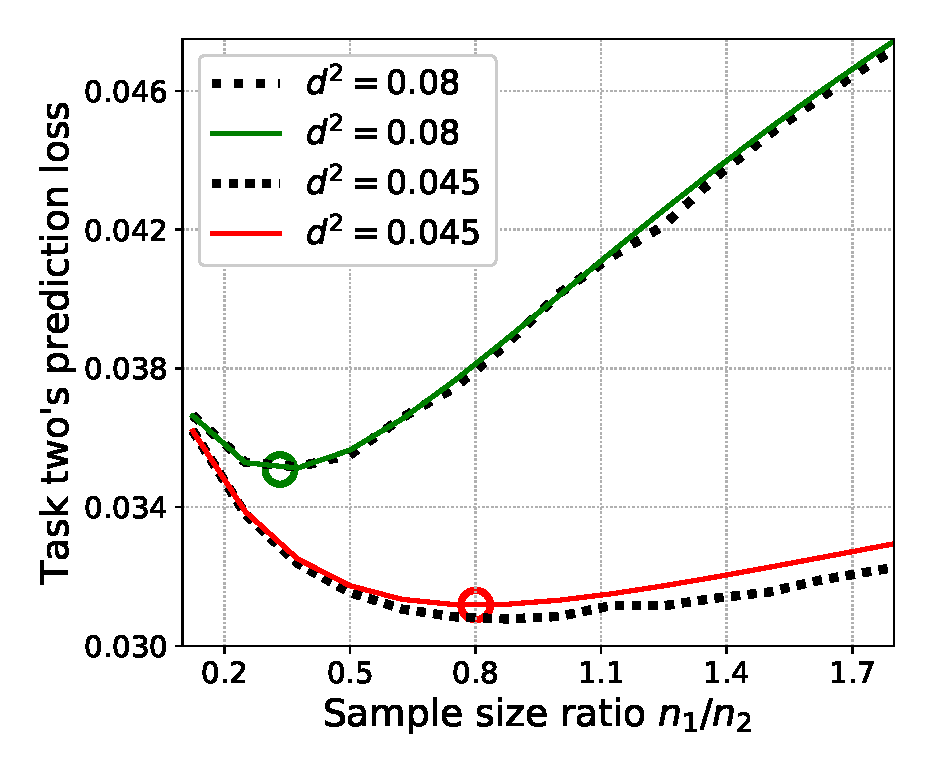
\includegraphics[width=0.98\textwidth]{figures/sample_ratio_several_d.eps}
		\caption{Example \ref{ex_sample_ratio}}
		\label{fig_size}
	\end{subfigure}\hfill
	\begin{subfigure}[b]{0.33\textwidth}
		\centering
		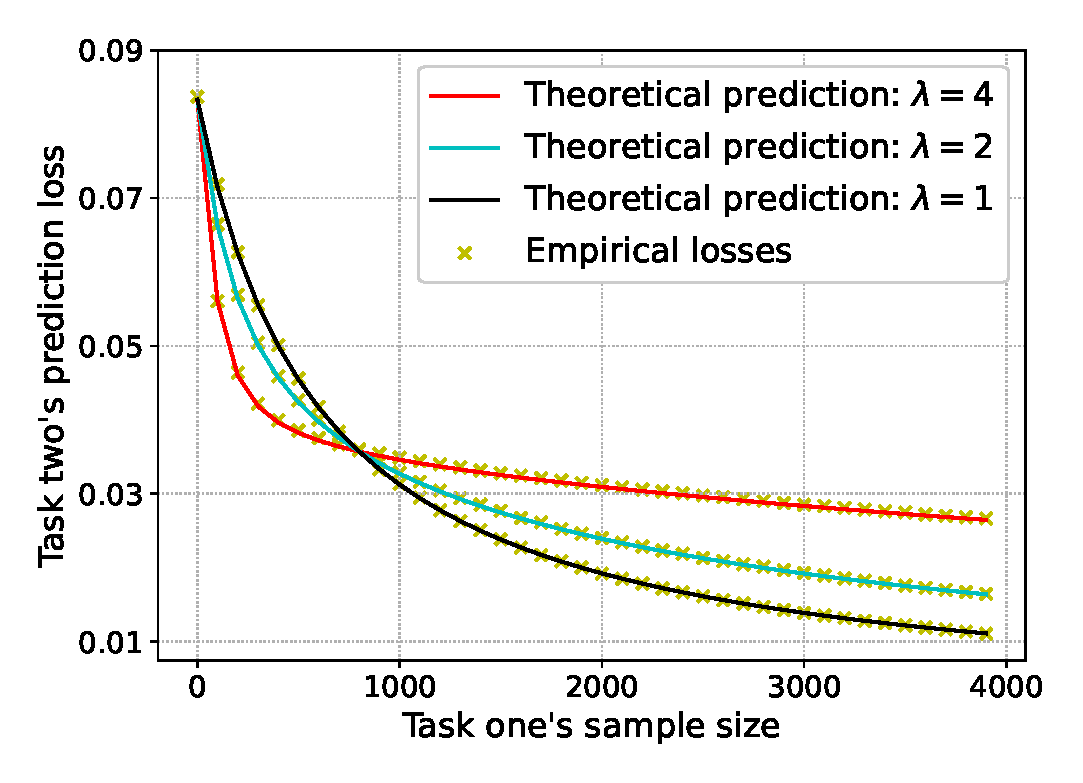
\includegraphics[width=0.98\textwidth]{figures/covariate_shift.eps}
		\caption{Example \ref{ex_covshift}}
		\label{fig_covariate}
	\end{subfigure}
	\caption{%Three takeaways of our theory in Section \ref{sec_insight}.
	Our estimated losses (solid line) match the empirical losses (dotted line) accurately under various settings in dimension $p = 200$.
	\textbf{Left.} Validating Example \ref{ex_same_cov} for ten tasks: the noise variance $\sigma^2$ is $1/4$.
	\textbf{Middle.} Validating Example \ref{ex_sample_ratio} for two tasks: we discover an interesting phenomena by fixing task two's sample size and increasing task one's sample size.
	Moreover, our result accurately predicts the critical point (marked in circle) of the loss curve.
%	Depending on how large the distance $d^2$ is, task two's prediction loss decreases initially before increasing again, or decreases monotonically.
	\textbf{Right.} We show how different levels of covariate shift affect hard parameter sharing when there is no bias.
	Having covariate shift increases task two's prediction loss when task two's sample size is smaller than task one. Otherwise, having covariate shift (surprisingly) decreases task two's prediction loss.}
	\label{fig_model_shift_phasetrans}
\end{figure*}



%Recall that  $U\Lambda V^\top$ is the singular value decomposition of $M$, %$\Lambda$ consists of the singular values of $M$, $V$ is an orthonormal matrix,
%It is not hard to verify that $(n_1 + n_2)\hat{\Sigma}^{-1}= (\Sigma^{(2)})^{-1/2} V W^{-1}V^\top (\Sigma^{(2)})^{-1/2}$ and .
Let $\mu=p^{-1}\sum_{i} \delta_{\sigma_i}$ denote the empirical spectral distribution of $W$, where the $\sigma_i$'s are the eigenvalues of $W$ and $\delta_{\sigma_i}$ is the point mass measure at $\sigma_i$. Then it is easy to see that the Stieltjes transform of $\mu$ is equal to
 \[ m_{\mu}(z) \define \frac{1}{p}\sum_{i=1}^p \frac{1}{\sigma_i - z}= p^{-1}\tr\left[(W-z\id)^{-1}\right]. \]
The above matrix $(W - z\id)^{-1}$ is known as $W$'s resolvent or Green's function.
%When $p$ goes to infinity, it is well-known that $m_{\mu}(z)$ converges to a fixed distribution governed by a set of self-consistent equations.
%These self-consistent equations give the asymptotic limit of the trace of $\hat{\Sigma}^{-1}$.
%The above approach applies when $\Sigma^{(2)}$ is isotropic in Theorem \ref{thm_main_RMT}.
%Since our goal is to show the limit of $\tr\left[ (Y - z\id)^{-1}V^{\top}{\Sigma^{(2)}}^{-1}V \right]$ as shown in equation \eqref{eigen2extra}, we study the  $(Y-z\id)^{-1}$.
%Compared to the Stieltjes transform, the resolvent also applies to random matrices.
We prove the convergence of $W$'s resolvent using the so-called ``local law'' with a sharp convergence rate \cite{isotropic,erdos2017dynamical,Anisotropic}. The complete proof is provided in Section \ref{appendix RMT}.
%Recent developments in the random matrix literature have shown the convergence of the resolvent matrix using the so-called ``local laws'' or ``deterministic equivalents'' (cf. \cite{Hachem2007deterministic,DS18}).

%For our purpose, we use a convenient linearization trick in linear algebra, that is, the SVD of a rectangular matrix $A$ is equivalent to the study of the eigendecomposition of the symmetric block matrix
%$$H(A):=\begin{pmatrix}0 & A \\ A^\top & 0\end{pmatrix},$$
%which is linear in $A$. This trick has been used in many random matrix literatures, such as \cite{Anisotropic, AEK_Gram, XYY_circular,DY20201}.



\section{Experiments}

\paragraph{A metric to determine when MTL performs better STL.}

\paragraph{When should we align task covariances in MTL.}
\begin{figure}
	\centering
	\includegraphics[width=0.5\textwidth]{figures/ratio_alignment_mr_sst_lstm.pdf}
	\caption{Covariate shift experiment.}
\end{figure}
\subsection{Further Studies on Text Classification Tasks}\label{sec_text}

Our results and simulations are all in the high-dimensional linear regression setting.
How well do they extend to other scenarios?
In this section, we conduct further studies on six text classification datasets.
Our datasets include a movie review sentiment dataset (MR) \cite{pang2005seeing}, a sentence subjectivity dataset (SUBJ) \cite{pang2004sentimental}, a customer reviews dataset (CR) \cite{hu2004mining}, a question type dataset (TREC) \cite{li2002learning}, an opinion polarity dataset (MPQA) \cite{wiebe2005annotating}, and the Stanford sentiment treebank (SST) dataset \cite{socher2013recursive}.
Our model consists of a word embedding layer with GloVe embeddings \cite{pennington2014glove} followed by a long-short term memory (LSTM) or a multi-layer perception (MLP) layer \cite{lei2018simple}.\footnote{For MLP, we apply an average pooling layer over word embeddings. For LSTM, we add a shared feature representation layer on top of word embeddings.}


\paragraph{Sample size ratio.}
First, we show that our observation in Figure \ref{fig_size} also occurs in the text classification tasks.
In Figure \ref{fig_ab_data}, we observe that for multiple example task pairs, increasing task one's sample size improves task two's prediction accuracy initially but hurts eventually.
On the $y$-axis, we plot task two's test accuracy using HPS, subtracted by its STL test accuracy.
We fix task two's sample size at $1000$ and increase task one's sample size from $100$ to $3000$.

These examples and Figure \ref{fig_size} suggest a natural progressive training schedule, where we add samples progressively until performance drops.
Concretely, here is one implementation of this idea.
\begin{itemize}
	\item We divide the training data into $S$ batches.
	We divide the training procedure into $S$ stages. During every stage, we progressively add one more data batch.
	\item During every stage, we train for $T$ epochs using only the $S$ batches. If the validation accuracy drops compared to the previous round's result or reaches the desired threshold $\tau$, we terminate.
\end{itemize}
If we apply this procedure to the settings of Figure \ref{fig_ab_data} and \ref{fig_size}, it will terminate once reaching the optimal sample ratio.
The advantage of this procedure is that it reduces the computational cost compared to standard round-robin training schedules.
For example, if the process terminates at 30\% of all batches, then SGD only passes over 30\% of its data, whereas standard round-robin training passes over 100\% of task one's data.


We evaluate the progressive training procedure on the six text classification datasets.
First, we conduct multi-task training over all the $15$ two-task pairs from the six datasets.
We focus on task two's test accuracy and set $\tau$ as task two's test accuracy obtained via the standard round-robin training schedule.
We include all of task two's data and progressively add task one's data using the procedure described above.
Since the prediction accuracy has been controlled the same, we compare the computational cost.
We find that when averaged over all the $15$ two-task pairs, this procedure requires only $45\%$ of the computational cost to reach the desired accuracy $\tau$ for task two.
Second, we conduct multi-task training on all six datasets jointly.
We extend our procedure to all six datasets. We include the data from all tasks except SST. For SST, we progressively add data similar to the above procedure.
We set $\tau$ to be the average test accuracy of all the six tasks obtained using standard round-robin training.
We find that adding samples progressively from SST requires less than $35\%$ of the computational cost to reach the same average test accuracy $\tau$.







\paragraph{Covariate shift.}
Recall from Example \ref{ex_covshift} that having covariate shifts worsens the variance (hence the loss) of hard parameter sharing when the sample ratio increases.
This highlights the need for correcting covariate shifts when the sample size ratio rises.
To this end, we study a covariance alignment procedure proposed in \citet{WZR20}, designed to correct covariate shifts.
The idea is to add an alignment module between the input and the shared module $B$.
This module is then trained together with $B$ and the output layers. We refer to \citet{WZR20} for more details about the procedure and the implementation.

We conduct multi-task training on all $15$ task pairs from the six datasets.
In Figure \ref{fig_ab_cov}, we measure the performance gains from performing covariance alignment vs. HPS.
To get a robust comparison, we average the improvements over the 15 task pairs.
The result shows that as the sample size ratio increases, performing covariance alignment provides more significant gains over HPS.
We fix task two's sample size at $1,000$, and increase task one's sample size from $1,000$ to $3,000$.





\begin{figure}%
	\begin{subfigure}[t]{0.5\textwidth}
		\centering
		\vspace{0pt}
		\includegraphics[width=0.8\textwidth]{figures/fig3a.pdf}
		\caption{HPS vs. STL}
		\label{fig_ab_data}
	\end{subfigure}\hfill
	\begin{subfigure}[t]{0.5\textwidth}
		\centering
		\vspace{0pt}
		\includegraphics[width=0.8\textwidth]{figures/fig3b.pdf}
		\caption{HPS vs. covariance alignment}
		\label{fig_ab_cov}
	\end{subfigure}
	\caption{Comparing hard parameter sharing (HPS) to single-task learning (STL) and a covariance alignment approach proposed by \citet{WZR20}:
	In Figure \ref{fig_ab_data}, we observe that for multiple task pairs, increasing task one's sample size improves task two's prediction accuracy initially, but hurts eventually -- a phenomenon similar  to Figure \ref{fig_size}.
	In Figure \ref{fig_ab_cov}, we observe that as task one's sample size increases, covariance alignment improves more over HPS.}
	\label{fig_text}
\end{figure}


\section{Conclusions}\label{sec_conclude}

Distribution shift is a fundamental challenge in applying transfer learning.
This work formulated a theoretical setup in which questions related to the transfer effect can be formally analyzed.
The setup can reproduce several interesting phenomena in the context of transfer learning.
Precise asympotics for the risk of a two-layer linear neural network are shown under various kinds of distribution shift.
Such analysis has led to a number of theoretical insights and practical implications for applying transfer learning to text classification tasks.

%We describe several open questions for future work.
%First, it would be interesting to tighten our estimate in Corollary \ref{cor_MTL_loss}, which would extend the observation in Figure \ref{fig_size} to small $n_1$.
%Second, it would be interesting to extend our result to classification problems such as logistic regression.
It is a very interesting question to derive the asymptotic limit under general covariate and model shift.
%This requires showing the limit of $\normFro{\big(({Z^{(1)}})^{\top} Z^{(1)} + {Z^{(2)}}^{\top} Z^{(2)}\big)^{-1} {Z^{(1)}}^{\top} Z^{(1)}}^2$ for two sample covariance matrices.
We remark that likely such a result will require studying the asymptotic distribution of the singular values of asymmetric matrices, which is technically challenging.
%FY: $+\id$ is very important and makes the problem very hard; otherwise the problem can be solved with current RMT methods.
%The eigenvalue distribution of this matrix, which has been obtained in \cite{Fmatrix}, might be helpful towards resolving this problem.
%but its singular values will follow a different distribution since the matrix is not symmetric.
 %might require new techniques beyond the current ones in random matrix theory .%\HZ{to add}.
Another interesting question is to study the impact of distribution shift in other settings such as logistic regression \cite{sur2019modern}.

%\begin{supplement}
%\textbf{Supplement to ``High-dimensional Asymptotics of Transferring from Different Domains in Linear Regression"}.
%In the Internet Appendix \cite{MTL_suppl}, we provide the proofs of the technical results in Sections \ref{sec_HPS}-\ref{sec_diff}, including Lemma \ref{lem_HPS_loss}, Theorem \ref{thm_many_tasks}, Theorem \ref{cor_MTL_loss}, Proposition \ref{lem_hat_v}, Theorem \ref{thm_main_RMT} and Proposition \ref{prop_main_RMT}.
%and give the technical proofs of the main theorems, Theorems \ref{thm_regularbm}, \ref{thm_twgram}, \ref{thm_twgraph} and  \ref{thm_twgraph_sparse}.
%\end{supplement}


\subsection*{Acknowledgements:}
Thanks to Edgar Dobriban, Vaggos Chatziafratis, Mayee Chen, and Ruoxuan Xiong for helpful discussions at various stages of this work.
HZ and WS's contributions were in part supported by the Wharton Dean's Fund for Postdoctoral Research.
We gratefully acknowledge the support of DARPA under Nos. FA86501827865 (SDH) and FA86501827882 (ASED); NIH under No. U54EB020405 (Mobilize), NSF under Nos. CCF1763315 (Beyond Sparsity), CCF1563078 (Volume to Velocity), and 1937301 (RTML); ONR under No. N000141712266 (Unifying Weak Supervision); the Moore Foundation, NXP, Xilinx, LETI-CEA, Intel, IBM, Microsoft, NEC, Toshiba, TSMC, ARM, Hitachi, BASF, Accenture, Ericsson, Qualcomm, Analog Devices, the Okawa Foundation, American Family Insurance, Google Cloud, Swiss Re, the HAI-AWS Cloud Credits for Research program, and members of the Stanford DAWN project: Teradata, Facebook, Google, Ant Financial, NEC, VMWare, and Infosys. The U.S. Government is authorized to reproduce and distribute reprints for Governmental purposes notwithstanding any copyright notation thereon. Any opinions, findings, and conclusions or recommendations expressed in this material are those of the authors and do not necessarily reflect the views, policies, or endorsements, either expressed or implied, of DARPA, NIH, ONR, or the U.S. Government.


\bibliographystyle{plainnat}
\bibliography{rf,ref_mtl}
\appendix


	\section{Proof of Lemma \ref{lem_error_same_cov}}\label{app_proof_error_same_cov}
	Next, we show that the concentration errors of $g_0(\cW), g_1(\cW), g_2(\cW)$ are all lower order terms compared to $\ex{g(\cW)}$.

	First, for $g_1(\cW)$, using Lemma \ref{largedeviation} in Appendix \ref{sec_maintools} and the fact that all moments of $\varepsilon_i$ exist, we obtain that for a sufficiently small constant $\e>0$, the following holds with high probability:
	\[ \text{for any } 1\le j \le t, |\inner{XB^{\star} \cW^{\top} (\cW\cW^{\top})^{-1}W_j - X\beta_j}{\varepsilon_j}| \le p^\e \sigma\|XB^{\star} \cW^{\top} (\cW\cW^{\top})^{-1}W_j - X\beta_j\|. \]
	%and
	%\begin{align*}  &|\inner{XB^{\star} \cW^{\top} (\cW\cW^{\top})^{-1}W_j - X\beta_j}{U_X U_X^{\top} \bigbrace{\varepsilon_i W_i^{\top}} (\cW\cW^{\top})^{-1} W_j }| \\
	%&\le p^\e \sigma |W_i^{\top} (\cW\cW^{\top})^{-1} W_j|\cdot \|U_X U_X^{\top}( {XB^{\star} \cW^{\top} (\cW\cW^{\top})^{-1}W_j - X\beta_j})\|
	%\end{align*}
	Applying the above estimates into $g_1(\cW)$, we get that
	\begin{align}
	  \abs{g_1(\cal W)}    &\le p^\e \sigma \sum_{j=1}^t \|  {XB^{\star} \cW^{\top} (\cW\cW^{\top})^{-1}W_j - X\beta_j}\| \nonumber \\
	&\le  p^\e \sigma \sum_{j=1}^t \bignorm{  \Sigma^{1/2}\left(B^{\star} \cW^{\top} (\cW\cW^{\top})^{-1}W_j - \beta_j\right)} \cdot \|Z\| \nonumber\\
	&\lesssim p^{1/2+\e} \sigma \sum_{j=1}^t \bignorm{  \Sigma_1^{1/2}\left(B^{\star} \cW^{\top} (\cW\cW^{\top})^{-1}W_j - \beta_j\right)} \nonumber\\
	& \le p^{1/2+\e} \bignorm{\Sigma^{1/2} B^{\star} (\cW^{\top} (\cW \cW^{\top})^{-1} \cW - \id_{t\times t})}^2 + t\sigma^2 p^{1/2+\e}.  \label{eq_est_g1}
	\end{align}
	In the second step, we use the fact that $X=Z\Sigma^{1/2}$.
	In the third step, we use equation \eqref{eq_isometric} to bound the operator norm $\|Z\|$ by $\OO(\sqrt{p})$.
	In the last step, we use the AM-GM inequality.

	Second, for $g_2(\cW)$, using Lemma \ref{largedeviation} in Appendix \ref{sec_maintools} and the fact that all moments of $\varepsilon_i$ exist, we obtain that for any $1\le i, j \le t$, the following holds with high probability:
	\begin{align*}
		\bigabs{\norm{\varepsilon_j}^2 - \ex{\norm{\varepsilon_j}^2}} &\le \sigma^2 p^{1/2+\e},\\
		%|\inner{U_X U_X^{\top} \bigbrace{\varepsilon_i W_i^{\top}} (\cW\cW^{\top})^{-1}W_j}{\varepsilon_j}|
		\abs{W_i^{\top} (\cW\cW^{\top})^{-1} W_j \cdot \bigbrace{\varepsilon_i^{\top} U_X U_X^{\top} \varepsilon_j}}
		&\le |W_i^{\top} (\cW\cW^{\top})^{-1}W_j| \cdot \sigma^2 p^{\e} \bigtr{(U_X U_X^{\top})^2}^{1/2} \le \sigma^2 p^{1/2+\e}
  % &\left|\left(1-\mathop{\mathbb{E}}_{\varepsilon_j} \right)\left[\inner{U_X U_X^{\top} \bigbrace{\varepsilon_j W_j^{\top}} (\cW\cW^{\top})^{-1}W_j}{\varepsilon_j}\right]\right| \le |W_j^{\top} (\cW\cW^{\top})^{-1}W_j| \cdot \sigma^2 p^{\e} \tr \left[(U_X U_X^{\top})^2\right]\le \sigma^2 p^{1/2+\e},\\
  % &\left|\left(1-\mathop{\mathbb{E}}_{\varepsilon_j} \right)\left[\inner{U_X U_X^{\top} \bigbrace{\varepsilon_j W_j^{\top}} (\cW\cW^{\top})^{-1}W_j}{U_X U_X^{\top} \bigbrace{\varepsilon_j W_j^{\top}} (\cW\cW^{\top})^{-1}W_j}\right]\right|\\
  % &\le |W_j^{\top} (\cW\cW^{\top})^{-1}W_j|^2 \cdot \sigma^2 p^{\e} \tr \left[(U_X U_X^{\top})^4\right]\le \sigma^2 p^{1/2+\e},
	\end{align*}
	Combining the above two inequalities together, we get that with high probability
	\begin{align}
		\left|g_2(\cal W)-\sigma^2(n\cdot t - p\cdot r)\right|=\left|g_2(\cal W)- \exarg{\varepsilon_1, \dots, \varepsilon_t} {g_2(\cal W)}\right| \lesssim \sigma^2 p^{1/2+\e}. \label{eq_est_g2}
	\end{align}

	Finally, for $g_0(\cW)$, denote by $v_j:= \Sigma^{1/2}\left(B^{\star} \cW^{\top} (\cW\cW^{\top})^{-1} W_j -  \beta_j\right)$, for any $j = 1,\dots,t$, we have that $g_0(\cal W)= \sum_{j=1}^t\left\|Z v_j \right\|^2$.
%	$$g_0(\cal W)= \sum_{j=1}^t\left\|Z v_j \right\|^2,\quad v_j:= \Sigma^{1/2}\left(B^{\star} \cW^{\top} (\cW\cW^{\top})^{-1} W_j -  \beta_j\right).$$
	Note that $Zv_j\in \R^n$ is a random vector with i.i.d. entries of mean zero, variance $\|v_j\|^2$, and finite fourth moment by \eqref{assmAhigh}.
	Hence by law of large numbers, we have that with high probability
	${\left\|Z v_j \right\|^2 } = { n \|v_j\|^2} \cdot (1+\oo(1))$,
	which implies that
	\begin{align}
		g_0(\cal W)=n \sum_{j=1}^t \|v_j\|^2 \cdot (1+\oo(1)) = n \bignorm{\Sigma^{1/2} B^{\star} (\cW^{\top} (\cW \cW^{\top})^{-1} \cW - \id_{t\times t})}^2 \cdot (1+\oo(1)). \label{eq_est_g0}
	\end{align}

	Combining equation \eqref{eq_est_g1}, \eqref{eq_est_g2}, and \eqref{eq_est_g0}, we obtain that with high probability
	\begin{align}
	g(\cal W)&= n \bignorm{\Sigma^{1/2} B^{\star} (\cW^{\top} (\cW \cW^{\top})^{-1} \cW - \id_{t\times t})}^2 \cdot (1+\oo(1)) + \sigma^2 (n\cdot t - p \cdot r)+\OO(\sigma^2 p^{1/2+\e}) \nonumber \\
	&=\ex{g(\cW)} \cdot (1+\oo(1)) + \OO(\sigma^2 p^{1/2+\e}). \label{eq_est_g}
	\end{align}

\section{Missing Proof of the Different Covariates Setting}\label{sec_maintools}

\subsection{Proof of the Bias and Variance Asymptotics}\label{appendix RMT}

We provide the proof of Theorem \ref{thm_main_RMT}.
We begin with a warm up analysis when the entries of $Z^{(1)}$ and $Z^{(2)}$ are drawn i.i.d. from an isotropic Gaussian distribution.
By the rotational invariance of the multivariate Gaussian distribution, we have that the entries of $Z^{(1)} U$ and $Z^{(2)}$ also follow an isotropic Gaussian distribution.
Hence it suffices to consider the following resolvent
 \begin{equation} \label{resolv Gauss1}
   G(z)= \left( {\begin{array}{*{20}c}
   { -z\id_{p} } & n^{-1/2}\Lambda (Z^{(1)})^\top & n^{-1/2} (Z^{(2)})^\top  \\
   {n^{-1/2} Z^{(1)} \Lambda  } & {-\id_{n_1}} & 0 \\
   {n^{-1/2} Z^{(2)}} & 0 & {-\id_{n_2}}
   \end{array}} \right)^{-1}.
 \end{equation}
We show how to derive the matrix limit $\Gi(z)$ and the self-consistent equation system \eqref{selfomega_a}.
We first introduce several notations.
Define the index sets
$$\cal I_0:=\llbracket 1,p\rrbracket, \quad  \cal I_1:=\llbracket p+1,p+n_1\rrbracket, \quad \cal I_2:=\llbracket p+n_1+1,p+n_1+n_2\rrbracket ,\quad \cal I:=\cal I_0\cup \cal I_1\cup \cal I_2  .$$
%We will consistently use the latin letters $i,j\in\sI_{0}$ and greek letters $\mu,\nu\in\sI_{1}\cup \sI_{2}$.
Correspondingly, the indices of the matrices $Z^{(1)}$ and $Z^{(2)}$ are labelled as
	\be\label{labelZ}
 Z^{(1)}= [Z^{(1)}_{\mu i}:i\in \mathcal I_0, \mu \in \mathcal I_1], \quad Z^{(2)}= [Z^{(2)}_{\nu i}:i\in \mathcal I_0, \nu \in \mathcal I_2].\ee
We will study the following partial traces of the resolve $G(z)$:
\be\label{defm}
\begin{split}
m(z) :=\frac1p\sum_{i\in \cal I_0} G_{ii}(z) ,\quad & m_0(z):=\frac1p\sum_{i\in \cal I_0} \lambda_i^2 G_{ii}(z),\\
 m_1(z):= \frac{1}{n_1}\sum_{\mu \in \cal I_1}G_{\mu\mu}(z) ,\quad & m_2(z):= \frac{1}{n_2}\sum_{\nu\in \cal I_2}G_{\nu\nu}(z).
\end{split}
\ee
To deal with the matrix inverse, we consider the following resolvent minors of $G(z)$.
\begin{definition}[Resolvent minors]\label{defn_Minor}
	Let $X \in \real^{(p + n_1 + n_2)\times (p + n_1 + n_2)}$ and $i = 1, 2, \dots, p + n_1 + n_2$.
	The minor of $X$ after removing the $i$-th row and column of $X$ is denoted by $X^{(i)} := [X_{a_1,a_2}:a_1, a_2 \in \mathcal I\setminus \{i\}]$ as a square matrix with dimension $p + n_1 + n_2 - 1$.
	For the indices of $X^{(i)}$, we use $X^{(i)}_{a_1, a_2}$ to denote $ X_{a_1, a_2}$ when $a_1$ and $a_2$ both not equal to $i$, and $X^{(i)}_{a_1, a_2}$ to be zero when $a_1 = i$ or $a_2 = i$.
	The resolvent minor of $G(z)$ after removing the $i$-th row and column is defined as
	\begin{align*}
		G^{(i)}(z) := \left[ \left( {\begin{array}{*{20}c}
		  { -z\id_{p} } & n^{-1/2}\Lambda (Z^{(1)})^\top & n^{-1/2} (Z^{(2)})^\top  \\
      {n^{-1/2} Z^{(1)} \Lambda  } & {-\id_{n_1}} & 0 \\
			{n^{-1/2} Z^{(2)}} & 0 & {-\id_{n_2}}
    \end{array}} \right)^{(i)}\right]^{-1}.
	\end{align*}
\end{definition}
As a remark, we denote the partial traces $m^{(i)}(z)$, $m_0^{(i)}(z)$, $m_1^{(i)}(z)$, and $m_2^{(i)}(z)$ by replacing $G(z)$ with $G(z)^{(i)}$ in equation \eqref{defm}.

\paragraph{Self-consistent equations.}
We briefly describe the ideas for deriving the equation set \eqref{selfomega_a}.
A complete full can be found in Lemma \ref{lemm_selfcons_weak}.
We show that with high probability, the following equations hold approximately:
\be\label{approximate m1m2}
\begin{split}
& m_1^{-1}(z) = -1+ \frac{1}{n} \sum_{i=1}^p \frac{\lambda_i^2 }{ z +\lambda_i^2 \frac{\rho_1}{\rho_1+\rho_2} m_1(z) +  \frac{\rho_2}{\rho_1+\rho_2}m_2(z)+\oo(1)}+ \oo(1),\\
& m_2^{-1}(z) = -1+\frac{1}{n} \sum_{i=1}^p \frac{1}{ z +\lambda_i^2 \frac{\rho_1}{\rho_1+\rho_2} m_1(z) +  \frac{\rho_2}{\rho_1+\rho_2}m_2(z)+\oo(1)}  + \oo(1).
\end{split}
\ee
These are the self-consistent equations that we stated in equation \eqref{selfomega_a}.
More precisely, we have that $m_1(z)$ is approximately equal to $-\frac{n_1 + n_2}{n_2} a_1(z) $ and $m_2(z)$ is approximately equal to $-\frac{n_1 + n_2}{n_2} a_2(z)$.

The core idea is to study $G(z)$ using the Schur complement formula.
First, we consider the diagonal entries of $G(z)$ for each block in $\cal I_0$, $\cal I_1$, and $\cal I_2$.
For any $i$ in $\cal I_0$, any $\mu$ in $\cal I_1$, and any $\nu$ in $\cal I_2$, we have that
\begin{align*}
	&G_{i,i}^{-1}(z) = -z - \frac{\lambda_i^2}{n} \sum_{\mu,\nu\in \mathcal I_1} Z^{(1)}_{\mu i}Z^{(1)}_{\nu i}G^{\left( i \right)}_{\mu,\nu}(z) - \frac{1}{n} \sum_{\mu,\nu\in \mathcal I_2} Z^{(2)}_{\mu i}Z^{(2)}_{\nu i} G^{\left( i \right)}_{\mu,\nu}(z) -\frac{2\lambda_i}{n} \sum_{\mu\in \cal I_1,\nu\in \mathcal I_2} Z^{(1)}_{\mu i}Z^{(2)}_{\nu i}G^{\left( i \right)}_{\mu,\nu}(z) \\
	&G_{\mu,\mu}^{-1}(z) =  - 1 - \frac{1}{n} \sum_{i,j\in \mathcal I_0}\lambda_i \lambda_j Z^{(1)}_{\mu i}Z^{(1)}_{\mu j} G^{\left(\mu\right)}_{ij}(z) \\
	&G_{\nu,\nu}^{-1}(z) =  - 1 - \frac{1}{n} \sum_{i,j\in \mathcal I_0}  Z^{(2)}_{\nu i}Z^{(2)}_{\nu j}  G^{\left(\nu\right)}_{i,j}(z).
\end{align*}
For the first equation, we expand the Schur complement formula $G_{ii}^{-1}(z) = -z - H_i G^{(i)}(z) H_{i}^\top$, where $H_i$ is the $i$-th row of $H$ with the $(i,i)$-th entry removed.
The second and third equation follow by similar calculations.

%\be\label{approx m12 add}
%(m_1,m_2) =\left(-\frac{\rho_1+\rho_2}{\rho_1}a_{1}(z),-\frac{\rho_1+\rho_2}{\rho_2}a_{2}(z)\right)+\oo(1) \quad \text{with overwhelming probability. }
%\ee

Next, we apply standard concentration bounds to simplify the above results.
For $G^{-1}_{i, i}(z)$, recall that the resolvent minor $G^{(i)}$ is defined such that it is independent of the $i$-th row and column of $Z^{(1)}$ and $Z^{(2)}$.
Hence by standard concentration inequalities, we have that the cross terms are approximately zero.
%is approximately equal to the expectation over $\{Z^{(1)}_{\mu i}: \mu \in \cal I_1 \}\cup \{Z^{(2)}_{\nu i}: \nu \in \cal I_2\}$.
As shown in Lemma \ref{lemm_selfcons_weak}, we have that with high probability the following holds
\begin{align*}
	G_{i,i}^{-1}(z) &= -z - \frac{\lambda_i^2}{n} \sum_{\mu \in \mathcal I_1}  G^{\left( i \right)}_{\mu\mu} - \frac{1}{n} \sum_{\mu\in \mathcal I_2} G^{\left( i \right)}_{\mu\mu} +\oo(1) \\
	&= - z - \frac{\lambda_i^2 \cdot n_1}{n_1 + n_2} m_1^{(i)}(z)-  \frac{n_2}{n_1 + n_2} m_2^{(i)}(z)+\oo(1)
\end{align*}
by our definition of the partial traces $m_1^{(i)}(z)$ and $m_2^{(i)}(z)$ with respect to the resolvent minor $G^{(i)}(z)$.
Since we removed only one column and one row from $H(z)$, $m_1^{(i)}(z)$ and $m_2^{(i)}(z)$ should be approximately equal to $m_1(z)$ and $m_2(z)$.
Hence we obtain that
\begin{align}\label{1self_Gii}
	G_{i,i}(z)  = -\left(z + \frac{\lambda_i^2 \cdot n_1}{n_1 + n_2} m_1(z) +  \frac{n_2}{n_1 + n_2} m_2(z) + \oo(1)\right)^{-1}.
\end{align}
For the other two blocks $\cal I_1$ and $\cal I_2$, using similar ideas we have that the following holds with high probability
\begin{align*}
	G_{\mu,\mu}(z) &= -\left(1+\frac{p}{n_1 + n_2} m_0(z) + \oo(1)\right)^{-1} \\
	G_{\nu,\nu}(z) &= -\left(1+\frac{p}{n_1 + n_2} m(z) + \oo(1)\right)^{-1}.
\end{align*}
By averaging the above results over $\mu \in \cal I_1$ and $\nu \in \cal I_2$, we obtain that with high probability
\begin{align*}
	m_1(z) &= \frac{1}{n_1}\sum_{\mu \in \cal I_1}G_{\mu,\mu}(z) = -\left(1+\frac{p}{n_1 + n_2} m_0(z) + \oo(1)\right)^{-1} \\
	m_2(z) &= \frac{1}{n_2}\sum_{\nu \in \cal I_2}G_{\nu,\nu}(z) = -\left(1+\frac{p}{n_1 + n_2} m(z) + \oo(1)\right)^{-1}.
\end{align*}
Furthermore, we obtain that for $\mu \in \cal I_1$ and $\nu\in \cal I_2$, with high probability
$G_{\mu,\mu}(z) = m_1(z) +\oo(1)$ and $G_{\nu, \nu}(z) = m_2+\oo(1)$.
In other words, both block matrices within $\cal I_1$ and $\cal I_2$ are approximately a scaling of the identity matrix.
The above results for $m_1(z)$ and $m_2(z)$ imply that
\begin{align*}
	m_1^{-1}(z) = -1- \frac{1}{n} \sum_{i=1}^p \lambda_i^2 G_{i,i}(z)+ \oo(1) \\
	m_2^{-1}(z) = -1- \frac{1}{n} \sum_{i=1}^p G_{i,i}(z)  + \oo(1).
\end{align*}
where we used the definition of $m(z)$ and $m_0(z)$.
By applying equation \eqref{1self_Gii} for $G_{i, i}(z)$, we obtain the self-consistent equations \ref{approximate m1m2}.
In Lemma \ref{lem_stabw}, we show that the self-consistent equations are stable, that is, a small perturbation of the equations leads to a small perturbation of the solution.


Finally, we derive the matrix limit $\Gi(z)$.
Inserting the approximate identity \eqref{approx m12 add} into equations \eqref{1self_Gii} and \eqref{2.5self_Gmu}, we get that for  $i \in \cal I_0$, $\mu \in \cal I_1$ and $\nu\in \cal I_2$,
$$G_{ii}(z)=(-z +\lambda_i^2 a_{1}(z) + a_2(z)+\oo(1)^{-1},\quad G_{\mu\mu}=-\frac{\rho_1+\rho_2}{\rho_1}a_{1}(z)+\oo(1),\quad G_{\nu\nu}=-\frac{\rho_1+\rho_2}{\rho_2}a_{2}(z)+\oo(1),$$
with overwhelming probability. These explain the diagonal entries of $\Gi$ in equation \eqref{defn_piw}. For the off-diagonal entries, they are close to zero due to concentration. For example, for $i\ne j\in \cal I_1$, by Schur complement formula in equation (\ref{resolvent3}), we have
$$G_{ij}=-G_{ii}\Big({\lambda_i}{n^{-1/2}}\sum_{\mu \in \cal I_1} Z^{(1)}_{\mu i} G^{(i)}_{\mu j} + {n^{-1/2}}\sum_{\mu \in \cal I_2} Z^{(2)}_{\mu i} G^{(i)}_{\mu j} \Big).$$
Using Lemma \ref{largedeviation}, we can show that $n^{-1/2}\sum_{\mu \in \cal I_1} Z^{(1)}_{\mu i} G^{(i)}_{\mu j}$ and $n^{-1/2}\sum_{\mu \in \cal I_2} Z^{(2)}_{\mu i} G^{(i)}_{\mu j}$ are both close to zero. The other off-diagonal entries can be bounded in the same way. The bound on the off-diagonal entries will be proved rigorously in Lemma \ref{Z_lemma}.


\paragraph{Notations.}
We say an event $\Xi$ holds with overwhelming probability if for any constant $D>0$, $\mathbb P(\Xi)\ge 1- n^{-D}$ for large enough $n$. Moreover, we say $\Xi$ holds with overwhelming probability in an event $\Omega$ if for any constant $D>0$, $\mathbb P(\Omega\setminus \Xi)\le n^{-D}$ for large enough $n$.
We frequently use the following notion of stochastic domination, which was first introduced in \cite{Average_fluc} and subsequently used in many works on random matrix theory.
%It greatly simplifies the presentation of the results and their proofs by systematizing statements of the form ``$\xi$ is bounded by $\zeta$ with overwhelming probability up to a small power of $n$".

\begin{definition}[Stochastic domination]\label{stoch_domination}
%\begin{itemize}
%\item[(i)]
Let $\xi\equiv \xi^{(n)}$ and $\zeta\equiv \zeta^{(n)}$ be two $n$-dependent random variables.
\HZ{what is $n$-dependent rv?}
We say $\xi$ is stochastically dominated by $\zeta$, denoted by $\xi\prec \zeta$ or $\xi=\OO_\prec(\zeta)$, if for any (small) constant $\e>0$ and (large) constant $D>0$
\[ \bbP\left(|\xi| >n^\e |\zeta|\right)\le n^{-D}, \]
for large enough $n\ge n_0(\e, D)$. Moreover, if $\xi$ and $\zeta$ depend on a parameter $u$, then we say $\xi$ is stochastically dominated by $\zeta$ uniformly in $u\in \cal U$,  if for any constants $\e,D>0$,
\[\sup_{u\in \cal U}\bbP\left(|\xi(u)|>n^\e |\zeta(u)|\right)\le n^{-D}, \]
for large enough $n\ge n_0(\e, D)$.
%\item[(ii)]
%\end{itemize}
%(i) Let
%\[\xi=\left(\xi^{(n)}(u):n\in\bbN, u\in U^{(n)}\right),\hskip 10pt \zeta=\left(\zeta^{(n)}(u):n\in\bbN, u\in U^{(n)}\right)\]
%be two families of nonnegative random variables, where $U^{(n)}$ is a possibly $n$-dependent parameter set. We say $\xi$ is stochastically dominated by $\zeta$, uniformly in $u$, if for any fixed (small) $\epsilon>0$ and (large) $D>0$,
%\[\sup_{u\in U^{(n)}}\bbP\left[\xi^{(n)}(u)>n^\epsilon\zeta^{(n)}(u)\right]\le n^{-D}\]
%for large enough $n\ge n_0(\epsilon, D)$, and we shall use the notation $\xi\prec\zeta$.
%%Throughout this paper, the stochastic domination will always be uniform in all parameters that are not explicitly fixed (such as matrix indices, and $z$ that takes values in some compact set).
%%Note that $N_0(\epsilon, D)$ may depend on quantities that are explicitly constant, such as $\tau$ in Assumption \ref{assm_big1} and equation \eqref{assm_gap}.
%If for some complex family $\xi$ we have $|\xi|\prec\zeta$, then we will also write $\xi \prec \zeta$ or $\xi=\OO_\prec(\zeta)$.
%\item[(ii)]
%(ii) We extend the definition of $\OO_\prec(\cdot)$ to matrices in the weak operator sense as follows. Let $A$ be a family of random matrices and $\zeta$ be a family of nonnegative random variables. Then $A=O_\prec(\zeta)$ means that $\left|\left\langle\mathbf v, A\mathbf w\right\rangle\right|\prec\zeta \| \mathbf v\|_2 \|\mathbf w\|_2 $ uniformly in any deterministic vectors $\mathbf v$ and $\mathbf w$. Here and throughout the following, whenever we say ``uniformly in any deterministic vectors", we mean that ``uniformly in any deterministic vectors belonging to a set of cardinality $N^{\OO(1)}$".
%\item[(iv)]
%\end{itemize}
\end{definition}

For example, we say that $\xi$ is stochastically dominated by $\zeta$ with overwhelming probability if $\zeta$ is greater than $\xi$ up to a small power of $n^{\e}$.
Since we allow an $n^\e$ factor in the definition of stochastic domination, we have the seemingly strange inequality $(\log n)^C\prec 1$ for any constant $C>0$.
As another example, given a random variable $\xi$, if its moments exist up to any order, then we have $|\xi|\prec 1$. In fact, for any constants $\e, D>0$, by Markov's inequality we have
$$ \P(|\xi|\ge n^{\e})\le n^{-k\e}{\E |\xi|^k}\le n^{-D},$$
if we choose $k$ large enough such that $k\e>D$. As a special case, we have $|\xi|\prec 1$ for a Gaussian random variable $\xi$ with unit variance.

%\HZ{Why is this below part of the def. of stochastic domination?}


In this section, we shall prove a more fundamental random matrix result in a little more general setting than the one in Section \todo{add reference}; see Theorem \ref{LEM_SMALL} below. %\ref{sec_prelim}.
 Then Theorem \ref{thm_main_RMT} will follow from this result as immediate corollaries. We first state the exact assumptions needed for our purpose.

%We summarize our basic assumptions here for future reference. %Note that this assumption is in accordance with the assumptions of Lemma \ref{lem_cov_shift} and Lemma \ref{lem_cov_derivative}, except that we rescale the entries of $Z^{(1)}$ and $Z^{(2)}$ by $n^{-1/2}$. %and allow $\rho_1$ to be smaller than 1.
\begin{assumption}\label{assm_big1}
As in Section \todo{add reference}, we consider random matrices $X^{(1)}=Z^{(1)}\Sigma_1^{1/2}$ and $X^{(2)}=Z^{(2)}\Sigma_2^{1/2}$, where $Z^{(1)}$ and $Z^{(2)}$ are independent $n_1\times p$ and $n_2\times p$ random matrices with i.i.d. entries of zero mean and unit variance. Recall that $\rho_1= n_1/p$ and $\rho_2=n_2/p$. We assume that for a small constant $0<\tau<1$,
%\HZ{We have defined $\rho_1,\rho_2$ already in sec 2. Consider using ``Recall that $\rho_1 =, \rho_2 =$.''}
\be\label{assm2}
0\le \rho_1 \le \tau^{-1}, \quad 1+\tau \le \rho_{2} \le \tau^{-1}.
\ee
Recall that the singular value decomposition of $M = \Sig_1^{1/2} \Sig_2^{-1/2}$ is $U \Lambda V^{\top}$. We assume that
\begin{equation}\label{assm32}
\tau \le \lambda_p \le \lambda_1 \le \tau^{-1} .%, \quad \max\left\{\pi_A^{(n)}([0,\tau]), \pi_B^{(n)}([0,\tau])\right\} \le 1 - \tau .
\end{equation}
Finally, recalling the notations in equation \eqref{labelZ}, we assume that $Z^{(1)}$ and $Z^{(2)}$ satisfy
\begin{equation}
n^{-1/2}\max_{i\in \cal I_0,\mu \in \cal I_1}\vert Z^{(1)}_{\mu i}\vert \prec q,\quad n^{-1/2}\max_{i\in \cal I_0,\nu \in \cal I_2}\vert Z^{(2)}_{\nu i}\vert \prec q, \label{eq_support}
\end{equation}
for some deterministic parameter $q$ satisfying $ n^{-{1}/{2}} \leq q \leq n^{- \tau} $ for a small constant $\tau>0$.
%Here we recall the notations in \eqref{labelZ}.
 %and (\ref{assm2}). We assume that $T$ is an $M\times M$ deterministic diagonal matrix satisfying (\ref{simple_assumption}) and (\ref{assm3}).
\end{assumption}
%\HZ{This is restating what's stated above again. Remove redundant statements (unless there's something critical missing in Sec 2).} [\cor FY: The setting in sec 1 is too vague for the purpose of this section in the sense that it is hard to find the exact properties we need. In this section, I want to state rigorous statements with a reference to an exact assumption. Moreover, the above assumption contains more.\nc]


%\begin{remark}
%The lower bound $\rho_2\ge 1+\tau$ in equation \eqref{assm2} is to ensure that the sample covariance matrix $(X^{(2)})^\top X^{(2)}$ is non-singular with overwhelming probability. Moreover, we have allowed that $\rho_1=0$, because we want to state a general result that also covers the special case with no source task.
%\end{remark}


Whenever the estimates in equation \eqref{eq_support} hold, we say $n^{-1/2}Z^{(1)}$ and $n^{-1/2}Z^{(2)}$ satisfy the {\it{bounded support condition}} with $q$, or $n^{-1/2}Z^{(1)}$ and $n^{-1/2}Z^{(2)}$ have support $q$.
%\begin{definition}\label{defn_support}
%We say a (rescaled) random matrix $\cal M$ satisfies the {\it{bounded support condition}} with $q$, if
%\begin{equation}
%\max_{i,j}\vert \cal M_{ij}\vert \prec q. \label{eq_support}
%\end{equation}
%%Here $q\equiv q(n)$ is a deterministic parameter and usually satisfies $ n^{-{1}/{2}} \leq q \leq n^{- \phi} $ for some (small) constant $\phi>0$.
%Whenever (\ref{eq_support}) holds, we say that $M$ has support $q$.
%%Moreover, if the entries of $X$ satisfy (\ref{size_condition}), then $X$ trivially satisfies the bounded support condition with $q=N^{-\phi}$.
%\end{definition}
%\begin{example}
%\todo{Talk about the Gaussian case and Bernoulli case.}
As shown in the example above, if the entries of $Z^{(1)}$ have finite moments up to any order, %as in equation \eqref{assmAhigh},
then $n^{-1/2}Z^{(1)}$ has bounded support $n^{-1/2}$. More generally, if the entries of $Z^{(1)}$ have finite $\varphi$-th moment as in \eqref{assmAhigh}, then using Markov's inequality and a simple union bound we get that
\be\label{Ptrunc}
\P\left(n^{-1/2}\max_{i,\mu}|(Z^{(1)})_{\mu i}|\ge (\log n) n^{-\frac{\varphi-4}{2\varphi}}\right)=\OO((\log n)^{-\varphi}).\ee
In other words, $n^{-1/2}Z^{(1)}$ has bounded support $q=n^{-\frac{\varphi-4}{2\varphi}}$ on a event with probability $1-\oo(1)$. This leads to the exponent $\frac{\varphi-4}{2\varphi}$ in Fact \ref{lem_minv}. %This fact will be used in the proof of Corollary \ref{main_cor} below.
The above discussion shows that the bounded support condition provides great flexibility in dealing with finite moment conditions.
%\end{example}



%Recall that $n:=n_1+n_2$, which is the total number of data in the two tasks.
%Before giving the main proof, we first introduce some notations and tools.
%Following the notations in \cite{EKYY,EKYY1}, we will use the following definition to characterize events of overwhelming probability.
%
%\begin{definition}[overwhelming probability event] \label{high_prob}
%Define
%\begin{equation}\label{def_phi}
%\varphi:=(\log N)^{\log \log N}.
%\end{equation}
%We say that an $N$-dependent event $\Omega$ holds with {\it{$\xi$-overwhelming probability}} if there exist constant $c,C>0$ independent of $N$, such that
%\begin{equation}
%\mathbb{P}(\Omega) \geq 1-N^{C} \exp(- c\varphi^{\xi}),  \label{D25}
%\end{equation}
%for all sufficiently large $N$. For simplicity, for the case $\xi=1$, we just say {\it{overwhelming probability}}. Note that if (\ref{D25}) holds, then $\mathbb P(\Omega) \ge 1 - \exp(-c'\varphi^{\xi})$ for any constant $0\le c' <c$.
%\end{definition}
%\begin{remark}
%For any $c, C>0$, there exists a $0< c^{\prime}<c$, such that $N^{C} \exp(-c \varphi^{\xi}) \leq \exp(-c^{\prime} \varphi^{\xi})$. Hence, if
%\begin{equation}
%\mathbb{P}(\Omega) \geq 1- \exp(-c \varphi^{\xi})
%\end{equation}
%$\Omega$ is also a $\xi$-overwhelming probability event.
%\end{remark}


\subsection{Limit of the Resolvent}\label{sec pf RMTlemma}

We now state the main random matrix result---Theorem \ref{main_cor}---which gives an almost optimal estimate on the resolvent $G(z)$ of $H$. It is conventionally called the {\it anisotropic local law} \cite{Anisotropic}. We define a domain of the spectral parameter $z$ as
\begin{equation}
\mathbf D:= \left\{z=E+ \ii \eta \in \C_+: |z|\le (\log n)^{-1} \right\}. \label{SSET1}
\end{equation}

\begin{theorem}\label{main_cor}
In the setting of Theorem \ref{thm_main_RMT}, let $q$ be equal to $n^{-\frac{\varphi - 4}{2\varphi}}$.
We have that the resolvent $G(z)$ converges to the matrix limit $\Gi(z)$:
for any deterministic unit vectors $\mathbf u, \mathbf v \in \mathbb R^{p+n_1+n_2}$, the following estimate \begin{equation}\label{aniso_law}
	\max_{z\in \mathbf D}\left| \mathbf u^\top (G(z)-\Gi(z)) \mathbf v \right|  \prec  q
\end{equation}
holds on the high probability event
\be\label{one_event}\left\{ \max_{1\le i\le n_1, 1\le j \le p}|Z^{(1)}_{i j}| \le (\log n) n^{\frac{2}{\varphi}}, \ \max_{1\le i\le n_2, 1\le j \le p}|Z^{(2)}_{i j}|\le (\log n) n^{\frac{2}{\varphi}} \right\}.\ee
\end{theorem}

The above result can be derived using the following lemma, which holds under a more general bounded support assumption on the random matrices.

\begin{lemma} \label{LEM_SMALL} %
In the setting of Theorem \ref{main_cor}, assume that $Z^{(1)}$ and $Z^{(2)}$ satisfy the bounded support condition \eqref{eq_support} with $Q=\sqrt{n}q = n^{ \frac{2}{\varphi}}$.
Then we have that the anisotropic local law in equation \eqref{aniso_law} holds 
for any deterministic unit vectors $\mathbf u, \mathbf v \in \mathbb R^{p+n_1+n_2}$.
\end{lemma}

\begin{remark}
The reason why we say the bounded support assumption is more general is because it provides greater flexibility in dealing with bounded moments. For example, we can also replace equation \eqref{Ptrunc} with
\begin{align*}
	\P\left(\max_{1\le i\le n, 1\le j \le p}|Z_{i j}|\ge n^{\frac{2}{\varphi}+\delta}\right) = \OO(  n^{-\varphi \delta}) 
	\end{align*}
	for a small constant $\delta>0$. Hence we can replace event \eqref{one_event} with 
	\be\nonumber \left\{ \max_{1\le i\le n, 1\le j \le p}|Z^{(1)}_{i j}| \le n^{\frac{2}{\varphi}+\delta}, \ \max_{1\le i\le n, 1\le j \le p}|Z^{(2)}_{i j}|\le   n^{\frac{2}{\varphi}+\delta} \right\},\ee
	which holds with higher probability. But on this event we need to take a larger $q=n^{-\frac{\varphi - 4}{2\varphi}+\delta}$, which means a worse convergence rate. In general, with Lemma \ref{LEM_SMALL} one can determine the most suitable trade-off between probability and convergence rate depending on one's need.
\end{remark}

Using the above result, we prove Theorem \ref{main_cor} using a simple cutoff argument.
\begin{proof}[Proof of Theorem \ref{main_cor}]%
We introduce the truncated matrices $\wt Z^{(1)}$ and $\wt Z^{(2)}$ with entries
$$ \wt Z^{(1)}_{\mu i}:= \mathbf 1\left( n^{-1/2}|Z^{(1)}_{\mu i}|\le q \log n \right)\cdot Z^{(1)}_{\mu i}, \quad \wt Z^{(2)}_{\nu i}:= \mathbf 1\left( n^{-1/2}|Z^{(2)}_{\nu i}|\le q \log n \right)\cdot Z^{(2)}_{\nu i}, $$
for $q= n^{-\frac{\varphi - 4}{2\varphi}}$. By equation \eqref{Ptrunc}, 
we have
\begin{equation}\label{XneX}
\mathbb P(\wt Z^{(1)} = Z^{(1)},  \wt Z^{(2)} = Z^{(2)}) =1-\OO ( (\log n)^{-\varphi}).
\end{equation}
By definition, we have 
\be\label{EwtZ}
\begin{split}
\E  \wt  Z^{(1)}_{\mu i} &= - \mathbb E \left[ \mathbf 1\left( |Z^{(1)}_{\mu i}|> qn^{1/2} \log n \right)Z^{(1)}_{\mu i}\right] ,\\ 
\E  |\wt  Z^{(1)}_{\mu i}|^2 &= 1 - \mathbb E \left[ \mathbf 1\left( |Z^{(1)}_{\mu i}|> qn^{1/2} \log n \right)|Z^{(1)}_{\mu i}|^2\right] .
\end{split}
\ee
Using the formula for expectation in terms of the tail probabilities, we can check that
\begin{align*}
&  \mathbb E \left| \mathbf 1\left( |Z^{(1)}_{\mu i}|> q n^{1/2}\log n \right)Z^{(1)}_{\mu i}\right| \\
= &\int_0^\infty \P\left( \left| \mathbf 1\left(  |Z^{(1)}_{\mu i}|> q n^{1/2}\log n \right)Z^{(1)}_{\mu i}\right| > s\right)\dd s \\
 = &\int_0^{qn^{1/2}\log n}\P\left( |Z^{(1)}_{\mu i}|> q  n^{1/2}\log n \right)\dd s +\int_{qn^{1/2}\log n}^\infty \P\left(|Z^{(1)}_{\mu i}| > s\right)\dd s  \\
\lesssim &\int_0^{qn^{1/2}\log n}\left(q  n^{1/2}\log n \right)^{-\varphi}\dd s +\int_{qn^{1/2}\log n}^\infty s^{-\varphi}\dd s \le n^{-2(\varphi-1)/\varphi},
\end{align*}
where in the third step we used the finite $\varphi$-th moment condition of $Z_{\mu i}^{(1)}$ %
and Markov's inequality. Similarly, we can obtain that
\begin{align*}
&  \mathbb E \left| \mathbf 1\left( |Z^{(1)}_{\mu i}|> qn^{1/2} \log n \right)Z^{(1)}_{\mu i}\right|^2 \\
= & 2\int_0^\infty s \P\left( \left| \mathbf 1\left( |Z^{(1)}_{\mu i}|> q n^{1/2}\log n \right)Z^{(1)}_{\mu i}\right| > s\right)\dd s \\
= & 2\int_0^{qn^{1/2}\log n} s \P\left( |Z^{(1)}_{\mu i}|> q  n^{1/2}\log n \right)\dd s +2\int_{qn^{1/2}\log n}^\infty s\P\left(|Z^{(1)}_{\mu i}| > s\right)\dd s  \\
\lesssim & \int_0^{qn^{1/2}\log n}s\left(q  n^{1/2}\log n \right)^{-\varphi}\dd s +\int_{qn^{1/2}\log n}^\infty s^{-\varphi+1}\dd s \le n^{-2(\varphi-2)/\varphi}.
\end{align*}
Plugging the above two estimates into equation \eqref{EwtZ} and using $\varphi>4$, we get that
\be\label{meanshif}
|\mathbb E  \wt  Z^{(1)}_{\mu i}| =\OO(n^{-3/2}), \quad  \mathbb E |\wt  Z^{(1)}_{\mu i}|^2 =1+ \OO(n^{-1}).
\ee
From the first estimate in equation \eqref{meanshif}, we can also get a bound on the operator norm:
\be\label{EZ norm}\|\E \wt Z^{(1)}\|=\OO(n^{-1/2}) .
\ee
Similar estimates also hold for $\wt Z^{(2)}$. 
Then we can centralize and rescale $\wt Z^{(1)}$ and $\wt Z^{(2)}$ as
$$ \wh Z^{(1)} :=\frac{\wt Z^{(1)} - \E \wt Z^{(1)} }{\left(\E|\wt Z^{(1)}_{\mu i}|^2\right)^{1/2}},\quad \wh Z^{(2)} :=\frac{\wt Z^{(2)} - \E \wt Z^{(2)} }{\left(\E|\wt Z^{(2)}_{\mu i}|^2\right)^{1/2}}.$$ 
Now $\wh Z^{(1)}$ and $\wh Z^{(2)}$ satisfy the assumptions of Lemma \ref{LEM_SMALL} with bounded support $\sqrt{n}q = n^{ \frac{2}{\varphi}}$, so we get that %
\be\label{GwhZZ}\left| \mathbf u^\top (G(\wh Z^{(1)},\wh Z^{(2)},z)-\Gi(z)) \mathbf v \right|  \prec  q,\ee
where $G(\wh Z^{(1)},\wh Z^{(2)},z)$ is defined in the same way as $G(z)$, but with $(Z^{(1)}, Z^{(2)})$ replaced by $(\wh Z^{(1)},\wh Z^{(2)})$.

Note that by equations \eqref{meanshif} and \eqref{EZ norm}, we can bound that for $k=1,2,$
$$ \|\wh Z^{(k)} - \wt Z^{(k)}\|\lesssim n^{-1}\|\wt Z^{(k)}\| + \|\E \wt Z^{(k)}\|\lesssim n^{-1/2}$$
with overwhelming probability, where we also used Fact \ref{fact_minv}(ii) to bound the operator norm of $\wt Z^{(k)}$. Together with estimate \eqref{priorim} below, this bound implies that %
$$\left| \mathbf u^\top (G(\wh Z^{(1)},\wh Z^{(2)},z)-G(Z^{(1)},Z^{(2)},z)) \mathbf v \right|  \lesssim  n^{-1/2}\|\wh Z^{(1)} - \wt Z^{(1)}\|+ n^{-1/2}\|\wh Z^{(2)} - \wt Z^{(2)}\|\lesssim n^{-1},$$
with overwhelming probability on the event $\{\wt Z^{(1)} = Z^{(1)},  \wt Z^{(2)} = Z^{(2)}\}$. Combining this estimate with equation \eqref{GwhZZ}, we obtain that estimate \eqref{aniso_law} holds for $G(z)$ on the event $\{\wt Z^{(1)} = Z^{(1)},  \wt Z^{(2)} = Z^{(2)}\}$, which concludes the proof by equation \eqref{XneX}.
\end{proof}


Now we are ready to complete the proof of Theorem \ref{thm_main_RMT} using Theorem \ref{main_cor}.

\begin{proof}[Proof of Theorem \ref{thm_main_RMT}, Part i)]
With the definition of matrix $W$ in equation \eqref{eigen2extra}, we can express $\Sigma^{(2)}\hat \Sigma^{-1}$ as
$$\Sigma^{(2)}\hat \Sigma^{-1} = n^{-1} ({\Sigma^{(2)}})^{1/2} V \cal G(0) V^{\top} ({\Sigma^{(2)}})^{-1/2},$$
where we recall that $\cal G(z)=(W-z\id )^{-1}$ is the resolvent of $W$.
Then by Theorem \ref{main_cor}, for any $1\le i \le p$ we have that
\begin{align}
& \left| \left[\Sigma^{(2)}\hat \Sigma^{-1} - n^{-1} (\Sigma^{(2)})^{1/2}V \Gi(0)V^\top(\Sigma^{(2)})^{-1/2} \right]_{ii}\right|  \nonumber\\
 = & n^{-1} \left|\mathbf e_i^\top (\Sigma^{(2)})^{1/2}V \left(\cal G(0)-\Gi(0)\right)V^\top (\Sigma^{(2)})^{-1/2} \mathbf e_i\right| \nonumber\\
\prec & n^{-1}q\|V^\top (\Sigma^{(2)})^{-1/2} \mathbf e_i\|\cdot \|V^\top (\Sigma^{(2)})^{1/2} \mathbf e_i\|   \lesssim n^{-1}q ,\label{G0Pi0}
\end{align}
on the event \eqref{one_event}, %
where $ q= n^{-\frac{\varphi - 4}{2\varphi}}$ and $\mathbf e_i$ denotes the standard basis vector along the $i$-th direction.
Next, we can verify that %
$$ n^{-1}  (\Sigma^{(2)})^{1/2}V \Gi(0)V^\top (\Sigma^{(2)})^{-1/2} = n^{-1}  \Sigma^{(2)}(a_1 \Sigma^{(1)}+  a_2\Sigma^{(2)})^{-1} .$$
Together with equation \eqref{G0Pi0}, this identity implies that %
\begin{align*}
 \tr \left[\Sigma^{(2)}\hat \Sigma^{-1} \right]& = \sum_{i=1}^p\left(\Sigma^{(2)}\hat \Sigma^{-1} \right)_{ii} = n^{-1}\tr \left[ \Sigma^{(2)}(a_1 \Sigma^{(1)}+  a_2\Sigma^{(2)})^{-1} \right] +\OO_\prec(q  ) 
 \end{align*}
on the event \eqref{one_event}, where we used Fact \ref{lem_stodomin} (i) in the second step. 
This concludes equation \eqref{lem_cov_shift_eq} using Definition \ref{stoch_domination} and the fact that $c_{\varphi}$ is any fixed value within $(0, \frac{\varphi - 4}{2\varphi})$.  %
\end{proof}
 

\begin{proof}[Proof of Theorem \ref{thm_main_RMT}, Part ii)]
Recall that in the setting of Theorem \ref{thm_main_RMT}, we have equation \eqref{calculate G'}.
For simplicity, we denote the vector $\bv:=V^\top  (\Sigma^{(2)})^{-1/2} \Sigma^{(1)}w$. 
By Corollary \ref{main_cor}, we have that
\be\nonumber 
\max_{z\in \C:|z|=(\log n)^{-1}}|\mathbf v^\top (G(z)-\Gi(z))\mathbf v| \prec q \|\mathbf v\|^2,%
\ee
on the event \eqref{one_event} with $ q:= n^{-\frac{\varphi - 4}{2\varphi}}$. Now combining this estimate with Cauchy's integral formula, we get that %
\be\label{apply derivlocal}
\begin{split}
  \bv^\top \cal G'(0)\bv  = \frac{1}{2\pi \ii}\oint_{\cal C} \frac{ \bv^\top \cal G(z)\bv }{z^2}\dd z &=  \frac{1}{2\pi \ii}\oint_{\cal C} \frac{ \bv^\top\Gi(z)\bv}{z^2}\dd z +\OO_\prec(q\|\mathbf v\|^2) \\
  &=  \bv^\top \Gi'(0)\bv + \OO_\prec(q\|\mathbf v\|^2),
\end{split}
\ee
where $\cal C$ is the contour $\{z\in \C: |z| = (\log n)^{-1} \}$. We can calculate the derivative $\bv^\top \Gi'(0)\bv$ as
\be\label{dervPi}
\bv^\top \Gi'(0)\bv = \bv^\top  \frac{a_3\Lambda^2+(1+a_4)\id_p}{(a_{1}\Lambda^2 + a_{2}\id_p)^2}\bv,
\ee
where we recall equation \eqref{cal G'0} and that $a_3 = - \frac{\dd a_1(0)}{\dd z}$ and $a_4 = - \frac{\dd a_2(0)}{\dd z}$. 
Taking the derivatives of the system of equations \eqref{selfomega_a}, we can derive equation \eqref{eq_a34extra} for $(a_3,a_4)$. This concludes the proof together with equation \eqref{apply derivlocal}.
\end{proof}



\subsection{Self-Consistent Equations}\label{sec contract}

The rest of this section is devoted to the proof of Lemma \ref{LEM_SMALL}. In this section, we show that the limiting equation \eqref{selfomega_a} has a unique solution $(a_1(z), a_2(z))$ for any $z\in \mathbf D$ in equation \eqref{SSET1}. Otherwise, Lemma \ref{LEM_SMALL} will be a vacuous statement. 


When $z=0$, the system of equations \eqref{selfomega_a} reduces to equation \eqref{eq_a12extra}, from which we can derive an equation of $a_1$ only:
\be\label{fa1}f(a_1)=\frac{n_1}{n_1 + n_2},\quad \text{with}\quad f(a_1):=a_1 +\frac{1}{n_1+n_2} \sum_{i=1}^p \frac{\lambda_i^2 a_1}{ \lambda_i^2 a_1+ (1- \frac{p}{n_1+n_2} - a_1) } .\ee
It is not hard to see that $f$ is strictly increasing on $[0,1-\frac{p}{n_1+n_2} ]$. Moreover, we have $f(0)=0<1$, $f(1-\frac{p}{n_1+n_2} )=1>\frac{n_1}{n_1+n_2}$, and $f(\frac{n_1}{n_1+n_2})>\frac{n_1}{n_1+n_2}$ if $\frac{n_1}{n_1+n_2}\le 1-\frac{p}{n_1+n_2}$. Hence by mean value theorem, there exists a unique solution $a_1$ satisfying
$$0< a_1 <\min\left(1-\frac{p}{n_1+n_2}, \frac{n_1}{n_1+n_2}\right).$$ 
Moreover, it is easy to check that $f'(x)=\OO(1)$ for $x\in [0, 1-\frac{p}{n_1+n_2}]$. Hence there exists a constant $\tau>0$, such that 
\be\label{a23}
\begin{split}
\frac{n_1}{n_1+n_2} \tau &\le   a_1 \le \min\left\{ 1-\frac{p}{n_1+n_2}  -\frac{n_1}{n_1+n_2}  \tau,\frac{n_1}{n_1+n_2} ( 1-\tau)\right\},\\ 
\tau & \le a_2\le 1 -\frac{p}{n_1+n_2}  - \frac{n_1}{n_1+n_2} \tau .
\end{split}
\ee 


Next, we prove the existence and uniqueness of the solution to the self-consistent equation \eqref{selfomega_a} for a general $z\in \mathbf D$.
We denote
\be\label{M1M2a1a2}
M_1(z):= -\frac{n_1+n_2}{n_1}a_1(z),\quad M_2(z):= -\frac{n_1+n_2}{n_2}a_2(z),
\ee
which are the asymptotic limits of $m_1(z)$ and $m_2(z)$ in equation \eqref{approximate m1m2}.
Then, it is not hard to verify that the system of equations \eqref{selfomega_a} can be rewritten as 
 the following system of equations:
\begin{equation}\label{selfomega}
\begin{split}
& \frac1{M_{1}} = \frac{\gamma_n}p\sum_{i=1}^p \frac{\lambda_i^2}{  z+\lambda_i^2 r_1 M_{1} +r_2 M_{2}  } - 1 ,\  \ \frac1{M_{2}} = \frac{\gamma_n}p\sum_{i=1}^p \frac{1 }{  z+\lambda_i^2 r_1 M_{1} +  r_2 M_{2}  }- 1 ,
\end{split}
\ee
where, for simplicity of notations, we introduced the following ratios 
\be\label{ratios}
 \gamma_n :=\frac{p}{n_1+n_2} ,\quad r_1 :=\frac{n_1}{n_1+n_2} ,\quad r_2 :=\frac{n_2}{n_1+n_2} .
\ee
One can compare equation \eqref{selfomega} for $(M_1(z),M_2(z))$ to equation \eqref{approximate m1m2} for $(m_1(z),m_2(z))$.
In the following proof, we shall focus on the system of equations \eqref{selfomega} because it is more suitable than equation \eqref{selfomega_a}  for our purpose of showing that $(m_1(z),m_2(z))$ converges to the asymptotic limit $(M_1(z),M_2(z))$.

Now we claim the following lemma, which gives the existence and uniqueness of the solution $(M_{1}(z),M_{2}(z))$ to the system of equations \eqref{selfomega}.

\begin{lemma} \label{lem_mbehaviorw}
There exist constants $c_0, C_0>0$ depending only on $\tau$ in Assumption \ref{assume_rm} and equation \eqref{a23} such that the following statements hold.
There exists a unique solution to equation \eqref{selfomega} under the conditions
\be\label{prior1}
|z|\le c_0, \quad  |M_{1}(z) - M_{1}(0)| + |M_{2}(z) - M_{2}(0)|\le c_0.
\ee
Moreover, the solution satisfies
\be\label{Lipomega}
 |M_{1}(z) - M_{1}(0)| + |M_2(z) - M_2(0)| \le C_0|z|.
\ee
\end{lemma}
 \begin{proof} %
 The proof is a standard application of the contraction principle. For reader's convenience, we give more details. First, it is easy to check that equation \eqref{selfomega} is equivalent to  
\begin{equation}\label{selfalter}
r_1M_{1}=-(1-\gamma_n) - r_2M_{2} - z\left( M_{2}^{-1}+1\right),\quad g_z(M_{2}(z))=1, 
\ee
where
$$g_z(M_{2}):= - M_{2} +\frac{\gamma_n}p\sum_{i=1}^p \frac{M_{2} }{  z -\lambda_i^2(1-\gamma_n)+ (1 - \lambda_i^2) r_2M_{2} - \lambda_i^2 z\left(  M_{2}^{-1}+1\right) }.$$
 We first show that there exists a unique solution $M_{2}(z)$ to the equation $g_z(M_{2}(z))=1$ under the conditions in equation \eqref{prior1}.
We abbreviate $\delta(z):= M_{2}(z) - M_{2}(0)$. From equation \eqref{selfalter}, we obtain that 
\begin{equation} \nonumber
0=\left[g_z(M_{2}(z)) -  g_0(M_{2}(0)) -g_z'(M_{2}(0))\delta(z)\right] + g_z'(M_{2}(0))\delta(z),
\ee
which gives that
\be\nonumber%
 \delta(z) =- \frac{ g_z(M_{2}(0)) - g_0(M_{2}(0)) }{g_z'(M_{2}(0))}- \frac{ g_z(M_{2}(0)+\delta(z)) -  g_z(M_{2}(0))-g_z'(M_{2}(0))\delta(z)}{g_z'(M_{2}(0))}.
 \ee
Inspired by this equation, we define iteratively a sequence ${\delta}^{(k)}(z) \in \C$ such that ${\delta}^{(0)}=0$, and 
\be\label{selfomega2}
 \delta^{(k+1)} =- \frac{g_z(M_{2}(0)) - g_0(M_{2}(0))}{g_z'(M_{2}(0))} -\frac{g_z(M_{2}(0)+ \delta^{(k)}) -  g_z(M_{2}(0))-g_z'(M_{2}(0))\delta^{(k)} }{g_z'(M_{2}(0))} .
 \ee
Then equation \eqref{selfomega2} defines a mapping $h_z:\C\to \C$, which maps $\delta^{(k)}$ to $\delta^{(k+1)}=h_z(\delta^{(k)})$.
 

With direct calculation, we obtain that
$$g_z'(M_{2}(0)) = -1 - \frac{\gamma_n}p\sum_{i=1}^p \frac{ \lambda_i^2(1-\gamma_n) - z\left[1- \lambda_i^2 \left(  2M_{2}^{-1}(0)+1\right)\right]  }{  \left[z -\lambda_i^2(1-\gamma_n)+ (1 - \lambda_i^2) r_2M_{2}(0) - \lambda_i^2 z\left( M_{2}^{-1}(0)+1\right)\right]^2 }.$$
Then it is not hard to check that there exist constants $\wt c, \wt C>0$ depending only on $\tau$ such that the following estimates hold: for all $z$, $\delta_1$ and $\delta_2$ such that $|z|\le \wt c$, $|\delta_1|  \le \wt c$ and $|\delta_2|  \le \wt c$,
\be\label{dust}
\left|\frac{1}{g_z'(M_{2}(0))} \right|\le \wt C, \quad   \left|\frac{g_z(M_{2}(0)) - g_0(M_{2}(0))}{g_z'(M_{2}(0))}\right|  \le \wt C|z| ,
\ee
and 
\be\label{dust222}
\left|\frac{g_z(M_{2}(0)+ \delta_1) -  g_z(M_{2}(0)+\delta_2)-g_z'(M_{2}(0))(\delta_1-\delta_2) }{g_z'(M_{2}(0))}\right|  \le \wt C|\delta_1-\delta_2|^2 .
\ee
Using equations \eqref{dust} and \eqref{dust222}, it is not hard to show that there exists a sufficiently small constant $c_1>0$ depending only on $\wt C$, such that 
$h_z: B_{d}  \to B_{d}$ is a self-mapping on the ball $B_d:=\{\delta \in \C: |\delta| \le d \}$, as long as $d\le c_1$ and $|z| \le c_1$. 
Now it suffices to prove that $h$ restricted to $B_d $ is a contraction, which then implies that ${\delta}:=\lim_{k\to\infty} { \delta}^{(k)}$ exists and $M_{2}(0)+\delta(z)$ is a unique solution to equation $g_z(M_{2}(z))=1$ subject to the condition $\|{\delta}\|_\infty \le d$. 


From the iteration relation \eqref{selfomega2}, using equation \eqref{dust222} one can readily check that
\be\label{k1k}
{ \delta}^{(k+1)} - { \delta}^{(k)}= h_z({\delta}^{(k)}) - h_z({\delta}^{(k-1)}) \le \wt C | { \delta}^{(k)}-{ \delta}^{(k-1)}|^2.
\ee
Hence as long as $d$ is chosen to be sufficiently small such that $2d\wt C\le 1/2$,  
then $h$ is indeed a contraction mapping on $ B_d$. This proves both the existence and uniqueness of the solution $M_{2}(z)=M_{2}(0)+\delta(z)$, if we choose $c_0$ in equation \eqref{prior1} as $c_0=\min\{c_1, d\}$. After obtaining $M_{2}(z)$, we can then find $M_{1}(z)$ using the first equation in \eqref{selfalter}. 

Note that with equation \eqref{dust} and ${\delta}^{(0)}= 0$, we can obtain from equation \eqref{selfomega2} that $ |{ \delta}^{(1)}(z)| \le \wt C|z| .$
With the contraction mapping, we have the bound 
\be\label{endalter}|{ \delta}| \le \sum_{k=0}^\infty |{  \delta}^{(k+1)}-{ \delta}^{(k)}| \le 2\wt C|z| \ \Rightarrow \ |M_{2}(z)-M_{2}(0)|\le 2\wt C|z| .\ee
Then using the first equation in equation \eqref{selfalter}, we immediately obtain the bound  $ r_1|M_{1}(z)-M_{1}(0)| \le C|z|$ for some constant $C>0$, which concludes equation \eqref{Lipomega} as long as if $r_1\gtrsim 1$. To deal with the $r_1=\oo(1)$ case, we go back to the first equation in \eqref{selfomega} and treat $M_{1}(z)$ as the solution to the following equation:
$$\wt g_z(M_{1}(z))=1,\quad \wt g_z(M_1):=- M_1 + \frac{\gamma_n}p\sum_{i=1}^p \frac{\lambda_i^2 M_1}{  z+\lambda_i^2 r_1 M_1 +r_2 M_{2}(z) }. $$
(Note that we have found the solution $M_2(z)$, so this is an equation of $M_1$ only.) 
Then with a similar argument as above (i.e. the proof between equation \eqref{selfalter} and equation \eqref{endalter}), we can conclude $|M_{2}(z)-M_{2}(0)|=\OO(|z|)$, which further concludes equation \eqref{Lipomega} together with equation \eqref{endalter}. 
We omit the details. %
\end{proof}

As a byproduct of the above contraction mapping argument, we also obtain the following stability result that will be used in the proof of Lemma \ref{LEM_SMALL}. Roughly speaking, it states that if  two complex functions $m_1(z)$ and $m_2(z)$ satisfy the self-consistent equation \eqref{selfomega} approximately up to some small errors, then $m_1(z)$ and $m_2(z)$ will be close to the solutions $M_1(z)$ and $M_2(z)$. Later this result will be applied to equation \eqref{approximate m1m2} to show that the averaged resolvents $m_1(z)$ and $m_2(z)$ indeed converge to $M_1(z)$ and $M_2(z)$, respectively.


\begin{lemma} \label{lem_stabw}
There exist constants $c_0, C_0>0$ depending only on $\tau$ in Assumption \ref{assume_rm} and equation \eqref{a23} such that the self-consistent equations in equation \eqref{selfomega} are stable in the following sense. Suppose $|z|\le c_0$, and $m_{1} $ and $m_{2} $ are analytic functions of $z$ such that
\be  \label{prior12}
|m_{1}(z) - M_{1}(0)| + |m_{2}(z) - M_2(0)|\le c_0.
\ee
Moreover, assume that $(m_1,m_2)$ satisfies the system of equations
\begin{equation}\label{selfomegaerror}
\begin{split}
&\frac{1}{m_{1}} + 1 -\frac{\gamma_n}p\sum_{i=1}^p \frac{\lambda_i^2}{  z+\lambda_i^2r_1m_{1} +r_2 m_{2}  } =\cal E_1,\ \ \frac{1}{m_{2}} + 1 -\frac{\gamma_n}p\sum_{i=1}^p \frac{1 }{  z+\lambda_i^2 r_1m_{1} +  r_2m_{2}  }=\cal E_2,
\end{split}
\ee
for some (deterministic or random) errors such that $  |\mathcal E_1| +  |\mathcal E_2| \le \theta(z),$ where $\theta(z)$ is a deterministic function of $z$ satisfying that $\theta(z) \le (\log n)^{-1}.$ Then we have 
 \begin{equation}
  \left|m_1(z)-M_{1}(z)\right| +  \left|m_2(z)-M_2(z)\right|\le C_0\delta(z).\label{Stability1}
\end{equation}
\end{lemma}



\begin{proof}%
Under condition \eqref{prior12}, we can obtain equation \eqref{selfalter} approximately up to some small error:
\be\label{selfalter2}r_1 m_{1}=-(1-\gamma_n) - r_2m_{2} - z\left(  {m_{2}^{-1}}+1\right) + \wt{\cal E}_1(z),\quad g_z(m_{2}(z))=1+ \wt{\cal E}_2(z),\ee
where the errors satisfy that $|\wt{\cal E}_1(z)|+ |\wt{\cal E}_2(z)|=\OO(\theta(z))$. Then we subtract equation \eqref{selfalter} from equation \eqref{selfalter2}, and consider the contraction principle for the function $\delta (z):= m_{2}(z) - M_2(z)$.  The rest of the proof is exactly the same as the one for Lemma \ref{lem_mbehaviorw}, so we omit the details.
\end{proof}





















\subsection{Beyond Multivariate Gaussian Matrices: an Anisotropic Local Law}\label{sec_Gauss}

 
In this section, we prove Lemma \ref{LEM_SMALL} by extending from the Gaussian random matrices to general random matrices.
The main difficulty in the proof is due to the fact that the entries of $Z^{(1)} U\Lambda$ and ${Z^{(2)}V}$ are not independent.
When the entries of $Z^{(1)}$ and $Z^{(2)}$ are sampled i.i.d. from an isotropic Gaussian distribution, $Z^{(1)} U$ and $Z^{(2)}V$ still obey the Gaussian distribution.
In this case, the problem is reduced to proving the anisotropic local law for $G(z)$ with $U=\id$ and $V=\id$, such that the entries of $ Z^{(1)} \Lambda  $ and ${Z^{(2)}}$ are independent.
For this case, we use the standard resolvent methods in \citet{isotropic,yang2019spiked,PY} and prove the following result.


\begin{proposition}\label{prop_diagonal}
 In the setting of Lemma \ref{LEM_SMALL}, assume further that the entries of $ Z^{(1)}$ and $ Z^{(2)}$ are i.i.d. Gaussian random variables. %
 Suppose $U$ and $V$ are identity.
	Then, the estimate \eqref{aniso_law} holds for all $z\in \mathbf D$ with $q= n^{-1/2}$.
\end{proposition}

 

Note that if the entries of $ Z^{(1)}$ and $ Z^{(2)}$ are Gaussian, then we have $\varphi=\infty$, which gives $q= n^{-\frac{\varphi - 4}{2\varphi}}=n^{-1/2}$.



Next we briefly describe how to extend Lemma \ref{LEM_SMALL} from the Gaussian case to the case with general $Z^{(1)}$ and $Z^{(2)}$ satisfying the bounded support condition (\ref{eq_support}) with $Q=\sqrt{n}q=n^{\frac{2}{\varphi}}$. 
With Proposition \ref{prop_diagonal}, it suffices is to prove that for $Z^{(1)}$ and $Z^{(2)}$ satisfying the assumptions in Lemma \ref{LEM_SMALL}, we have
\begin{equation*}%
 \left|\mathbf u^\top  \left( G(Z,z) -  G(Z^{\text{Gauss}}, z)\right) \mathbf v \right| \prec q 
\end{equation*}
for any deterministic unit vectors $\mathbf u,\mathbf v\in{\mathbb R}^{p+n_1+n_2}$ and $z\in \mathbf D$, where we abbreviated that 
$$Z:=\begin{pmatrix}Z^{(1)} \\ Z^{(2)}\end{pmatrix},\quad \text{and} \quad Z^{\text{Gauss}}:=\begin{pmatrix}(Z^{(1)})^{\text{Gauss}}\\ (Z^{(2)})^{\text{Gauss}}\end{pmatrix}.$$
We will prove the above statement using a continuous comparison argument developed in \citet{Anisotropic}. %
Since the proof is almost the same as the ones in Sections 7 and 8 of \citet{Anisotropic} and Section 6 of \citet{yang2019spiked}, we only describe the main ideas without writing down all the details.

We define the following continuous sequence of interpolating matrices between $Z^{\text{Gauss}}$ and $Z$. 

\begin{definition}[Interpolation]
We denote $Z^0:=Z^{\text{Gauss}}$ and $Z^1:=Z$. Let $\rho_{\mu i}^0$ and $\rho_{\mu i}^1$ be the laws of $Z_{\mu i}^0$ and $Z_{\mu i}^1$, respectively, for $i\in \cal I_0$ and $\mu \in \cal I_1\cup \cal I_2$. For any $\theta\in [0,1]$, we define the interpolated law
$\rho_{\mu i}^\theta := (1-\theta)\rho_{\mu i}^0+\theta\rho_{\mu i}^1.$ We shall work on the probability space consisting of triples $(Z^0,Z^\theta, Z^1)$ of independent $n\times p$ random matrices, where the matrix $Z^\theta=(Z_{\mu i}^\theta)$ has law
\begin{equation}\label{law_interpol}
\prod_{i\in \mathcal I_0}\prod_{\mu\in \mathcal I_1\cup \cal I_2} \rho_{\mu i}^\theta(\dd Z_{\mu i}^\theta).
\end{equation}
For $\lambda \in \mathbb R$, $i\in \mathcal I_0$ and $\mu\in \mathcal I_1\cup \cal I_2$, we define the matrix $Z_{(\mu i)}^{\theta,\lambda}$ through
\[\left(Z_{(\mu i)}^{\theta,\lambda}\right)_{\nu j}:=\begin{cases}Z_{\mu i}^{\theta}, &\text{ if }(j,\nu)\ne (i,\mu)\\ \lambda, &\text{ if }(j,\nu)=(i,\mu)\end{cases},\]
that is, it replaces the $(\mu,i)$-th entry of $Z^\theta$ with $\lambda$.
\end{definition}

\begin{proof}[Proof of Lemma \ref{LEM_SMALL}]
We shall prove %
equation \eqref{aniso_law} through interpolation matrices $Z^\theta$ between $Z^0$ and $Z^1$. We have seen that equation \eqref{aniso_law} holds for $G(Z^0,z)$ by Proposition \ref{prop_diagonal}. %
Using equation (\ref{law_interpol}) and fundamental calculus, we get the following basic interpolation formula:
for differentiable $F:\mathbb R^{n \times p}\rightarrow \mathbb C$,
\begin{equation}\label{basic_interp}
\frac{\dd}{\dd\theta}\mathbb E F(Z^\theta)=\sum_{i\in\mathcal I_0}\sum_{\mu\in\mathcal I_1\cup \cal I_2}\left[\mathbb E F\left(Z^{\theta,Z_{\mu i}^1}_{(\mu i)}\right)-\mathbb E F\left(Z^{\theta,Z_{\mu i}^0}_{(\mu i)}\right)\right],
\end{equation}
 provided all the expectations exist.
We shall apply equation \eqref{basic_interp} to the function $F(Z):=F_{\bu\mathbf v}^s(Z,z)$ for any fixed $s\in 2\N$, where %
\begin{equation*}%
 F_{\bu\mathbf v}(Z,z):=\left|\mathbf u^\top \left(G (Z,z)-\Gi(z)\right)\mathbf v\right|.
\end{equation*}
The main part of the proof is to show the following self-consistent estimate for the right-hand side of equation (\ref{basic_interp}): for any fixed $s\in 2\N$, any constant $\e>0$ and all $\theta\in[0,1]$,
 \begin{equation}\label{lemm_comp_4}
  \sum_{i\in\mathcal I_0}\sum_{\mu\in\mathcal I_1\cup \cal I_2}\left[\mathbb EF_{\bu\mathbf v}^s\left(Z^{\theta,Z_{\mu i}^1}_{(\mu i)},z\right)-\mathbb EF_{\bu\mathbf v}^s\left(Z^{\theta,Z_{\mu i}^0}_{(\mu i)},z\right)\right]\le (n^\e q)^{s}+C\E F_{\bu\mathbf v}^s\left(Z^{\theta},z\right) ,
 \end{equation}
 for some constant $C>0$. If equation \eqref{lemm_comp_4} holds, then combining equation \eqref{basic_interp} with  Gr\"onwall's inequality we obtain that for any fixed $s\in 2\N$ and constant $\e>0$, 
 $$\E\left|\bu^\top \left(G(Z^1,z)-\Pi(z)\right)\bv\right|^s  \lesssim (n^\e q)^{s}.$$
Finally applying Markov's inequality and noticing that $\e$ can be chosen arbitrarily small, we conclude equation \eqref{aniso_law}. 
Underlying the proof of the estimate (\ref{lemm_comp_4}) is an expansion approach, which is the same as the ones for Lemma 7.10 of \citet{Anisotropic} and Lemma 6.11 of \citet{yang2019spiked}. So we omit the details.
\end{proof}













\iffalse
This section is organized as follows. In Section \ref{sec tools}, we collect some basic estimates and resolvent identities that will be used in the proof of Lemma \ref{LEM_SMALL} and Proposition \ref{prop_diagonal}. Then in Section \ref{sec entry} we give the proof of Proposition \ref{prop_diagonal}, which concludes Lemma \ref{LEM_SMALL} when $Z^{(1)}$ and $Z^{(2)}$ have i.i.d. Gaussian entries. In Section \ref{sec_comparison}, we describe how to extend the result in Lemma \ref{LEM_SMALL} from the Gaussian case to the case where the entries of $Z^{(1)}$ and $Z^{(2)}$ are generally distributed. Finally, in Section \ref{sec contract}, we give the proof of Lemma \ref{lem_mbehaviorw} and Lemma \ref{lem_stabw}. In the proof, we always denote the spectral parameter by $z=E+\ii\eta$. 
\fi

Now it remains to prove Proposition \ref{prop_diagonal}, 
whose proof is based on the following entrywise local law. %
\begin{lemma}\label{prop_entry}
Under the assumptions of Proposition \ref{prop_diagonal}, %
the following estimate holds uniformly in $z\in \mathbf D$: %
\begin{equation}\label{entry_diagonal}
\max_{a,b\in \cal I}\left| G_{ab}(z)  - \Gi_{ab} (z) \right| \prec n^{-1/2}.
\end{equation} 
\end{lemma}


With Lemma \ref{prop_entry}, we can complete the proof of %
Proposition \ref{prop_diagonal}. %

\begin{proof}[Proof of Proposition \ref{prop_diagonal}]
With estimate (\ref{entry_diagonal}), one can use the polynomialization method in Section 5 of \citet{isotropic} to get the anisotropic local law (\ref{aniso_law}) with $q=n^{-1/2}$. The proof is exactly the same, except for some minor differences in notations. Hence we omit the details.
\end{proof}


\subsection{An Entrywise Local Law}\label{sec entry}
 
Finally, this subsection is devoted to the proof of Lemma \ref{prop_entry}. 
First, we claim the following a priori estimate on the resolvent $G(z)$ for $z\in \mathbf D$.

\begin{lemma}\label{lemm apri}
	In the setting of Lemma \ref{LEM_SMALL}, there exists a constant $C>0$ such that the following estimates hold uniformly in $z,z'\in \mathbf D$ with overwhelming probability:
\be\label{priorim}
\|G(z)\| \le C,%
\ee
and %
\be\label{priordiff} 
\left\|G  (z) - G(z')\right\| \le C|z-z'|.
\ee
\end{lemma}
\begin{proof}
 Our proof is a simple application of the spectral decomposition of $G$. Recall the matrix $\AF$ defined in equation \eqref{defn AF}. Let
\be\label{SVDW}
\AF= \sum_{k = 1}^{p} {\sqrt {\mu_k} \xi_k } \zeta _{k}^\top ,\quad \mu_1\ge \mu_2 \ge \cdots \ge \mu_{p} \ge 0 =\mu_{p+1} = \ldots = \mu_{n},\ee
be a singular value decomposition of $A$, where
$\{\xi_{k}\}_{k=1}^{p}$ are the left-singular vectors and $\{\zeta_{k}\}_{k=1}^{n}$ are the right-singular vectors.
Then using equation \eqref{green2}, we get that for $i,j\in \mathcal I_1$ and $\mu,\nu\in \mathcal I_1\cup \cal I_2$,
\be\label{spectral}
\begin{split}
& G_{ij} = \sum_{k = 1}^{p} \frac{\xi_k(i) \xi_k^\top(j)}{\mu_k-z}, \ \ G_{\mu\nu} =
z\sum_{k = 1}^{n} \frac{\zeta_k(\mu) \zeta_k^\top(\nu)}{\mu_k-z} , \ \ G_{i\mu} = G_{\mu i}= \sum_{k = 1}^{p} \frac{\sqrt{\mu_k}\xi_k(i) \zeta_k^\top(\mu)}{\mu_k-z}.
\end{split}
\ee
By Fact \ref{fact_minv} (ii), we have that with overwhelming probability
$\mu_p \ge \lambda_p(n^{-1}(Z^{(2)})^\top Z^{(2)}) \ge c_\tau $ for some constant $c_\tau>0$ depending only on $\tau$.  \HZ{to check} This further implies that
$$ \inf_{z\in \mathbf D}\min_{1\le k \le p}|\mu_k-z| \ge c_\tau - (\log n)^{-1}.$$
Combining this bound with equation \eqref{spectral}, we can easily conclude the estimates \eqref{priorim} and \eqref{priordiff}.
\end{proof}





















For the rest of this subsection, we present the proof of Lemma \ref{prop_entry}, which is the most technical part of the whole proof of Lemma \ref{LEM_SMALL}. 

\begin{proof}[Proof of Lemma \ref{prop_entry}]
Recall that under the assumptions of Lemma \ref{prop_entry},  we have %
\be\label{diagW}\AF \stackrel{d}{=} n^{-1/2}[\Lambda (Z^{(1)})^{\top}, (Z^{(2)})^\top],\ee
and it suffices to consider the resolvent in equation \eqref{resolv Gauss1} throughout the whole proof. 
The proof is divided into three steps. For simplicity, we introduce the following notation: for two (deterministic or random) nonnegative quantities $\xi$ and $\zeta$, 
we write $\xi\sim \zeta$ if $\xi\lesssim \zeta$ and $\zeta\lesssim \xi$.

\vspace{5pt}

\noindent{\bf Step 1: Large deviation estimates.} In this step, we prove some (almost) optimal large deviation estimates on the off-diagonal entries of $G$, and on the following $\cal Z$ variables. In analogy to Section 3 of \citet{EKYY1} and Section 5 of \citet{Anisotropic}, we introduce the $\cal Z$ variables  
\begin{equation*}
 \cal  Z_{{a}} :=(1-\mathbb E_{{a}})\left[\big(G_{{a}{a}}\big)^{-1}\right], %
\end{equation*}
where $\mathbb E_{{a}}[\cdot]:=\mathbb E[\cdot\mid H^{({a})}]$ denotes the partial expectation over the entries in the ${a}$-th row and column of $H$. Now using equation (\ref{resolvent2}), we get that for $i \in \cal I_0$, 
\begin{align}
\cal Z_i = & \frac{\lambda_i^2}{n} \sum_{\mu ,\nu\in \mathcal I_1}  G^{(i)}_{\mu\nu} \left(\delta_{\mu\nu} - Z^{(1)}_{\mu i}Z^{(1)}_{\nu i}\right)+\frac1n \sum_{\mu ,\nu\in \mathcal I_2}  G^{(i)}_{\mu\nu} \left( \delta_{\mu\nu} - Z^{(2)}_{\mu i}Z^{(2)}_{\nu i}\right) \nonumber\\
& - 2 \frac{\lambda_i}{n} \sum_{\mu\in \cal I_1,\nu\in \mathcal I_2} Z^{(1)}_{\mu i}Z^{(2)}_{\nu i}G^{\left( i \right)}_{\mu\nu},  \label{Zi}
\end{align}
and for $\mu\in \cal I_1$ and $\nu\in \cal I_2$, 
\begin{align}
&\cal  Z_\mu= \frac{1}{n} \sum_{i,j \in \mathcal I_0}  {\lambda_i \lambda_j}G^{(\mu)}_{ij} \left(\delta_{ij} - Z^{(1)}_{\mu i}Z^{(1)}_{\mu j}\right), \quad \cal Z_\nu = \frac{1}{n} \sum_{i,j \in \mathcal I_0} G^{(\nu)}_{ij} \left( \delta_{ij} - Z^{(2)}_{\nu i}Z^{(2)}_{\nu j}\right).\label{Zmu} 
\end{align}
Moreover, we introduce the random error
\begin{equation}  \label{eqn_randomerror}
 \Lambda _o : = %
 \max_{{a} \ne {b} } \left|  G_{{a}{a}}^{-1}G_{{a}{b}}   \right| ,
\end{equation}
which controls the size of the off-diagonal entries. The following lemma gives the desired large deviation estimate on $\Lambda_o$ and $\cal Z$ variables.

\begin{lemma}\label{Z_lemma}
Under the assumptions of Proposition \ref{prop_diagonal}, the following estimate holds uniformly in all $z\in \mathbf D$:
\begin{align}
\Lambda_o + \max_{{a}\in \cal I} |\cal Z_{{a}}|  \prec n^{-1/2}. \label{Zestimate1}
\end{align}
\end{lemma}
\begin{proof}
 Note that for any ${a}\in \cal I$, $H^{({a})}$ and $G^{({a})}$ also satisfies the assumptions in Lemma \ref{lemm apri}. Hence equations \eqref{priorim} and \eqref{priordiff} also hold for $G^{({a})}$ with overwhelming probability. Now applying equations \eqref{eq largedev1} and \eqref{eq largedev2} to equation (\ref{Zi}), %
we get that for any $i\in \cal I_0$, %
\begin{equation}\nonumber%
\begin{split}
\left| \cal Z_{i}\right|&\lesssim \frac{1}{n} \left|\sum_{\mu ,\nu\in \mathcal I_1}  G^{(i)}_{\mu\nu} \left(\delta_{\mu\nu} - Z^{(1)}_{\mu i}Z^{(1)}_{\nu i}\right)\right|+\frac1n \left|\sum_{\mu ,\nu\in \mathcal I_2}  G^{(i)}_{\mu\nu} \left( \delta_{\mu\nu} - Z^{(2)}_{\mu i}Z^{(2)}_{\nu i}\right)\right| + \frac{1}{n} \left|\sum_{\mu\in \cal I_1,\nu\in \mathcal I_2} Z^{(1)}_{\mu i}Z^{(2)}_{\nu i}G^{\left( i \right)}_{\mu\nu}\right| \\
&\prec  \frac{1}{n} \left( \sum_{\mu,\nu \in \cal I_1\cup \cal I_2 }  {| G_{\mu\nu}^{(i)}|^2 }  \right)^{1/2} \prec n^{-1/2} .
\end{split}
\end{equation}
Here in the last step we used equation \eqref{priorim} to get that for any $\mu\in \cal I_1\cup \cal I_2$,
\be\label{GG*}\sum_{\nu \in \cal I_1\cup \cal I_2 }  | G_{\mu\nu}^{(i)} |^2\le \sum_{{a} \in \cal I } | G_{\mu{a}}^{(i)} |^2 =\left[G^{(i)}(G^{(i)})^* \right]_{\mu\mu} =\OO(1),\quad \text{with overwhelming probability,}\ee
where $(G^{(i)})^*$ denotes the complex conjugate transpose of $G^{(i)}$. Similarly, applying equations \eqref{eq largedev1} and \eqref{eq largedev2} to $\cal Z_{\mu}$ and $\cal Z_\nu$ in equation (\ref{Zmu}) and using equation \eqref{priorim}, we can obtain the same bound.

Next we prove the off-diagonal estimate on $\Lambda_o$. For $i\in \mathcal I_1$ and ${a}\in \cal I\setminus \{i\}$, using equations \eqref{resolvent3}, \eqref{eq largedev1} and \eqref{priorim}, we can obtain that 
\begin{align*}
  \left|G_{ii}^{-1}G_{i{a}}\right| &\le {n^{-1/2}}\left|  {\lambda_i}\sum_{\mu \in \cal I_1} Z^{(1)}_{\mu i} G^{(i)}_{\mu a}(z)\right| + n^{-1/2}\left|\sum_{\mu \in \cal I_2} Z^{(2)}_{\mu i} G^{(i)}_{\mu a}(z)  \right| \\
& \prec  n^{-1/2}\left( \sum_{\mu \in \cal I_1\cup \cal I_2}  {| G_{\mu {a}}^{(i)} |^2 }  \right)^{1/2} \prec n^{-1/2}. 
 \end{align*}
 We can get the same estimate for $\left|G_{\mu\mu}^{-1} G_{\mu{b}} \right|$, $\mu \in \mathcal I_1\cup \cal I_2$ and ${b}\in \cal I\setminus \{ \mu\}$, using a similar argument.  
Thus we obtain that $\Lambda_o\prec n^{-1/2}$. %
\end{proof}

Note that combining $\max_a|G_{aa}|=\OO(1)$ by equation \eqref{priorim} with equation \eqref{Zestimate1}, we immediately conclude equation \eqref{entry_diagonal} for the off-diagonal entries with ${a}\ne {b}$.



\vspace{5pt}

\noindent{\bf Step 2: Self-consistent equations.} 
In this step, we derive the approximate self-consistent equations in \eqref{approximate m1m2} satisfied by $m_1(z)$ and $m_2(z)$ with more precise error rates. %
More precisely, we will show that $(m_1(z),m_2(z))$ satisfies equation \eqref{selfomegaerror} for some small errors satisfying $|\cal E_{1}|+ |\cal E_{2}|\prec n^{-1/2}$. Later in Step 3, we will apply Lemma \ref{lem_stabw} to show that $(m_1(z),m_2(z))$ is close to $(M_{1}(z),M_{2}(z))$. %

We define the following $z$-dependent event 
\be\label{Xiz}\Xi(z):=\left\{ |m_{1}(z)-M_{1}(z)| + |m_{2}(z)-M_{2}(z)| \le (\log n)^{-1/2}\right\}.\ee
Note that by equation \eqref{Lipomega}, we have that for $z\in \mathbf D$ the following estimates hold:
$$|M_{1}(z)-M_1(0)|=|M_{1}(z)+r_1^{-1}a_1|\lesssim (\log n)^{-1},\quad |M_{2}(z)+M_2(0)|=|M_{2}+r_2^{-1}a_2|\lesssim (\log n)^{-1}.$$
Together with the estimates in equation \eqref{a23} and the assumption that the singular values $\lambda_i$ are bounded, we obtain the following estimates
\be\label{Gsim1}
 |M_{1}| \sim |M_{2}| \sim 1, \quad |z+\lambda_i^2 r_1M_{1} + r_2 M_{2}|\sim 1,\quad \text{uniformly in $z\in \mathbf D$}  . \ee
 Moreover, using equation \eqref{selfomega} we get
 \be\label{Gsim0}
 \quad \left|1 + \gamma_n M(z)\right| = |M_2^{-1}(z)| \sim 1, \quad  |1+\gamma_n M_{0}(z)| = |M_1^{-1}(z)| \sim 1  ,
\ee
 uniformly in $z\in \mathbf D$, where we abbreviated
 \be\label{defn mc1c}M(z):=-\frac1p\sum_{i=1}^p\frac{1}{z+\lambda_i^2 r_1M_{1}(z) +r_2M_{2}(z)},\quad M_{0}(z):=-\frac1p\sum_{i=1}^p\frac{\lambda_i^2}{z+\lambda_i^2 r_1M_{1}(z) +r_2M_{2}(z)}. \ee
In fact, $M(z)$ and $M_0(z)$ are the asymptotic limits of $m(z)$ and $m_0(z)$, respectively. Plugging equation \eqref{Gsim1} into equation \eqref{defn_piw}, we get that
\be
|\Gi_{{a}{a}}(z)| \sim 1 \ \ \text{uniformly in } z\in \mathbf D \ \text{ and } \ {a}\in \cal I.
\ee 
Then we prove the following key lemma, which shows that $(m_1(z),m_2(z))$ satisfies equation \eqref{selfomegaerror} with some small errors $\cal E_{1}$ and $\cal E_{2}$.

\begin{lemma}\label{lemm_selfcons_weak}
Under the assumptions of Proposition \ref{prop_diagonal}, the following estimates hold uniformly in $z \in \mathbf D$: 
\begin{equation} \label{selfcons_lemm}
{\mathbf 1}(\Xi) \left|\frac{1}{m_{1}} + 1 -\frac{\gamma_n}p\sum_{i=1}^p \frac{\lambda_i^2}{  z+\lambda_i^2r_1m_{1} + r_2m_{2}  } \right|\prec n^{-1/2},\ee
and
\begin{equation} \label{selfcons_lemm2}
  {\mathbf 1}(\Xi)\left|\frac{1}{m_{2}} + 1 -\frac{\gamma_n}p\sum_{i=1}^p \frac{1 }{  z+\lambda_i^2 r_1m_{1} +  r_2m_{2}  }\right|\prec n^{-1/2}.
\ee
\end{lemma}

\begin{proof}
By equations (\ref{resolvent2}), (\ref{Zi}) and (\ref{Zmu}), we obtain that %
\begin{align}
\frac{1}{{G_{ii} }}&=  - z - \frac{\lambda_i^2}{n} \sum_{\mu\in \mathcal I_1} G^{\left( i \right)}_{\mu\mu}- \frac{1}{n} \sum_{\mu\in \mathcal I_2} G^{\left( i \right)}_{\mu\mu} + \cal Z_i =  - z - \lambda_i^2 r_1m_1 - r_2m_2 + \cal E_i, \quad \text{for }i \in \cal I_0, \label{self_Gii}\\
\frac{1}{{G_{\mu\mu} }}&=  - 1 - \frac{1}{n} \sum_{i\in \mathcal I_0}\lambda_i^2 G^{\left(\mu\right)}_{ii}+ \cal Z_{\mu} =  - 1  - \gamma_n m_0 + \cal E_\mu, \quad \text{for }\mu \in \cal I_1,  \label{self_Gmu1}\\
\frac{1}{{G_{\nu\nu} }}&=  - 1 - \frac{1}{n} \sum_{i\in \mathcal I_0} G^{\left(\nu\right)}_{ii}+\cal Z_{\nu} =   - 1 - \gamma_n m + \cal E_\nu, \quad \text{for }\nu \in \cal I_2, \label{self_Gmu2}
\end{align}
where we denoted (recall equation \eqref{defm} and Definition \ref{defn_Minor}) %
$$\cal E_i :=\cal Z_i + \lambda_i^2 r_1\left(m_1 - m_1^{(i)}\right) + r_2\left(m_2-m_2^{(i)}\right) ,$$
and
$$\cal E_\mu :=\cal Z_{\mu} + \gamma_n(m_0-m_0^{(\mu)}),\quad \cal E_\nu:=\cal Z_{\nu} +\gamma_n(m-m^{(\nu)}) .$$
Using equations (\ref{resolvent8}), \eqref{eqn_randomerror} and (\ref{Zestimate1}), we can bound that  
\begin{equation}\nonumber
  |m_1 - m_1^{(i)}| \le   \frac1{n_1}\sum_{\mu\in \mathcal I_1}  \left|\frac{G_{\mu i} G_{i\mu}}{G_{ii}}\right| \le |\Lambda_o|^2|G_{ii}| \prec n^{-1}.
\end{equation}
where we also used bound \eqref{priorim} in the last step. Similarly, we also have that 
\be \nonumber%
 |m_2 - m_2^{(i)}| \prec n^{-1} , \quad |m_0 - m_0^{(\mu)}| \prec n^{-1},\quad  |m-m^{(\nu)}| \prec n^{-1},  \ee
for any $i\in \cal I_0$, $\mu \in \cal I_{1}$ and $\nu\in \cal I_2$. Together with equation (\ref{Zestimate1}), we obtain the bound %
\begin{equation}\label{erri}
\max_{i\in \cal I_0} |\cal E_i | +\max_{\mu \in \cal I_1\cup \cal I_2} |\cal E_\mu|  \prec n^{-1/2}.
\end{equation}

 With equation \eqref{Gsim1} and the definition of the event $\Xi$ in \eqref{Xiz}, we get that 
 $$\mathbf 1(\Xi)|z + \lambda_i^2 r_1m_1+r_2m_2|\sim1.$$ 
 Combining it with equations (\ref{self_Gii}) and \eqref{erri}, we obtain that
\be\label{Gmumu0}
\mathbf 1(\Xi)G_{ii}=\mathbf 1(\Xi)\left[-\frac{1}{z + \lambda_i^2 r_1 m_1+r_2 m_2} +\OO_\prec\left(n^{-1/2}\right)\right].
\ee
Plugging \eqref{Gmumu0} into the definitions of $m$ and $m_0$ in equation \eqref{defm}, we get
\begin{align}
\mathbf 1(\Xi)m&=\mathbf 1(\Xi)\left[-\frac1p\sum_{i\in \cal I_0}\frac{1}{z + \lambda_i^2 r_1 m_1+r_2 m_2}  +\OO_\prec\left(n^{-1/2}\right)\right],\label{Gmumu} \\
\mathbf 1(\Xi)m_0&=\mathbf 1(\Xi)\left[-\frac1p\sum_{i\in \cal I_0}\frac{\lambda_i^2}{z + \lambda_i^2 r_1 m_1+r_2 m_2}   +\OO_\prec\left(n^{-1/2}\right)\right]. \label{Gmumu2}
\end{align}
As a byproduct, we obtain from these two equations and equation \eqref{defn mc1c} that  
\be\label{Gsim11}
 |m(z)-M(z)| +|m_0(z)-M_{0}(z)|  \lesssim (\log n)^{-1/2}, \quad \text{with overwhelming probability on } \Xi. 
\ee
Together with equation \eqref{Gsim0}, we get that %
\be\label{Gsim2}
|1+\gamma_nm (z)|\sim 1, \quad |1+\gamma_nm_0(z)|\sim 1, \quad \text{with overwhelming probability on } \Xi.
\ee
Now combining equations \eqref{self_Gmu1}, \eqref{self_Gmu2}, \eqref{erri} and  \eqref{Gsim2}, we obtain that for $\mu \in \cal I_1$ and $\nu \in \cal I_2,$ %
\begin{align}\label{Gii0} 
&\mathbf 1(\Xi)\left(G_{\mu\mu}+\frac{1}{1 + \gamma_nm_0}\right)  \prec n^{-1/2}  , \quad \mathbf 1(\Xi)\left(G_{\nu\nu}+\frac{1}{1 + \gamma_nm}\right) \prec n^{-1/2}  .
\end{align}
Taking average over $\mu\in \cal I_1$ and $\nu\in \cal I_2$, we get that %
\begin{align}\label{Gii000}
& \mathbf 1(\Xi)\left(m_1+\frac{1}{1 + \gamma_n m_0}\right) \prec n^{-1/2}  ,\quad  \mathbf 1(\Xi)\left(m_2+\frac{1}{1 +\gamma_n  m}\right) \prec n^{-1/2}  ,
\end{align}
which further implies
\be\label{Gii}
 \mathbf 1(\Xi)\left(\frac{1}{m_1} + 1 + \gamma_nm_0\right) \prec  n^{-1/2} ,\quad \mathbf 1(\Xi)\left(\frac{1}{m_2} + 1 + \gamma_nm\right) \prec  n^{-1/2} .
\ee
Finally, plugging equations \eqref{Gmumu} and \eqref{Gmumu2} into equation \eqref{Gii}, we conclude equations (\ref{selfcons_lemm}) and (\ref{selfcons_lemm2}). 
\end{proof}



\noindent{\bf Step 3: $\Xi$ holds with overwhelming probability.} In this step, we show that the event $\Xi(z)$ in \eqref{Xiz} actually holds with overwhelming probability for all $z\in \mathbf D$. Once we have proved this fact, applying Lemma \ref{lem_stabw} to equations \eqref{selfcons_lemm} and  \eqref{selfcons_lemm2} immediately shows that $(m_1(z),m_2(z))$ is close to $(M_{1}(z),M_{2}(z))$ up to an error of order $\OO_\prec(n^{-1/2})$. 

We claim that it suffices to show that
\be\label{Xiz0}
|m_{1}(0)-M_{1}(0)| + |m_{2}(0)-M_{2}(0)| \prec n^{-1/2}.
\ee
 In fact, notice that by equations \eqref{Lipomega} and \eqref{priordiff} we have
$$ |M_{1}(z)-M_{1}(0)|+|M_2(z)-M_2(0)|=\OO((\log n)^{-1}),\quad  |m_{1}(z)-m_{1}(0)|+ |m_{2}(z)-m_{2}(0)|=\OO((\log n)^{-1}),$$ 
with overwhelming probability for all $z\in \mathbf D$. Thus if equation \eqref{Xiz0} holds, we can obtain that 
\be\label{roughh1} 
\sup_{z\in \mathbf D} \left(|m_{1}(z)-M_{1}(z)| + |m_{2}(z)-M_{2}(z)|\right)  \lesssim (\log n)^{-1} \quad \text{with overwhelming probability},\ee
and %
\be\label{roughh2} \sup_{z\in \mathbf D} \left( |m_{1}(z)-M_{1}(0)|+ |m_{2}(z)-M_{2}(0)|\right) \lesssim (\log n)^{-1} \quad \text{with overwhelming probability}.\ee
The equation \eqref{roughh1} shows that $\Xi$ holds with overwhelming probability, while the equation \eqref{roughh2} verifies the condition \eqref{prior12} of Lemma \ref{lem_stabw}. Now applying Lemma \ref{lem_stabw} to equations \eqref{selfcons_lemm} and \eqref{selfcons_lemm2}, we obtain that
\be\label{Xizz}
|m_{1}(z)-M_{1}(z)|+ |m_{2}(z)-M_2(z)| \prec n^{-1/2} 
\ee
uniformly for all $z\in \mathbf D$. Together with equations \eqref{Gii0} and \eqref{Gii000}, equation \eqref{Xizz} implies that
\be\label{Xizz2} \max_{\mu\in \cal I_1} |G_{\mu\mu}(z)-M_{1}(z)|+ \max_{\nu\in \cal I_2} |G_{\nu\nu}(z)-M_{2}(z)|\prec n^{-1/2}.
\ee
Then plugging estimate \eqref{Xizz} into equation \eqref{Gmumu0} and recalling \eqref{M1M2a1a2}, we obtain that 
$$\max_{{i}\in \cal I_1}|G_{ii}(z)-\Gi_{ii}(z)| \prec n^{-1/2}. 
$$
Together with equation \eqref{Xizz2}, it gives the diagonal estimate
\be\label{diagest}
\max_{{a}\in \cal I}|G_{{a}{a}}(z)-\Pi_{{a}{a}}(z)| \prec n^{-1/2}. 
\ee
Combining equation \eqref{diagest} with the off-diagonal estimate on $\Lambda_o$ in equation \eqref{Zestimate1}, we conclude the proof of Lemma \ref{prop_entry}. 

Finally, we give the proof of equation \eqref{Xiz0}.
By equation \eqref{spectral}, we have that with overwhelming probability,
$$ m(0)=\frac1p\sum_{i\in \cal I_0}G_{ii}(0) = \frac1p\sum_{i\in \cal I_0}\sum_{k = 1}^{p} \frac{|\xi_k(i)|^2 }{\mu_k} \ge \mu_1^{-1} \gtrsim 1,$$
where we used Fact \ref{fact_minv} in the last step to bound  $\mu_1 \ge \lambda_1(n^{-1}(Z^{(2)})^\top Z^{(2)}) \gtrsim 1$ with overwhelming probability. \HZ{to check}
Similarly, we can also get that $m_0(0)$ is positive and has size $m_0(0)\sim 1$. Hence we have the estimates
\be\label{add_1+m}1+\gamma_n m(0)\sim 1,\quad 1+\gamma_n m_0(0)\sim 1.\ee
Combining these estimates with equations \eqref{self_Gmu1}, \eqref{self_Gmu2} and  \eqref{erri}, we obtain that equation \eqref{Gii000} holds at $z=0$ even without the indicator function $\mathbf 1(\Xi)$. Furthermore, we have that with overwhelming probability,
$$  \left|\lambda_i^2 r_1m_1(0)+r_2m_2(0)\right|=\left|\frac{\lambda_i^2 r_1}{ 1+\gamma_n m_0(0)} +\frac{r_2}{1+\gamma_n m(0)}+ \OO_\prec (n^{-1/2})\right| \sim 1 .$$
 Then combining this estimate with equations (\ref{self_Gii}) and \eqref{erri}, we obtain that equations \eqref{Gmumu} and \eqref{Gmumu2} also hold at $z=0$ even without the indicator function $\mathbf 1(\Xi)$. Finally, plugging equations \eqref{Gmumu} and \eqref{Gmumu2} into equation \eqref{Gii}, we conclude that equations \eqref{selfcons_lemm} and  \eqref{selfcons_lemm2}  hold at $z=0$, that is,
\begin{equation} \label{selfcons_lemma222}
\begin{split}
& \left|\frac{1}{m_{1}(0)} + 1 -\frac1n\sum_{i=1}^p \frac{\lambda_i^2}{ \lambda_i^2r_1m_{1}(0) + r_2m_{2}(0)  } \right|\prec n^{-1/2},\\ 
&\left|\frac{1}{m_{2}(0)} + 1 -\frac1n\sum_{i=1}^p \frac{1 }{ \lambda_i^2 r_1m_{1}(0) + r_2 m_{2}(0)  }\right|\prec n^{-1/2}.
\end{split}
\ee

Denoting $y_{1}=-m_{1}(0)$ and $y_{2}=-m_{2}(0)$, by equation \eqref{Gii000} we have
$$y_1= \frac{1}{1+\gamma_n m_{0}(0)} +\OO_\prec(n^{-1/2}),\quad y_2= \frac{1}{1+\gamma_n m(0)}+\OO_\prec(n^{-1/2}).$$ 
Hence by \eqref{add_1+m}, there exists a constant $c>0$ such that 
\be\label{omega12} c \le y_1 \le 1, \quad  c\le y_2\le 1, \quad \text{with overwhelming probability}.\ee
Also one can verify from equation \eqref{selfcons_lemma222} that $(r_1y_1,r_2y_2)$ satisfies approximately the same system of equations as equation \eqref{eq_a12extra}:
\be\label{selfcons_lemm000}
r_1y_1+r_2 y_2 = 1-\gamma_n + \OO_\prec (n^{-1/2}),\quad r_1^{-1}f(r_1y_1)=1 + \OO_\prec (n^{-1/2}),
\ee
where recall that the function $f$ was defined in equation \eqref{fa1}. The first equation of \eqref{selfcons_lemm000} and equation \eqref{omega12} together imply that $y_1 \in [0,r_1^{-1}(1-\gamma_n)]$ with overwhelming probability. For the second equation of \eqref{selfcons_lemm000}, we know that $y_1=r_1^{-1}a_1$ is a solution. Moreover, it is easy to check that the function $g(y_1):= r_1^{-1}f(r_1y_1)$ is strictly increasing and has bounded derivative on $[0,r_1^{-1}(1-\gamma_n)]$. So by basic calculus, %
we obtain that 
$$|m_1(0)-M_1(0)|=|y_1-r_1^{-1}a_1|\prec n^{-1/2}.$$ 
Plugging it into the first equation of equation \eqref{selfcons_lemm000}, we get 
$$|m_2(0)-M_2(0)|=|y_2-r_2^{-1}a_2|\prec n^{-1/2}.$$ The above two estimates conclude equation \eqref{Xiz0}.
\end{proof}









\iffalse
In random matrix theory, it is much more convenient to consider matrices $n^{-1/2}Z^{(1)}$ and $n^{-1/2}Z^{(2)}$ with an extra $n^{-1/2}$ factor, where we denote $n:=n_1+n_2$.
The advantage of this scaling is that the singular eigenvalues of $n^{-1/2}Z^{(1)}$ and $n^{-1/2}Z^{(2)}$ all lie in a bounded support that does not grow with $n$. For reader's convenience, we first state the exact properties (some of which have already been stated in words in Section \ref{sec_prelim}) that we shall need for the results and proofs in this section. %


We have assumed that $Z^{(1)}$ and $Z^{(2)}$ are $n_1\times p$ and $n_2\times p$ random matrices with i.i.d. entries satisfying
\begin{equation}\label{assm1}
\mathbb{E} (Z^{(1)})_{11} =\mathbb{E} (Z^{(2)})_{11} =0, \ \quad \ \mathbb{E} \vert (Z^{(1)})_{11} \vert^2=\mathbb{E} \vert (Z^{(2)})_{11} \vert^2  =1.
\end{equation}
Recall that we have defined $\rho_1= n_1/p$ and $\rho_2=n_2/p$ in introduction. We assume that they satisfy
\be\label{assm2}
0\le \rho_1 \le \tau^{-1}, \quad 1+\tau \le \rho_{2} \le \tau^{-1},
\ee
for a small constant $0<\tau<1$.
\fi


 \iffalse
We assume that $\Sig_1$ and $\Sig_2$ have eigendecompositions
\be\label{eigen}\Sig_1= Q_1\Lambda_1 Q_1^\top, \ \ \Sig_2= Q_2\Lambda_2 Q_2^\top,\ \ \Lambda_1=\text{diag}(\lambda_1^{(1)}, \ldots, \lambda^{(1)}_p), \ \ \Lambda_2=\text{diag}( \lambda^{(2)}_1, \ldots, \lambda^{(2)}_p),
\ee
where the eigenvalues satisfy that
\begin{equation}\label{assm3}
\tau \le \lambda^{(1)}_p \le \ldots \le \lambda^{(1)}_2  \le \lambda^{(1)}_1 \le \tau^{-1}, \quad \tau \le   \lambda^{(2)}_p \le \ldots \le \lambda^{(2)}_2 \le \lambda^{(2)}_1 \le \tau^{-1}.
\ee


We assume that $M=\Sig_1^{1/2} \Sig_2^{-1/2}$ has a singular value decomposition \eqref{eigen2} .....
\be%
M= U\Lambda V^\top, \quad \Lambda=\text{diag}( \lambda_1, \ldots, \lambda_p),
\ee
where by equation \eqref{assm3} we have %
\begin{equation}\label{assm32}
\tau \le \lambda_p \le \lambda_1 \le \tau^{-1} .%
\end{equation}
\fi




\iffalse
Before entering into the formal proof, we state two preparation lemmas, both of which have been used crucially in some previous proofs. First, for $n^{-1/2}Z^{(1)}$ and $n^{-1/2}Z^{(2)}$ with bounded support $q$, we have the following estimates on their singular values.




\begin{lemma}\label{SxxSyy}
Suppose Assumption \ref{assm_big1} holds. %
Then for any constant $\e>0$, we have that with overwhelming probability,
\be\label{op rough1} %
\lambda_1\left((Z^{(1)})^{\top} Z^{(1)}\right) \le {(\sqrt{n_1}+\sqrt{p})^2} + n_1^{1+\e} q,
\ee
and
\be\label{op rough2}
 (\sqrt{n_2}-\sqrt{p})^2  -  n_2^{1+\e} q \le  \lambda_p \left((Z^{(2)})^\top Z^{(2)}\right)  \le  \lambda_1\left((Z^{(2)})^\top Z^{(2)}\right) \le  (\sqrt{n_2}+\sqrt{p})^2 +  n_2^{1+\e} q .
\ee
where $\lambda_i(Z_k^\top Z_k)$, $k=1,2$ and $i=1,\cdots,p$, is the $i$-th largest eigenvalue of $Z_k^\top Z_k$.
\end{lemma}
\begin{proof}
This lemma is a corollary of  \cite[Theorem 2.10]{isotropic} and \cite[Lemma 3.12]{DY}.
\end{proof}
\begin{remark}
it is well-known that the eigenvalues of $n_2^{-1}(Z^{(2)})^\top Z^{(2)}$ are all inside the support of the Marchenko-Pastur law $[(1-\sqrt{p/n_2})^2-\oo(1) ,(1+\sqrt{p/n_2})^2+\oo(1)]$ with probability $1-\oo(1)$ \cite{No_outside}. Here the estimate \eqref{op rough2} has improved the error to $n_2^\e q$ and the probability to $1-\OO(n^{-D})$.
\end{remark}
\fi




\iffalse
\subsection{Resolvents and Local Laws}\label{sec locallaw1}


Our main goal is to study the matrix inverse $((X^{(1)})^\top X^{(1)}+(X^{(2)})^\top X^{(2)})^{-1}$ for $X^{(1)}= Z^{(1)}\Sigma_1^{1/2}$ and $X^{(2)}= Z^{(2)}\Sigma_2^{1/2}$.
Using equation \eqref{eigen2}, we can rewrite it as
\be\label{eigen2extra}((X^{(1)})^\top X^{(1)}+(X^{(2)})^\top X^{(2)})^{-1}= \Sigma_2^{-1/2}V\left(   \Lambda U^\top (Z^{(1)})^{\top} Z^{(1)} U\Lambda  + V^\top (Z^{(2)})^\top Z^{(2)}V\right)^{-1}V^\top\Sigma_2^{-1/2}.\ee
For our purpose, we introduce a convenient self-adjoint linearization trick,
which has been proved to be useful in studying the local laws of random matrices of the Gram type \cite{Anisotropic, AEK_Gram, XYY_circular}. We define the following $(p+n)\times (p+n)$ self-adjoint block matrix, which is a linear function of $Z^{(1)}$ and $Z^{(2)}$:
 \begin{equation}\label{linearize_block}
   H \equiv H(Z^{(1)},Z^{(2)}): = n^{-1/2}\left( {\begin{array}{*{20}c}
   { 0 } & \Lambda U^{\top}(Z^{(1)})^{\top} & V^\top (Z^{(2)})^\top  \\
   {Z^{(1)} U\Lambda  } & {0} & 0 \\
   {Z^{(2)}V} & 0 & 0
   \end{array}} \right).
 \end{equation}
For simplicity of notations, we define the index sets
$$\cal I_0:=\llbracket 1,p\rrbracket, \quad  \cal I_1:=\llbracket p+1,p+n_1\rrbracket, \quad \cal I_2:=\llbracket p+n_1+1,p+n_1+n_2\rrbracket ,\quad \cal I:=\cal I_0\cup \cal I_1\cup \cal I_2  .$$
 We will consistently use the latin letters $i,j\in\sI_{0}$, greek letters $\mu,\nu\in\sI_{1}\cup \sI_{2}$, and ${a},{b},\mathfrak c\in \cal I$. Correspondingly, the indices of the matrices $Z^{(1)}$ and $Z^{(2)}$ are labelled as
 \be\label{labelZ}
 Z^{(1)}= (z_{\mu i}:i\in \mathcal I_0, \mu \in \mathcal I_1), \quad Z^{(2)}= (z_{\nu i}:i\in \mathcal I_0, \nu \in \mathcal I_2).\ee
Now we define the resolvents as follows.
\begin{definition}[Resolvents]
We define the resolvent (or Green's function) of $H$ as
 \begin{equation}\label{eqn_defG}
 G \equiv G (Z^{(1)},Z^{(2)},z):= \left[H(Z^{(1)},Z^{(2)})-\left( {\begin{array}{*{20}c}
   { z\id_{p}} & 0 & 0 \\
   0 & { \id_{n_1}}  & 0\\
      0 & 0  & { \id_{n_2}}\\
\end{array}} \right)\right]^{-1} , \quad z\in \mathbb C .
 \end{equation}
and the resolvent of $  n^{-1}\Lambda U^\top (Z^{(1)})^{\top} Z^{(1)} U\Lambda  + n^{-1}V^\top (Z^{(2)})^\top Z^{(2)}V$ as
\be\label{mainG}
\cal G(z):=\left( n^{-1}  \Lambda U^\top (Z^{(1)})^{\top} Z^{(1)} U\Lambda  + n^{-1}V^\top (Z^{(2)})^\top Z^{(2)}V -z\right)^{-1},\quad z\in \C.
\ee
Moreover, we also define the following averaged resolvents, which are the (weighted) partial traces of $G$:
\be\label{defm}
\begin{split}
m(z) :=\frac1p\sum_{i=1}^p G_{ii}(z) ,\quad & m_0(z):=\frac1p\sum_{i=1}^p \lambda_i^2 G_{ii}(z),\\
 m_1(z):= \frac{1}{n_1}\sum_{\mu =p+1}^{p+n_1}G_{\mu\mu}(z) ,\quad & m_2(z):= \frac{1}{n_2}\sum_{\nu=p+n_1+1}^{p+n_1+n_2}G_{\nu\nu}(z) .
\end{split}
\ee
\end{definition}

Then we define the resolvent minors, which are defined by removing certain rows and columns of the matrix $H$.

\begin{definition}[Resolvent minors]\label{defn_Minor}
 For any $ (p+n)\times (p+n)$ matrix $\cal A$ and ${a} \in \mathcal I$, we define the minor $\cal A^{(\mathfrak c)}:=(\cal A_{{a}{b}}:{a},{b} \in \mathcal I\setminus \{\mathfrak a\})$ as the $ (p+n-1)\times (p+n-1)$ matrix obtained by removing the $\mathfrak c$-th row and column in $\cal A$. Note that we keep the names of indices when defining $\cal A^{(\mathfrak c)}$, i.e. $(\cal A^{(\mathfrak c)})_{{a}{b}}= \cal A_{{a}{b}}$ for ${a},{b} \ne \mathfrak c$. Correspondingly, we define the resolvent minor as %
\begin{align*}
G^{(\mathfrak c)}:&=\left[\left(H - \left( {\begin{array}{*{20}c}
   { zI_{p}} & 0  \\
   0 & { I_{n}}  \\
\end{array}} \right)\right)^{(\mathfrak c)}\right]^{-1} ,
\end{align*}
and define the partial traces $m^{(\mathfrak c)}$ and $m^{(\mathfrak c)}_k$, $k=0,1,2,$ by replacing $G$ with $G^{(\mathfrak c)}$ in equation \eqref{defm}. For convenience, we will adopt the convention that for the resolvent minor $G^{(\mathfrak c)}$ defined as above, $G^{(\mathfrak c)}_{{a}{b}} = 0$ if ${a} =\mathfrak c$ or ${b} =\mathfrak c$.
\end{definition}

Note that the resolvent minor $G^{(\mathfrak c)}$ is defined such that it is independent of the entries in the $\mathfrak c$-th row and column of $H$. One will see a crucial use of this fact in the heuristic proof below.

Notice that using equation \eqref{mainG}, we can write  equation \eqref{eigen2extra} as
\be\label{rewrite X as R} ((X^{(1)})^\top X^{(1)}+(X^{(2)})^\top X^{(2)})^{-1}=n^{-1}\Sigma_2^{-1/2}V\cal G(0)V^\top\Sigma_2^{-1/2}.\ee
In the above definition, we have taken the argument of $\cal G$ to be a general complex number, because we will need to use $\cal G'(0)$ in the proof of Lemma \ref{lem_cov_derivative}, which requires a good estimate of $\cal G(z)$ for $z$ around the origin. Moreover, by Schur complement formula, we can obtain that
 \begin{equation} \label{green2}
 G (z):=  \left( {\begin{array}{*{20}c}
   { \cal G (z)} & \cal G(z)W  \\
   W^\top \cal G(z) & z \cal G_R
\end{array}} \right)^{-1},\quad \cal G_R:=(W^\top W - z)^{-1} ,
 \end{equation}
 where we abbreviated $W:=n^{-1/2}(\Lambda U^\top (Z^{(1)})^{\top}, V^\top (Z^{(2)})^\top)$, and
the subindex of $\cal G_R$ means the lower-right block. This shows that a control of $G(z)$ yields directly a control of $\mathcal G(z)$. On the other hand, $G(z)$ is a little more easier to use than $\cal G(z)$ in the proof.





\subsubsection{Asymptotic Limit of the Resolvent}\label{sec aymp_limit_G}







We now describe the asymptotic limit of $G(z)$ and $\cal G(z)$ as $n\to \infty$. First we define the deterministic limits of $(m_1(z), m_{2}(z))$, denoted by $(M_{1}(z),M_{2}(z))$
as the unique solution to the following system of equations
\begin{equation}\label{selfomega}
\begin{split}
& \frac1{M_{1}} = \frac{\gamma_n}p\sum_{i=1}^p \frac{\lambda_i^2}{  z+\lambda_i^2 r_1 M_{1} +r_2 M_{2}  } - 1 ,\  \ \frac1{M_{2}} = \frac{\gamma_n}p\sum_{i=1}^p \frac{1 }{  z+\lambda_i^2 r_1 M_{1} +  r_2 M_{2}  }- 1 ,
\end{split}
\ee
such that $(M_{1}(z), M_{2}(z))\in \C_+^2$ for $z\in \C_+$, where, for simplicity, we  introduced the following ratios
\be\label{ratios}
 \gamma_n :=\frac{p}{n}=\frac{1}{\rho_1+\rho_2},\quad r_1 :=\frac{n_1}{n}=\frac{\rho_1}{\rho_1+\rho_2},\quad r_2 :=\frac{n_2}{n}=\frac{\rho_2}{\rho_1+\rho_2}.
\ee
We then define the matrix limit of $G(z)$ as
\be \label{defn_piw}
\Pi(z) := \begin{pmatrix} -(z+r_1 M_{1}(z)\Lambda^2  +  r_2 M_{2}(z))^{-1} & 0 & 0 \\ 0 &  M_{1}(z)\id_{n_1} & 0 \\ 0 & 0 & M_{2}(z)\id_{n_2}  \end{pmatrix}.\ee
In particular, the matrix limit of $\cal G(z)$ is given by $-(z+r_1 M_{1}\Lambda^2 + r_2 M_{2})^{-1}$.

\vspace{5pt}
\noindent{\bf Proof overview:}
\HZ{Divide into several parts like sec 7 to improve readability.}
Now we give a heuristic derivation of the matrix limit when the entries of $Z^{(1)}$ and $Z^{(2)}$ are i.i.d. Gaussian. Note that in this case,
by the rotational invariance of the multivariate Gaussian distribution we have
\be\label{eq in Gauss} Z^{(1)} U\Lambda \stackrel{d}{=} Z^{(1)} \Lambda, \quad Z^{(2)} V \stackrel{d}{=} Z^{(2)},\ee
where ``$\stackrel{d}{=}$" means ``equal in distribution". Hence it suffices to consider the following resolvent
 \begin{equation} \nonumber
   G(z)= \left( {\begin{array}{*{20}c}
   { -z\id_{p} } & n^{-1/2}\Lambda (Z^{(1)})^{\top} & n^{-1/2} (Z^{(2)})^\top  \\
   {n^{-1/2} Z^{(1)} \Lambda  } & {-\id_{n_1}} & 0 \\
   {n^{-1/2} Z^{(2)}} & 0 & {-\id_{n_2}}
   \end{array}} \right)^{-1}.
 \end{equation}
Using Schur complement formula (see \alert{equation} (\ref{resolvent2}) \HZ{check other usage of equation ref}), we have that %
\begin{align}
\frac{1}{{G_{ii} }}&=  - z - \frac{\lambda_i^2}{n} \sum_{\mu,\nu\in \mathcal I_1} z_{\mu i}z_{\nu i}G^{\left( i \right)}_{\mu\nu} - \frac{1}{n} \sum_{\mu,\nu\in \mathcal I_2} z_{\mu i}z_{\nu i}G^{\left( i \right)}_{\mu\nu} -2 \frac{\lambda_i}{n} \sum_{\mu\in \cal I_1,\nu\in \mathcal I_2} z_{\mu i}z_{\nu i}G^{\left( i \right)}_{\mu\nu},  \ \ \text{for }\  i \in \cal I_0 , \label{0self_Gii}\\
\frac{1}{{G_{\mu\mu} }}&=  - 1 - \frac{1}{n} \sum_{i,j\in \mathcal I_0}\lambda_i \lambda_j z_{\mu i}z_{\mu j} G^{\left(\mu\right)}_{ij}, \quad \frac{1}{{G_{\nu\nu} }}=  - 1 - \frac{1}{n} \sum_{i,j\in \mathcal I_0}  z_{\nu i}z_{\nu j}  G^{\left(\nu\right)}_{ij},  \ \ \text{for }\  \mu \in \cal I_1, \ \nu\in \cal I_2, \label{0self_Gmu1}
\end{align}
where we recall the notations in equation \eqref{labelZ}. For the right-hand side of equation \eqref{0self_Gii}, $G^{(i)}$ is independent of the entries $z_{\mu i}$ and $z_{\nu i}$. Hence by the concentration inequalities in Lemma \ref{largedeviation}, we have that the  right-hand side of equation \eqref{0self_Gii} concentrates around the partial expectation over the entries $\{z_{\mu i}: \mu \in \cal I_1\cup \cal I_2\}$, i.e., with overwhelming probability,
\begin{align*}
\frac{1}{{G_{ii} }}&=  - z - \frac{\lambda_i^2}{n} \sum_{\mu \in \mathcal I_1}  G^{\left( i \right)}_{\mu\mu} - \frac{1}{n} \sum_{\mu\in \mathcal I_2} G^{\left( i \right)}_{\mu\mu} +\oo(1)= - z - \lambda_i^2 r_1 m_1^{(i)}(z)-  r_2m_2^{(i)}(z)+\oo(1),
\end{align*}
where we used the definition of $m_1^{(i)}$ and $m_2^{(i)}$ in equation \eqref{defm} with $G$ replaced by $G^{(i)}$. Intuitively, since we have only removed only one column and one row out of the $(p+n)$ columns and rows in $H$, $m_1^{(i)}$ and $m_2^{(i)}$ should be close to the original $m_1$ and $m_2$. Hence we obtain from the above equation that
\begin{align}\label{1self_Gii}
 G_{ii}  = -\frac{1}{ z +\lambda_i^2 r_1  m_1(z) + r_2 m_2(z)+\oo(1)}.
\end{align}
Similarly, we can obtain from equation \eqref{0self_Gmu1} that for $\mu \in \cal I_1$ and $\nu\in \cal I_2$,
\be\label{1self_Gmu} G_{\mu \mu }=-\frac{1}{1+\gamma_n m_0 + \oo(1)},\quad G_{\nu\nu}=-\frac1{1+\gamma_n m+\oo(1)},\ee
with overwhelming probability. Taking average we obtain that
\be\label{2self_Gmu} m_1= \frac{1}{n_1}\sum_{\mu \in \cal I_1}G_{\mu\mu}=-\frac{1}{1+\gamma_n m_0 + \oo(1)},\quad m_2=\frac{1}{n_2}\sum_{\nu \in \cal I_2}G_{\nu\nu}=-\frac{1}{1+\gamma_n m + \oo(1)},
\ee
with overwhelming probability. Together with the definition of $m$ and $m_0$ in equation \eqref{defm}, the two equations in equation \eqref{2self_Gmu} give that
\be\label{3self_Gmu}  \frac1{m_1}= -1- \frac{\gamma_n}{p} \sum_{i=1}^p \lambda_i^2 G_{ii}+ \oo(1),\quad \frac1{m_2}=-1-\frac{\gamma_n}{p} \sum_{i=1}^p G_{ii}  + \oo(1),\ee
with overwhelming probability. Plugging equation \eqref{1self_Gii} into equation \eqref{3self_Gmu}, we obtain that
\begin{align*}
& \frac1{m_1}= -1+ \frac{\gamma_n}{p} \sum_{i=1}^p \frac{\lambda_i^2 }{ z +\lambda_i^2 r_1  m_1(z) + r_2 m_2(z)+\oo(1)}+ \oo(1),\\
& \frac1{m_2}=-1+\frac{\gamma_n}{p} \sum_{i=1}^p \frac{1}{ z +\lambda_i^2 r_1  m_1(z) + r_2 m_2(z)+\oo(1)}  + \oo(1),
\end{align*}
with overwhelming probability, which give the approximate self-consistent equations for $(m_1,m_2)$. Compare them to the deterministic self-consistent equations in equation \eqref{selfomega}, one can observe that we should have $(m_1,m_2) =(M_{1}, M_{2})+\oo(1)$ with overwhelming probability. Inserting this approximate identity into equation \eqref{1self_Gii}-equation \eqref{2self_Gmu}, we see that for  $i \in \cal I_0$, $\mu \in \cal I_1$ and $\nu\in \cal I_2$,
$$G_{ii}=-(z +\lambda_i^2 r_1  M_{1} + r_2 M_{2}+\oo(1))^{1/2},\quad G_{\mu\mu}=M_{1}+\oo(1),\quad G_{\nu\nu}=M_{2}+\oo(1),$$
with overwhelming probability. These explain the diagonal entries of $\Pi$ in equation \eqref{defn_piw}. For the off-diagonal entries, they are close to zero due to concentration. For example, for $i\ne j\in \cal I_1$, by Schur complement formula (see (\ref{resolvent3})), we have
$$G_{ij}=-G_{ii}\left(\frac{\lambda_i}{n^{1/2}}\sum_{\mu \in \cal I_1} z_{\mu i} G^{(i)}_{\mu j} + \frac{1}{n^{1/2}}\sum_{\mu \in \cal I_2} z_{\mu i} G^{(i)}_{\mu j} \right).$$
Using Lemma \ref{largedeviation}, we can show that $n^{-1/2}\sum_{\mu \in \cal I_1} z_{\mu i} G^{(i)}_{\mu j}$ and $n^{-1/2}\sum_{\mu \in \cal I_2} z_{\mu i} G^{(i)}_{\mu j}$ are both close to zero. The other off-diagonal entries can be bounded in the same way.

The above arguments are the core of the main proof. To have a rigorous proof, we need to estimate each error carefully, and extend the Gaussian case to the more general case where the entries of $Z^{(1)}$ and $Z^{(2)}$ only satisfy certain moment assumptions. These will make the real argument rather tedious, but the methods we used are standard in the random matrix literature \cite{erdos2017dynamical,Anisotropic}.

\fi




\section{Proofs for Isotropic and Covariate Shifted Settings}

\subsection{Missing Proofs of Section \ref{sec_similarity}}\label{app_proof_31}

%For the case $\sigma_1^2=\sigma_2^2=\sigma^2$, 
We define the function
\begin{align}
	\val(v) &= \frac{\rho_1}{\rho_2}\left[d^2 +\left( v-1\right)^2\kappa^2\right]\cdot \tr\left[( v^2X_1^{\top}X_1 +X_2^{\top}X_2)^{-2} (X_2^{\top}X_2)^2\right] \nonumber \\
	& +  v^2\left[d^2 +\left( v-1\right)^2\kappa^2\right]\cdot \tr\left[( v^2X_1^{\top}X_1 +X_2^{\top}X_2)^{-2} (X_1^{\top}X_1)^2\right] \nonumber\\
			& + \left(\frac{\rho_1}{\rho_2} v^2 + 1\right)\sigma^2 \cdot \bigtr{(v^2X_1^{\top}X_1  + X_2^{\top}X_2)^{-1} }. \nonumber
\end{align}
%\cor Under the setting of Lemma \ref{prop_model_shift_tight}, 
For the isotropic model with $\sigma_1^2=\sigma_2^2=\sigma^2$, using concentration for random vectors with i.i.d. entries, Lemma \ref{largedeviation}, we can obtain that $\val(\hat{B}; w_1, w_2)= \val(v) \cdot \left( 1+\OO(p^{-1/2+\e})\right)$. Hence the validation loss in \eqref{approxvalid} reduces to
\be\label{boundv-w}
\wt f(\hat B; v)=\left[N_2\cdot \val(v) + (N_1\sigma^2_1+N_2\sigma^2_2)\right]\cdot \left( 1+\OO(p^{-(1-\e_0)/2+\e})\right)
\ee
with high probability for any constant $\e>0$. \nc Thus for the following discussions, it suffices to focus on the behavior of $\val (v)$. Let $\hat w$ the minimizer of $\val(v)$. The proof will consist of two main steps.
\begin{itemize}
	\item First, we show that $\hat{w}$ is close to $1$, and then \eqref{boundv-w} implies that $\hat v$ is also close to 1.
	\item Second, we plug $\hat{v}$ back into $\te(\hat{\beta}_2^{\MTL})$ and use Lemma \ref{prop_model_shift_tight} to show the result.
\end{itemize}
%For the minimizer $\hat w$ of $\val(w)$, we have a similar result as in Proposition \ref{thm_cov_shift}.
For the first step, we will prove the following result. 
\begin{lemma}\label{lem_hat_v}
%Suppose the assumptions of Lemma \ref{prop_model_shift_tight} hold. Assume that $ \kappa^2 \sim pd^2 \sim \sigma^2$ are of the same order. 
For the isotropic model, the minimizer for $\val(v)$ satisfies
	\be\label{hatw_add1}|\hat w -1|\le C\left(\frac{d^2}{\kappa^2} + \frac{\sigma^2}{p\kappa^2}\right)\quad \text{whp}\ee
	for some constant $C>0$.
	%is $\hat{w} = 1 \pm \bigo{\frac 1 {n_1+n_2}}$ \todo{(figure out the constants)}
\end{lemma}
\begin{proof}
To be consistent with the notation $\hat w$, we shall change the name of the argument to $w$ in the proof. First it is easy to observe that $\val(w)< \val(-w)$ for $w> 0$. Hence it suffices to assume that $w\ge 0$.

We first consider the case $w\ge 1$. We write
\begin{align}
	\val(w) &=  \frac{\rho_1}{\rho_2}\left[\frac{d^2}{w^4} +\frac{\left( w-1\right)^2}{w^4}\kappa^2\right]\cdot \tr\left[( X_1^{\top}X_1 +w^{-2}X_2^{\top}X_2)^{-2} (X_2^{\top}X_2)^2\right] \nonumber \\
	& + \left[\frac{d^2}{w^2} +\frac{\left( w-1\right)^2}{w^2}\kappa^2\right]\cdot \tr\left[( X_1^{\top}X_1 +w^{-2}X_2^{\top}X_2)^{-2} (X_1^{\top}X_1)^2\right] \nonumber\\
			& +  \frac{\rho_1}{\rho_2}\sigma^2  \cdot \bigtr{(X_1^{\top}X_1  + w^{-2}X_2^{\top}X_2)^{-1} }+ \sigma^2 \cdot \bigtr{(w^2X_1^{\top}X_1  + X_2^{\top}X_2)^{-1} }.\nonumber%+  \sigma^2n_2 \cdot \bigtr{(X_1^{\top}X_1  + w^{-2}X_2^{\top}X_2)^{-1} }. \nonumber
\end{align}
Notice that 
$$\tr\left[( X_1^{\top}X_1 +w^{-2}X_2^{\top}X_2)^{-2} (X_i^{\top}X_i)^2\right],\ \ i=1,2, \quad \text{and} \quad \bigtr{(X_1^{\top}X_1  + w^{-2}X_2^{\top}X_2)^{-1} }$$
are increasing functions in $w$. Hence taking derivative of $\val(w)$ with respect to $w$, we obtain that
\begin{align*}
\val'(w) \ge &~  \frac{\rho_1}{\rho_2}\left[ \frac{2(w-1)(2-w)}{w^5}\kappa^2 - \frac{4d^2}{w^5}\right] \tr\left[( X_1^{\top}X_1 +w^{-2}X_2^{\top}X_2)^{-2} (X_2^{\top}X_2)^2\right]   \\
+&~ \left[\frac{2\left( w-1\right)}{w^3}\kappa^2 - \frac{2d^2}{w^3} \right]\cdot \tr\left[( X_1^{\top}X_1 +w^{-2}X_2^{\top}X_2)^{-2} (X_1^{\top}X_1)^2\right] \nonumber\\
		-&~ 2  \frac{\sigma^2}{w^3} \cdot \bigtr{(X_1^{\top}X_1 + w^{-2}X_2^{\top}X_2)^{-2} X_1^\top X_1  } =  \bigtr{(X_1^{\top}X_1 + w^{-2}X_2^{\top}X_2)^{-2} \cal A },
\end{align*}
where the matrix $\cal A$ is
\begin{align*}
\cal A :&= \frac{\rho_1}{\rho_2}\left[ \frac{2(w-1)(2-w)}{w^5}\kappa^2 - \frac{4d^2}{w^5}\right](X_2^{\top}X_2)^2 + \left[\frac{2\left( w-1\right)}{w^3}\kappa^2 - \frac{2d^2}{w^3} \right](X_1^{\top}X_1)^2 - 2 \frac{\sigma^2}{w^3}X_1^\top X_1.
\end{align*}
Using the estimate \eqref{eq_isometric}, we get that $\cal A$ is lower bounded as
\begin{align*}
\cal A \succeq&~ - \frac{4d^2}{w^5}n_1n_2 (\al_+(\rho_2)+\oo(1))^2 + \left[\frac{2\left( w-1\right)}{w^3}\kappa^2 - \frac{2d^2}{w^3} \right]n_1^2 (\al_-(\rho_1)-\oo(1))^2 \\
&~ - 2 \frac{\sigma^2}{w^3}n_1(\al_{+}(\rho_1)+\oo(1)) \succ 0,
\end{align*}
as long as
$$w> w_1:=1 +\frac{d^2}{\kappa^2}+ \frac{\sigma^2}{n_1\kappa^2}\frac{\al_{+}(\rho_1)+\oo(1)}{\al_{-}^2(\rho_1)} + \frac{2d^2}{\kappa^2}\frac{\rho_2(\al_+^2(\rho_2)+\oo(1))}{\rho_1\al_-^2(\rho_1) }.$$
Hence $\val'(w)>0$ on $(w_1,\infty)$, i.e. $\val(w)$ is strictly increasing for $w>w_1$. Hence we must have $\hat w\le w_1$. 

Then we consider the case $w\le 1$, and the proof is similar as above. Taking derivative of $\val(w)$, we obtain that
\begin{align}
	\val'(w) &\le \frac{\rho_1}{\rho_2} \left[2\left( w-1\right) \kappa^2\right]\cdot \tr\left[( w^2X_1^{\top}X_1 +X_2^{\top}X_2)^{-2} (X_2^{\top}X_2)^2\right] \nonumber \\
	& +  \left[2wd^2 +2w\left( w-1\right)(2w-1)\kappa^2\right]\cdot \tr\left[( w^2X_1^{\top}X_1 +X_2^{\top}X_2)^{-2} (X_1^{\top}X_1)^2\right] \nonumber\\
	&~ + \frac{\rho_1}{\rho_2}(2 w\sigma^2) \cdot \bigtr{(w^2X_1^{\top}X_1 + X_2^{\top}X_2)^{-2} X_2^\top X_2  }\\
			& = \frac{\rho_1}{\rho_2} \bigtr{(w^2X_1^{\top}X_1  + X_2^{\top}X_2)^{-1} \cal B} , \nonumber
\end{align}
where the matrix $\cal B$ is
$$\cal B= 2\left( w-1\right) \kappa^2  (X_2^{\top}X_2)^2+\frac{\rho_2}{\rho_1}\left[2wd^2 +2w\left( w-1\right)(2w-1)\kappa^2\right](X_1^{\top}X_1)^2 + 2 w\sigma^2 X_2^\top X_2 .$$
Using the estimate \eqref{eq_isometric}, we get that $\cal B$ is upper bounded as
\begin{align*}
\cal B \preceq - 2(1-w)\kappa^2 n_2^2 (\al_-(\rho_2) -\oo(1))^2 +2w d^2 n_1n_2 (\al_+(\rho_1) +\oo(1))^2 + 2w\sigma^2 n_2 (\al_+(\rho_2)+\oo(1)) \prec 0,
\end{align*}
as long as
$$w< w_2:=1 -   \frac{d^2}{\kappa^2}\frac{\rho_1(\al_+(\rho_1) +\oo(1))^2}{\rho_2 \al_-^2(\rho_2) } -  \frac{\sigma^2}{n_2\kappa^2}\frac{\al_{+}(\rho_2)+\oo(1)}{\al_{-}^2(\rho_2)} .$$
Hence $\val'(w)<0$ on $[0,w_2)$, i.e. $\val(w)$ is strictly decreasing for $w<w_2$. Hence we must have $\hat w\ge w_2$. 

In sum, we obtain that $w_2\le w\le w_1$. Note that under our assumptions, we have 
$$\max(|w_1 -1|, |w_2 -1|) =\OO\left(\frac{d^2}{\kappa^2} + \frac{\sigma^2}{p\kappa^2}\right),$$
which concludes the proof.
\end{proof}

For the rest of this section, we choose the parameters that satisfy the following relations: \be\label{choiceofpara}
pd^2 \sim \sigma^2 \sim 1,\quad p^{-1+c_0} \sigma^2 \le \kappa^2  \le p^{-\e_0-c_0}\sigma^2 ,
\ee
for some small constant $c_0>0$. We will explain below why we make this choice. Before that, we first show the following estimate on the optimizer $\hat v$: with high probability,
%\begin{lemma}
%For the isotropic model, we have
\be\label{hatv_add1} 
|\hat v - 1|= \OO\left(\cal E\right), \quad \cal E:=\frac{d^2}{\kappa^2} + \frac{\sigma^2}{p\kappa^2} + p^{-1/2 + \e_0 /2+ 2\e}. 
\ee
%\end{lemma}
%\begin{proof}
 In fact, from the proof of Lemma \ref{lem_hat_v} above, one can check that if $C\cal E \le |w-\hat w| \le 2C\cal E$ for a large enough constant $C>1$, then $|\val'(w)|\gtrsim p d^2$. Moreover, under the choice \eqref{choiceofpara} we have 
$$\val(w) =\OO(pd^2),\quad \text{for}\quad   |w-\hat w|\le 2C\cal E.$$  
Thus we obtain that for $|w-\hat w|\ge 2C\cal E$,
$$\left|\val(w) - \val(\hat w)\right|\ge |\val(w)-\min(\val(w_1),\val(w_2))|\gtrsim pd^2 \cal E \gtrsim \cal E \cdot \val(\hat w),$$
which leads to $\wt f(\hat B; w) > \wt f(\hat B; \hat w)$ whp by \eqref{boundv-w}. Thus $w$ cannot be a minimizer of $\wt f(\hat B; v) $, and we must have $|\hat v - \hat w|\le 2C\cal E$. Together with \eqref{hatw_add1}, we conclude \eqref{hatv_add1}.
%\end{proof}

Inserting \eqref{hatv_add1} into \eqref{eq_te_mtl_2task} and applying Lemma  \ref{largedeviation} to $(\beta_1-\hat v\beta_s)$ again, we get whp,
\begin{align}
\te(\hat{\beta}_t^{\MTL})&=(1+\OO(\cal E))\cdot \left[d^2 + \OO\left(\cal E^2 \kappa^2\right)\right] \tr\left[(X_1^{\top}X_1 +X_2^{\top}X_2)^{-2} (X_1^{\top}X_1)^2\right]\nonumber\\ 
&+(1+\OO(\cal E))\cdot \sigma^2  \bigtr{(X_1^{\top}X_1  + X_2^{\top}X_2)^{-1} }. \label{1Liso}
\end{align}
In order to study the phenomenon of bias-variance trade-off, we need the bias term with $d^2$ and the variance term with $\sigma^2$ to be of the same order. With estimate \eqref{eq_isometric}, we see that 
$$\tr\left[(X_1^{\top}X_1 +X_2^{\top}X_2)^{-2} (X_1^{\top}X_1)^2\right] \sim p,\quad \bigtr{(X_1^{\top}X_1  + X_2^{\top}X_2)^{-1} } \sim \frac{p}{n_1+n_2}.$$
Hence we need to choose that $p\cdot d^2 \sim \sigma^2$. On the other hand, we want the error term $\cal E^2 \kappa^2$ to be much smaller than $d^2$, which leads to the condition $p^{-1+\e_0+4\e}\kappa^2  \ll d^2 \ll \kappa^2$. The above considerations lead to the choices of parameters in \eqref{choiceofpara}. Moreover, under \eqref{choiceofpara} we can simplify \eqref{1Liso} to
\begin{align}
\te(\hat{\beta}_2^{\MTL})&=(1+\OO(n^{-\e}))\cdot d^2 \tr\left[(X_1^{\top}X_1 +X_2^{\top}X_2)^{-2} (X_1^{\top}X_1)^2\right] \nonumber \\ 
&+(1+\OO(n^{-\e}))\cdot \sigma^2  \bigtr{(X_1^{\top}X_1  + X_2^{\top}X_2)^{-1} }  \label{simple1}
\end{align}
whp for some constant $\e>0$. 

With \eqref{simple1} and Lemma \ref{prop_model_shift_tight}, we can prove Proposition \ref{prop_dist_transition}, which gives a transition threshold with respect to the ratio between the model bias and the noise level. With slight abuse of notations, we shall write $\hat a_i$, $\hat b_k$ and $\hat M$ as $a_i$, $b_k$ and $M$ throughout the rest of this section. 


\begin{proof}[Proof of Proposition \ref{prop_dist_transition}]
	In the setting of Proposition \ref{prop_dist_transition}, we have $M = \Sigma_1^{1/2}\Sigma_2^{-1/2} = \id$. Then solving equations \eqref{eq_a2} and \eqref{eq_a3} with $\hat \lambda_i=1$, we get that
	\begin{align}
		 a_1 = \frac{\rho_1(\rho_1 + \rho_2 - 1)}{(\rho_1 + \rho_2)^2} ,\quad
		& a_2 = \frac{\rho_2(\rho_1 + \rho_2 - 1)}{(\rho_1 + \rho_2)^2} , \label{simplesovlea12}\\
		 a_3 = \frac{\rho_2}{(\rho_1 + \rho_2)(\rho_1 + \rho_2 - 1)}, \quad
		& a_4 = \frac{\rho_1}{(\rho_1 + \rho_2)(\rho_1 + \rho_2 - 1)}.\label{simplesovlea34}
	\end{align}
	Using Lemma \ref{lem_minv} and Lemma \ref{lem_cov_shift}, we can track the reduction of variance from $\hat{\beta}_2^{\MTL}$ to $\hat{\beta}_2^{\STL}$ as 
\be\label{Deltavar}
\begin{split}
\delta_{\vari}&:=\sigma^2  \bigtr{(X_2^{\top}X_2)^{-1} }  - (1+\OO(n^{-\e}))\cdot \sigma^2  \bigtr{(X_1^{\top}X_1  + X_2^{\top}X_2)^{-1} } \\
&=\Delta_{\vari}\cdot (1+\OO(n^{-\e})) 
\end{split}
\ee
with high probability, where 
	\begin{align*}
		\Delta_{\vari} &\define \sigma^2 \bigbrace{\frac{1}{\rho_2 - 1} - \frac{1}{\rho_1 + \rho_2}\cdot\frac{1}{a_1+ a_2} } =\sigma^2  \cdot \frac{\rho_1}{(\rho_2-1)(\rho_1 + \rho_2 -1)}.
	\end{align*}
	%where we use equation \eqref{eq_a12} and Lemma \ref{lem_hat_v}.
	Next for the model shift bias
	$$\delta_{\bias}:=(1+\OO(n^{-\e}))\cdot d^2 \tr\left[(X_1^{\top}X_1 +X_2^{\top}X_2)^{-2} (X_1^{\top}X_1)^2\right], $$
	we can get from Lemma \ref{prop_model_shift_tight} (or rather the proof of it) that
\be\label{Deltabeta} 
\al_-^2(\rho_1) - \oo(1)  \le \frac{\delta_{\bias}}{ \Delta_{\bias}} \le \al_+^2(\rho_1) +  \oo(1) , \ee
	where 
	$$\Delta_{\bias}:=pd^2 \cdot \frac{\rho_1^2}{(\rho_1+\rho_2)^2}  \frac{1 + a_3 + a_4}{(a_1 + a_2)^2}= pd^2 \cdot \frac{\rho_1^2 (\rho_1+\rho_2)}{(\rho_1 + \rho_2 - 1)^3}.$$	
%\begin{align*}
%		\Delta_{\bias} &\define \hat{v}^2 \bignorm{(\hat{v}^2 X_1^{\top}X_1 + X_2^{\top}X_2)^{-1} X_1^{\top}X_1 (\beta_s - \hat{v}\beta_t)}^2 \\
%		&= d^2 \cdot \bignormFro{(\hat{v}^2 X_1^{\top}X_1 + X_2^{\top}X_2)^{-1}X_1^{\top}X_1}^2 + \bigo{p^{-1/2 + \varepsilon}d^2}
%	\end{align*}
%	Using Lemma \ref{prop_model_shift_tight}, we get an upper and lower bound on $\Delta_{\bias}$ as
%	\be\label{Deltabeta} \bigbrace{1 - \sqrt{\frac{1}{c_1}}}^4 \le \Delta_{\bias} / \bigbrace{p\cdot d^2 \cdot \frac{c_1^2}{(c_1+c_2)^2} \cdot \frac{1 + a_3 + a_4}{(a_1 + a_2)^2} + \bigo{p^{1/2+\e}d^2} } \le \bigbrace{1 + \sqrt{\frac{1}{c_1}}}^4. \ee	
%	Hence we obtain that
%	\begin{align*}
%		\frac{1 + a_3 + a_4}{(a_1 + a_2)^2}
%		= \frac{(c_1 + c_2)^3}{(c_1 + c_2 - 1)^3} + \bigo{p^{-1/2+\varepsilon}}.
%	\end{align*}
Note that 
 \be\label{var-beta}\te(\hat{\beta}_2^{\STL})-\te(\hat{\beta}_2^{\MTL}) =\delta_{\vari} - \delta_{\bias} .\ee
Then we can track its sign using \eqref{Deltavar} and \eqref{Deltabeta}.

\noindent{\bf Positive transfer.} With \eqref{Deltavar} and \eqref{Deltabeta}, we conclude that if
\be\label{upper101}pd^2 \cdot \frac{\rho_1^2 (\rho_1+\rho_2)}{(\rho_1 + \rho_2 - 1)^3} \cdot \left( \al_+^2(\rho_1) +  \oo(1) \right) < \sigma^2  \cdot \frac{\rho_1}{(\rho_2-1)(\rho_1 + \rho_2 -1)},\ee
	we have that $\delta_{\vari} > \delta_{\bias}$, which implies $\te(\hat{\beta}_2^{\MTL})<\te(\hat{\beta}_2^{\STL})$. We can simplify \eqref{upper101} to
	\be\label{pos1}  \frac{pd^2}{\sigma^2}  <   \Phi(\rho_1, \rho_2)\cdot \left( \al_+^2(\rho_1) +  \oo(1) \right)^{-1}, \ee
Since $ \Psi(\beta_1,\beta_2)=pd^2/\sigma^2$, it gives the first statement of Proposition \ref{prop_dist_transition}.	
 	
\noindent{\bf Negative transfer.} On the other hand, if
\be\label{upper102}pd^2 \cdot \frac{\rho_1^2 (\rho_1+\rho_2)}{(\rho_1 + \rho_2 - 1)^3} \cdot \left( \al_-^2(\rho_1) -  \oo(1) \right) > \sigma^2  \cdot \frac{\rho_1}{(\rho_2-1)(\rho_1 + \rho_2 -1)},\ee
	we have that $\delta_{\vari} < \delta_{\bias}$, which implies $\te(\hat{\beta}_2^{\MTL})>\te(\hat{\beta}_2^{\STL})$. We can simplify \eqref{upper102} to
	\be\label{neg1} \Psi(\beta_1,\beta_2)=\frac{ p d^2}{\sigma^2}  >  \Phi(\rho_1, \rho_2) \cdot \left( \al_-^2(\rho_1) -  \oo(1) \right)^{-1}, \ee
which gives the second statement of Proposition \ref{prop_dist_transition}.
\end{proof}

%\subsection{Labeled data de-noising}\label{app_proof_data}

Next we consider the case where the two tasks have different noise variances $\sigma_1^2\ne \sigma_2^2$. In particular, we show Proposition \ref{prop_var_transition}, which gives a transition threshold with respect to the difference between the noise levels of the two tasks.

\begin{proposition}%[Labeled data de-noising]
\label{prop_var_transition}
	In the isotropic model, assume that $\rho_1 > 40$ and $\ex{\norm{\beta_1 - \beta_2}^2}< \frac{1}{2} {\sigma_2^2}  \cdot \Phi(\rho_1, \rho_2)$.
	Then we have the following transition with respect to $\sigma_1^2$:
	\begin{itemize}
		\item If $\sigma_1^2 < - \gamma_+^{1/2} \rho_1 \cdot p d^2+\left(1+ \gamma_+^{-1/2}\rho_1 \Phi(\rho_1, \rho_2)\right)\cdot\sigma_2^2$, then whp $\te(\hat{\beta}_2^{\MTL}) < \te(\hat{\beta}_2^{\STL})$.
		\item If $\sigma_1^2 > -\gamma_-^{1/2}\rho_1\cdot p d^2   +\left(1+ \gamma_-^{-1/2}\rho_1\Phi(\rho_1, \rho_2)\right) \cdot \sigma_2^2$, then whp $\te(\hat{\beta}_2^{\MTL}) > \te(\hat{\beta}_2^{\STL})$.
	\end{itemize}
\end{proposition}
As a corollary, if $\sigma_1^2 \le \sigma_2^2$, then we always get positive transfer.
%The proof of Proposition \ref{prop_var_transition} is similar to Proposition \ref{prop_dist_transition}.
%The details can be found in Appendix \ref{app_proof_data}.


\begin{proof}[Proof of Proposition \ref{prop_var_transition}]
In the setting of Proposition \ref{prop_var_transition}, the test loss is given by \eqref{eq_te_mtl_2task}. 
%the validation loss and the test error become
%\begin{align*}
%		\val(\hat{B}; w_1, w_2)
%	&=  n_1 \cdot \bignorm{\Sigma_1^{1/2}\left(\frac{w_1^2}{w_2^2} X_1^{\top}X_1 + X_2^{\top}X_2\right)^{-1}X_2^{\top}X_2\left (\beta_s - \frac{w_1}{w_2}\beta_t\right)}^2 \nonumber \\
%		&+ n_1 \sigma^2 \cdot \frac{w_1^2}{w_2^2} \bigtr{\left(\frac{w_1^2}{w_2^2}  X_1^{\top}X_1 + X_2^{\top}X_2\right)^{-2} \left(\sigma_1^2 \frac{w_1^2}{w_2^2}  X_1^{\top}X_1 + \sigma_2^2  X_2^{\top}X_2\right)} \nonumber \\
%		&+ n_2 \cdot \frac{w_1^2}{w_2^2}\bignorm{\Sigma_2^{1/2}\left(\frac{w_1^2}{w_2^2} X_1^{\top}X_1 + X_2^{\top}X_2\right)^{-1}X_1^{\top}X_1\left(\beta_s - \frac{w_1}{w_2}\beta_t\right)}^2 \nonumber \\
%		&+ n_2 \sigma^2 \cdot \bigtr{\left(\frac{w_1^2}{w_2^2} X_1^{\top}X_1 + X_2^{\top}X_2\right)^{-2} \left(\sigma_1^2 \frac{w_1^2}{w_2^2}  X_1^{\top}X_1 + \sigma_2^2  X_2^{\top}X_2\right)}, 
%\end{align*}
%and 
%where $\hat v=\hat{w_1}/\hat{w_2}$ is the global minimizer of $\val(\hat{B}; w_1, w_2)$. 
In the isotropic model, using again the concentration of random vector with i.i.d. entries, Lemma \ref{largedeviation}, we can rewrite $\te(\hat{\beta}_2^{\MTL})$ as
\begin{align*}
	\te(\hat{\beta}_2^{\MTL}) &=~ \hat{v}^2 \left[d^2 +\left( \hat v-1\right)^2\kappa^2\right]\bigtr{ (\hat{v}^2 X_1^{\top}X_1 + X_2^{\top}X_2)^{-2} (X_1^{\top}X_1)^2} \cdot \left(1+\OO(p^{-1/2+\e})\right)\nonumber \\
	& + \sigma_2^2 \cdot \bigtr{(\hat{v}^2 X_1^{\top}X_1 + X_2^{\top}X_2)^{-1} } + (\sigma_1^2 -\sigma_2^2)  \cdot \bigtr{(\hat{v}^2 X_1^{\top}X_1 + X_2^{\top}X_2)^{-2} \hat v^2X_1^\top X_1}
\end{align*}
with high probability for any constant $\e>0$. 



In the current setting, we can also show that  \eqref{hatv_add1}  holds for $\hat v$. 
Since the proof is almost the same as the one for Lemma \ref{lem_hat_v}, we omit the details. 
%$$|\hat w-1|=\OO(p^{-1}).$$
%as in \eqref{hatw_add1}. 
%We omit the details of the proof, since it is almost the same as the one in the proof of Lemma \ref{lem_hat_v}. 
Thus under the choice parameters in \eqref{choiceofpara}, $\te(\hat{\beta}_2^{\MTL}) $ can be simplified as in \eqref{simple1}: 
\be \label{simple2}
\begin{split}
\te(\hat{\beta}_2^{\MTL})&=(1+\OO(n^{-\e}))\cdot d^2 \tr\left[(X_1^{\top}X_1 +X_2^{\top}X_2)^{-2} (X_1^{\top}X_1)^2\right] \\ 
&+(1+\OO(n^{-\e}))\cdot \sigma_2^2  \bigtr{(X_1^{\top}X_1  + X_2^{\top}X_2)^{-1} }  \\
&+(1+\OO(n^{-\e}))\cdot (\sigma_1^2-\sigma_2^2)  \bigtr{(X_1^{\top}X_1  + X_2^{\top}X_2)^{-2} X_1^\top X_1} .
\end{split}
\ee
Then we write 
$$ \te(\hat{\beta}_2^{\STL})-\te(\hat{\beta}_2^{\MTL}) =\delta_{\vari} - \delta_{\bias} - \delta_{\vari}^{(2)},$$
where 
$$\delta_{\vari}:=\sigma_2^2  \bigtr{(X_2^{\top}X_2)^{-1} }  - (1+\OO(n^{-\e}))\cdot \sigma_2^2  \bigtr{(X_1^{\top}X_1  + X_2^{\top}X_2)^{-1} }$$
satisfies \eqref{Deltavar} but with $\sigma^2$ replaced with $\sigma_2^2$, 
$$\delta_{\bias}:=(1+\OO(n^{-\e}))\cdot d^2 \tr\left[(X_1^{\top}X_1 +X_2^{\top}X_2)^{-2} (X_1^{\top}X_1)^2\right]$$
satisfies \eqref{Deltabeta}, and 
\begin{align*}	
	\delta_{\vari}^{(2)}:=(1+\OO(n^{-\e}))\cdot (\sigma_1^2 -\sigma_2^2) \bigtr{(X_1^{\top}X_1 + X_2^{\top}X_2)^{-2} X_1^\top X_1} .
\end{align*}
%$$	\te(\hat{\beta}_t^{\MTL}) = \left[\Delta_{\bias} + \Delta_{diff}+  \sigma_2^2 \cdot \tr(X_1^{\top}X_1 + X_2^{\top}X_2)^{-1} \right]\cdot \left(1+\OO(p^{-1/2})\right), $$
%where $\Delta_{\bias}:= \sigma_2^2 \cdot \bigtr{(\hat{v}^2 X_1^{\top}X_1 + X_2^{\top}X_2)^{-1} }$ has 
To estimate this new term $\delta_{\vari}^{(2)}$, we use the same arguments as in the proof of Lemma \ref{prop_model_shift_tight}: we first replace $X_1^\top X_1$ with $n_1\id$ up to some error using \eqref{eq_isometric}, and then apply Lemma \ref{lem_cov_derivative} to calcualte $\bigtr{(X_1^{\top}X_1 + X_2^{\top}X_2)^{-2}}$. This process leads to the following estimates on $\delta_{\vari}^{(2)}$:
\be\label{Deltavar2} 
\al_-(\rho_1) - \oo(1)  \le \frac{\delta_{\vari}^{(2)}}{ \Delta_{\vari}^{(2)}} \le \al_+(\rho_1) +  \oo(1) , \ee
where 
$$ \Delta_{\vari}^{(2)}:=(\sigma_1^2 -\sigma_2^2) \frac{\rho_1 (\rho_1+\rho_2)}{(\rho_1+\rho_2-1)^3}.$$
Next we compare $\delta_{\vari}$ with $\delta_{\bias} + \delta_{\vari}^{(2)}$. Our main focus is to see how the extra $\delta_{\vari}^{(2)}$ affects the information transfer in this case.

%Using \eqref{eq_isometric} and Lemma \ref{lem_cov_derivative}, a similar bound holds for $\Delta_{diff}$ as in \eqref{Deltabeta}:
%$$\bigbrace{1 - \sqrt{\frac{1}{c_1}}}^2\le \frac{\Delta_{diff}}{\sigma_1^2 -\sigma_2^2}\cdot \left( \frac{c_1 (c_1+c_2)}{(c_1+c_2-1)^3} + \OO(p^{-1/2+\e})\right)^{-1}\le \bigbrace{1 + \sqrt{\frac{1}{c_1}}}^2.$$

Note that the condition $\ex{\norm{\beta_1 - \beta_2}^2}< \frac{1}{2} {\sigma_2^2}  \cdot \Phi(\rho_1, \rho_2)$ for $\rho_1 > 40$ means the we have $\delta_{\vari}>\delta_{\bias} $ by Proposition \ref{prop_dist_transition}. Hence if $\sigma_1^2\le \sigma_2^2$, then $\delta_{\vari}^{(2)}<0$ and we always have $\delta_{\vari} > \delta_{\bias}+ \delta_{\vari}^{(2)}$, which gives $\te(\hat{\beta}_2^{\MTL})<\te(\hat{\beta}_2^{\STL})$.  It remains to consider the case $\sigma_1^2 \ge \sigma_2^2$. 


\noindent{\bf Positive transfer.} By \eqref{Deltavar}, \eqref{Deltabeta} and \eqref{Deltavar2}, if the following inequality holds,
\be\label{cond sigma1}
\begin{split} 
&\sigma_2^2  \cdot \frac{\rho_1}{(\rho_2-1)(\rho_1 + \rho_2 -1)} \cdot (1-\oo(1)) \\
&>pd^2 \cdot \frac{\rho_1^2 (\rho_1+\rho_2)}{(\rho_1 + \rho_2 - 1)^3}\al_+^2(\rho_1)  + (\sigma_1^2 -\sigma_2^2)\cdot \frac{\rho_1 (\rho_1+\rho_2)}{(\rho_1+\rho_2-1)^3} \al_+(\rho_1)  , 
\end{split}
\ee
then we have $\delta_{\vari} > \delta_{\bias} + \delta_{\vari}^{(2)}$ whp, which gives $\te(\hat{\beta}_t^{\MTL})<\te(\hat{\beta}_t^{\STL})$. We can solve \eqref{cond sigma1} to get
\begin{align*}
\sigma_1^2 < - pd^2\cdot \rho_1 \al_+(\rho_1) +\sigma_2^2 \left[ 1+ \rho_1\Phi(\rho_1, \rho_2) \al_+^{-1}(\rho_1)\right]\cdot (1-\oo(1)).
\end{align*}
This proves the first claim of Proposition \ref{prop_var_transition} for positive transfer.


\noindent{\bf Negative transfer.} On the other hand, if the following inequality holds,
\be\label{cond sigma12}
\begin{split} 
&\sigma_2^2 \cdot \frac{\rho_1}{(\rho_2-1)(\rho_1 + \rho_2 -1)}\cdot \left(1 + \oo(1)\right) \\
&< pd^2 \cdot \frac{\rho_1^2 (\rho_1+\rho_2)}{(\rho_1 + \rho_2 - 1)^3}\al_-^2(\rho_1)  + (\sigma_1^2 -\sigma_2^2)\cdot \frac{\rho_1 (\rho_1+\rho_2)}{(\rho_1+\rho_2-1)^3} \al_-(\rho_1) , 
\end{split}
\ee
then we have $\delta_{\vari} < \delta_{\bias} + \delta_{\vari}^{(2)}$ whp, which gives $\te(\hat{\beta}_t^{\MTL})>\te(\hat{\beta}_t^{\STL})$. We can solve \eqref{cond sigma12} to get
\begin{align*}
\sigma_1^2 > - pd^2 \cdot \rho_1 \al_-(\rho_1) +\sigma_2^2 \left[ 1+ \rho_1\Phi(\rho_1, \rho_2)\al_-^{-1}(\rho_1)\right]\cdot (1+\oo(1)).
\end{align*}
This proves the second claim of Proposition \ref{prop_var_transition} for negative transfer.
\end{proof}


\subsection{Missing Proofs of Section \ref{sec_data_size}} \label{app_proof_32}
We first prove Proposition \ref{prop_data_size}, which describes the effect of source/task data ratio on the information transfer. 

\begin{proof}[Proof of Proposition \ref{prop_data_size}]
Following the above proof of Proposition \ref{prop_dist_transition}, we see that $\te(\hat{\beta}_2^{\MTL})< \te(\hat{\beta}_2^{\STL})$ whp if \eqref{pos1} holds, while $\te(\hat{\beta}_2^{\MTL})>\te(\hat{\beta}_2^{\STL})$ whp if \eqref{neg1} holds. 
%\be\label{pos1}
%pd^2  \cdot \frac{\rho_1 (\rho_1 + \rho_2) (\rho_2 - 1)}{(\rho_1 + \rho_2 - 1)^2}\bigbrace{1 + \sqrt{\frac{1}{\rho_1}}}^4 <  \sigma^2  \bigbrace{1 - \oo(1)},\ee
%and we get from \eqref{upper102} that $\te(\hat{\beta}_t^{\MTL})>\te(\hat{\beta}_t^{\STL})$ whp if
%\be\label{neg1}pd^2  \cdot \frac{\rho_1 (\rho_1 + \rho_2) (\rho_2 - 1)}{(\rho_1 + \rho_2 - 1)^2}\bigbrace{1 - \sqrt{\frac{1}{\rho_1}}}^4 >  \sigma^2  \bigbrace{1 + \oo(1)}.\ee
%then we have $\te(\hat{\beta}_t^{\MTL})> \te(\hat{\beta}_t^{\STL})$ whp.

We first explain the meaning of the condition 
\be\label{explainpsi}\Psi(\beta_1,\beta_2)>2/(\rho_2-1).\ee 
%For the first statement of Proposition \ref{prop_data_size}, we 
Notice that the function
$$ \Phi(\rho_1, \rho_2)=\frac{(\rho_1 + \rho_2 - 1)^2}{\rho_1 (\rho_1 + \rho_2) (\rho_2 - 1)}=\frac{1}{\rho_2-1} \left(1 +\frac{\rho_2-2}{\rho_1}+\frac{1}{\rho_1(\rho_1+\rho_2)}\right)$$
is strictly decreasing with respect to $\rho_1$ as long as $\rho_2> 2$, and $ \Phi(\rho_1, \rho_2)$ converges to $(\rho_2-1)^{-1}$ as $\rho_1\to \infty$.  Moreover, we notice that $\left( \al_-^2(\rho_1) -  \oo(1) \right)^{-1} < 2$ for $\rho_1>40$. Hence \eqref{explainpsi} implies that \eqref{neg1} holds for all  large enough $\rho_1$. The transition from positive transfer when $\rho_1$ is small to negative transfer when $\rho_1$ is large is described by the two bounds in Proposition \ref{prop_data_size}.
 
% $$ \Psi(\beta_1,\beta_2) \ge \bigbrace{1 + \sqrt{\frac{1}{\rho_1}}}^{-4}\frac{\sigma^2}{\rho_2-1}\left(1 -\oo(1)\right),$$ 
% then \eqref{pos1} holds, which shows that  $\te(\hat{\beta}_t^{\MTL}) < \te(\hat{\beta}_t^{\STL})$ holds whp. Plugging into $\rho_1>50$, we obtain the first statement. ...... Note that for $\rho_1>40$, we have 
%$\gamma_+^{-1}$


The two bounds follows directly from \eqref{pos1} and \eqref{neg1}. We will use the following trivial inequalities 
\be\label{trivialphi}
\frac{(\rho_2-1) \rho_1 }{\rho_1+\rho_2-2}\cdot \left( 1-\frac{1}{(\rho_1+\rho_2-2)^2}\right) \le  \Phi(\rho_1, \rho_2) \le  \frac{(\rho_2-1) \rho_1 }{\rho_1+\rho_2-2}.
\ee

%This shows that \eqref{neg1} holds as long as $p$ is large enough, and hence $\te(\hat{\beta}_t^{\MTL})> \te(\hat{\beta}_t^{\STL})$ holds. 
%
%If $c_1 > \frac{(c_2-2) \sigma^2}{(1-a^{-1/2})^4(1-(a+c_2-2)^{-2})(c_2 - 1) pd^2 - \sigma^2}$, we have
%Suppose that
%$$pd^2 > (1 - a^{-1/2})^{-4}\frac{\sigma^2}{c_2-1}.$$ 

\noindent{\bf Positive transfer.} With \eqref{trivialphi}, we see that \eqref{pos1} is implied by the following inequality:
\begin{align}\label{pos1solv}
 &  \Psi(\beta_1,\beta_2) \cdot \frac{(\rho_2-1) \rho_1 }{\rho_1+\rho_2-2}   < \gamma_+^{-1} .
 \end{align}
 then we can solve \eqref{pos1solv} to get
 \be\label{addconstraint}\rho_1 < \frac{\rho_2-2}{\Psi(\beta_1,\beta_2) \cdot \gamma_+ (\rho_2 - 1) - 1}  .\ee
 %$$\rho_1 > \frac{(\rho_2-2) \sigma^2}{(1 - {\rho_1}^{-0.5})^4 (\rho_2 - 3) pd^2 - \sigma^2}$$
 This gives the first statement of Proposition \ref{prop_data_size}. %Plugging into $\rho_1>40$ and $\rho_2>500$, we conclude the upper bound for $\rho_1$ in order for positive transfer to hold.
 
 
 Note that if we require the RHS of \eqref{addconstraint} to be larger than $40$, that is, \eqref{addconstraint} is not a null condition. Then together with \eqref{explainpsi}, we get
 $$ \rho_2 - 2>( 2\gamma_+ -1)\rho_1 .$$
Plugging into $\rho_1>40$, we get $\rho_2 \ge 106$. This gives a constraint on $\rho_2$. 
 
%On the other hand, if $c_1 < \frac{(c_2-2)\sigma^2}{(1+a^{-1/2})^4(c_2 - 1) pd^2 - \sigma^2}$, then we have 
% \begin{align*}
% pd^2 \cdot \frac{c_1(c_1+c_2)(c_2-1)}{(c_1+c_2-1)^2}  \cdot \bigbrace{1 + \sqrt{\frac{1}{c_1}}}^4 < \bigbrace{1 + \sqrt{\frac{1}{c_1}}}^4 \cdot \frac{pd^2(c_2-1) c_1 }{c_1+(c_2-2)}  < \sigma^2\cdot (1-\oo(1)).
% \end{align*}
% This shows that \eqref{pos1} holds as long as $p$ is large enough, and hence $\te(\hat{\beta}_t^{\MTL})< \te(\hat{\beta}_t^{\STL})$ holds.

 \noindent{\bf Negative transfer.} 
With \eqref{trivialphi}, we see that \eqref{neg1} is implied by the following inequality:
\begin{align}\label{neg1solv}
 & \Psi(\beta_1,\beta_2)  \cdot \frac{(\rho_2-1) \rho_1 }{\rho_1+\rho_2-2}\left( 1-\frac{1}{(\rho_1+\rho_2-2)^2}\right) >  \Psi(\beta_1,\beta_2)  \cdot \frac{(\rho_2-1.5) \rho_1 }{\rho_1+\rho_2-2}> \gamma_-^{-1} .
 \end{align}
 where we used $(1-(\rho_1+\rho_2-2)^{-2})(\rho_2 - 1) > \rho_2-1.5$ for $\rho_1>40$ and $\rho_2>110$. Then we can solve \eqref{neg1solv} to get
 \be\label{addconstaint2}
 \rho_1 > \frac{(\rho_2-2) \sigma^2}{\Psi(\beta_1, \beta_2) \cdot \gamma_-(\rho_2 - 1.5)  - 1}  ,
 \ee
which gives the second statement of Proposition \ref{prop_data_size}.
We remark that condition \eqref{explainpsi} implies $\Psi(\beta_1, \beta_2) \cdot \gamma_-(\rho_2 - 1.5)>1$, so \eqref{addconstaint2} does not give a trivial bound. 
 \end{proof}
 
Next we state Proposition \ref{prop_data_efficiency}, which gives precise upper and lower bounds on the data efficiency ratio for taskonomy. %In the statement, we shall denote the data efficiency ratio as $\al^\star$.

\begin{proposition}[Labeled data efficiency]\label{prop_data_efficiency}
	In the isotropic model, assume that $\rho_1,\rho_2 \ge 9$ and $\Psi(\beta_1, \beta_2) < (5(\rho_1-1))^{-1} + (5(\rho_2-1))^{-1}$.
	Then the data efficiency ratio $x^\star$ satisfies 
	\be\label{eq_uplowx} x_l  \le x^\star\le \frac{1}{\rho_1 + \rho_2} \bigbrace{  \frac{2}{(\rho_1-1)^{-1} + (\rho_2-1)^{-1} - 5\Psi(\beta_1, \beta_2)}+1}, \ee
	where we denoted
	$$x_l:= \frac1{\rho_1+\rho_2}\left(\frac{2}{(\rho_1-1)^{-1}+(\rho_2 -1)^{-1}}+1\right).$$
\end{proposition}


\begin{proof}[Proof of Proposition \ref{prop_data_efficiency}]
Suppose we have reduced number of datapoints---$x n_1$ for task 1 and $x n_2$ for task 2 with $n_1=\rho_1 p$ and $n_2=\rho_2 p$. Then all the results in the proof of Proposition \ref{prop_dist_transition} still hold, except that we need to replace $(\rho_1,\rho_2)$ with $(x\rho_1,x\rho_2)$. More precisely, we have
	\begin{align*}
		 a_1 = \frac{\rho_1(x\rho_1 + x\rho_2 - 1)}{x(\rho_1 + \rho_2)^2} ,\quad
		& a_2 = \frac{\rho_2(x\rho_1 + \al\rho_2 - 1)}{x(\rho_1 + \rho_2)^2} ,  \\
		 a_3 = \frac{\rho_2}{(\rho_1 + \rho_2)(x\rho_1 + x\rho_2 - 1)}, \quad
		& a_4 = \frac{\rho_1}{(\rho_1 + \rho_2)(x\rho_1 + x\rho_2 - 1)}. 
	\end{align*}
Moreover, with high probability,
	\be\label{reduceproof1}
\begin{split}
\te_i(\hat \beta_i^{\MTL}(x)) =  \frac{\sigma^2}{x (\rho_1+\rho_2) - 1}\left(1+ \oo(1)\right)+ \delta^{(i)}_{\bias}, \quad i=1,2.
\end{split}
\ee
 Here the model shift biases $\delta^{(i)}_{\bias}$ satisfy that  
\be\nonumber %\label{Deltabeta} 
\al_-^2(\al\rho_i) - \oo(1)  \le {\delta_{\bias}^{(i)}}/{ \Delta_{\bias}^{(i)}} \le \al_+^2(\al\rho_i) +  \oo(1) , \quad i=1,2,\ee	
where $ \Delta^{(i)}_{\bias}$ are defined as 
\be \nonumber
\Delta^{(i)}_{\bias} := pd^2 \frac{(x\rho_i)^2\cdot x (\rho_1+\rho_2)}{[x ( \rho_1+\rho_2) - 1]^3} ,\quad i=1,2,. 
\ee
On the other hand, using Lemma \ref{lem_minv} we have whp,
\be\label{reduceproof2} 
\te_i(\hat{\beta}_i^{\STL}) = \frac{\sigma^2}{\rho_i -1} \left( 1+ \oo(1)\right),\quad i=1,2.
\ee
Comparing \eqref{reduceproof1} and \eqref{reduceproof2}, we immediately obtain the lower bound $x^*\ge x_l $. 
%where
%$$\al_l:=\frac1{\rho_1+\rho_2}\left(\frac{2}{\frac1{\rho_1-1}+\frac1{\rho_2 -1}}+1\right) \ge \frac{\min(\rho_1,\rho_2)}{\rho_1+\rho_2}.$$
In fact, one can see that if $x< x_l$, then we have 
$$ \frac{2\sigma^2}{x (\rho_1+\rho_2) - 1} > \frac{\sigma^2}{\rho_1-1}+\frac{\sigma^2}{\rho_2-1},$$
that is, $\te_1(\hat{\beta}(\alpha)) + \te_2(\hat{\beta}(\alpha))$ is larger than $\te_1(\hat{\beta}_t^{\STL}) + \te_2(\hat{\beta}_t^{\STL})$ even if we do not take into account the model shift bias terms $ \delta^{(i)}_{\bias}$. 

Then we try to obtain an upper bound on $x^*$. In the following discussions, we only consider $x$ such that $x> x_l$. In particular, we have $x\rho > x_l \rho \ge \min(\rho_1,\rho_2)$, where we abbreviated $\rho:=\rho_1+\rho_2$.

%Comparing \eqref{reduceproof1} and \eqref{reduceproof2}, we observe that $\te_2(\hat \beta(\al))  \ge \te_2(\hat{\beta}_t^{\STL}) $ for $\al \le 1/2-\oo(1)$, which gives $\al^* \ge 1/2 - \oo(1)$.

\noindent{\bf The upper bound.} From \eqref{reduceproof1} and \eqref{reduceproof2}, we see that $x^*\le x$ if $x$ satisfies 
\be\nonumber
\begin{split}
&(1+\oo(1)) \cdot \sum_{i=1}^2 pd^2 \frac{(x\rho_i)^2\cdot x\rho }{(x\rho - 1)^3}  \bigbrace{1 + \sqrt{\frac{1}{x \rho_i}}}^4 \le \frac{\sigma^2}{\rho_1 -1}+\frac{\sigma^2}{\rho_2 -1} - \frac{2\sigma^2}{x\rho  - 1} . 
\end{split}
\ee
We rewrite the inequality as
\be
\begin{split}\label{solval1}
  (1+\oo(1)) \cdot \frac{\Psi(\beta_1,\beta_2)}{[1 - (x\rho)^{-1}]^3} \sum_{i=1}^2 \bigbrace{\sqrt{\frac{\rho_i}{\rho}} + \sqrt{\frac{1}{x\rho}}}^4\le \frac{1}{\rho_1 -1}+\frac{1}{\rho_2 -1} - \frac{2}{x \rho  - 1}.
\end{split}
\ee
With $x\rho\ge \min(\rho_1,\rho_2)>9$, we can get the simple bound
$$\frac{1+\oo(1)}{[1 - (x\rho)^{-1}]^3} \sum_{i=1}^2 \bigbrace{\sqrt{\frac{\rho_i}{\rho}} + \sqrt{\frac{1}{x\rho}}}^4 < 5. $$
Inserting it into \eqref{solval1}, we can solve for the upper bound in \eqref{eq_uplowx}.
%where we abbreviated $\rho:=\rho_1+\rho_2$. 

We can get better bounds if the values of $\rho_1$ and $\rho_2$ increase. For example, if we consider the case $\min(\rho_1,\rho_2)\ge 100$, then with some basic calculations, one can show that in this case
$$ \frac{1}{[1 - (x \rho)^{-1}]^3} \sum_{i=1}^2 \bigbrace{\sqrt{\frac{\rho_i}{\rho}} + \sqrt{\frac{1}{x \rho}}}^4 <  \frac{\rho_1^2 + \rho_2^2}{\rho^2} + 0.52.$$
Thus the following inequality implies \eqref{solval1}:
\be\nonumber %\label{solval1add}
\begin{split}
&\left(  \frac{\rho_1^2 + \rho_2^2}{\rho^2} + 0.52\right) \Psi(\beta_1,\beta_2) < \frac{1}{\rho_1 -1}+\frac{1}{\rho_2 -1} - \frac{2 }{x\rho - 1} ,
\end{split}
\ee
%In particular, if 
%\be\nonumber
%\begin{split}
%&\left(  \frac{\rho_1^2 + \rho_2^2}{(\rho_1+\rho_2)^2} + 0.32\right) pd^2 < \frac{\sigma^2}{\rho_1 -1}+\frac{\sigma^2}{\rho_2 -1} - \frac{2\sigma^2}{(\rho_1+\rho_2) - 1} ,
%\end{split}
%\ee
%that is, we have positive transfer when using all the data, then 
from which we can solve for the following upper bound on $\al^*$:
\begin{align*}
\al^* &<  \frac1{\rho} \frac{2 }{\frac{1}{\rho_1-1}+\frac1{\rho_2-1}  -  \left(  \frac{\rho_1^2 + \rho_2^2}{\rho^2} + 0.52\right)\Psi(\beta_1,\beta_2)}+ \frac1\rho .
%\\
%& < \frac1{\rho_1+\rho_2}\left[\frac{2 }{\frac{1}{\rho_1}+\frac1{\rho_2}  - \left(  \frac{\rho_1^2 + \rho_2^2}{(\rho_1+\rho_2)^2} + \frac13\right)\frac{pd^2}{\sigma^2}}+ 1\right] .
\end{align*}
Similarly, we can get a better lower bound. 
%\noindent{\bf The lower bound.} 
From \eqref{reduceproof1} and \eqref{reduceproof2}, we see that $x^*\ge x$ if $x$ satisfies
\be\label{solval2}
\begin{split} 
&(1-\oo(1)) \cdot  \frac{\Psi(\beta_1,\beta_2)}{[1 - (x \rho)^{-1}]^3} \sum_{i=1}^2 \bigbrace{\sqrt{\frac{\rho_i}{\rho}} - \sqrt{\frac{1}{x \rho}}}^4 \ge \frac{1}{\rho_1 -1}+\frac{1}{\rho_2 -1} - \frac{2 }{x \rho - 1} . 
\end{split}
\ee
%We then follow similar arguments as the above proof for the upper bound.
Then in the case $\min(\rho_1,\rho_2)\ge 100$, with some basic calculations, one can show that the sum on the left-hand side of \eqref{solval2} satisfies 
$$ \frac{1}{[1 - (x \rho)^{-1}]^3} \sum_{i=1}^2 \bigbrace{\sqrt{\frac{\rho_i}{\rho}} - \sqrt{\frac{1}{x\rho}}}^4 >  \frac{\rho_1^2 + \rho_2^2}{\rho^2} -0.33 .$$
Thus the following inequality implies \eqref{solval2}:
\be\label{solval2add}
\begin{split}
&\left( \frac{\rho_1^2 + \rho_2^2}{\rho^2} -0.33\right) pd^2 > \frac{\sigma^2}{\rho_1 -1}+\frac{\sigma^2}{\rho_2 -1} - \frac{2\sigma^2}{x\rho - 1} ,
\end{split}
\ee
%There are two cases: if 
%\be\nonumber
%\begin{split}
%&\left( \frac{\rho_1^2 + \rho_2^2}{(\rho_1+\rho_2)^2} -0.26\right) pd^2 \ge \frac{\sigma^2}{\rho_1 -1}+\frac{\sigma^2}{\rho_2 -1},
%\end{split}
%\ee
%then we have negative transfer for all choice of $0\le \al \le 1$; otherwise, 
from which we can solve for the following lower bound on $x^*$:
\begin{align*}
x^* &>  \frac1\rho \frac{2 }{\frac{1}{\rho_1-1}+\frac1{\rho_2-1}  - \left( \frac{\rho_1^2 + \rho_2^2}{\rho^2} -0.33\right) \Psi(\beta_1,\beta_2)}+ \frac1\rho .
\end{align*}
This gives a lower bound above $x_l$.
\end{proof}

\subsection{Missing Proofs of Section \ref{sec_covshift}}\label{app_proof_33}
 
We now prove Proposition \ref{prop_covariate}, which shows that $\te(\hat{\beta}^{\MTL})$ is minimized approximately when $M$ is a scalar matrix where there is enough source data.



\begin{proof}[Proof of Proposition \ref{prop_covariate}]
Let 
$$M_0:=\argmin_{M\in \cal S_{\mu}}g(M).$$ 
We now calculate $g(M_0)$. With the same arguments as in Lemma \ref{lem_hat_v} we can show that \eqref{hatv_add1} holds. Moreover, if the parameters are chosen such that $p^{-1+c_0} \sigma^2 \le \kappa^2  \le p^{-\e_0-c_0}\sigma^2$ as in \eqref{choiceofpara}, we can simplify
\be \nonumber
\begin{split}
g(M_0)&=(1+\OO(p^{-\e}))\cdot \sigma^2  \bigtr{\Sigma_2(X_1^{\top}X_1  + X_2^{\top}X_2)^{-1} }  ,
\end{split}
\ee
with high probability for some constant $\e>0$. In fact, Lemma \ref{lem_hat_v} was proved assuming that $M=\id$, but its proof can be easily extended to the case with general $M\in \cal S_{\mu}$ by using that $ \mu_{\min}\le \lambda_p(M)\le \lambda_1(M)\le \mu_{\max}$. We omit the details here. 

Now using Lemma \ref{lem_cov_shift}, we obtain that with high probability,
\begin{align}\label{gvar_extra}
g(M_0)= \frac{\sigma^2}{\rho_1+\rho_2}\cdot \frac1p\tr\left( \frac{1}{a_1(M_0)\cdot M_0^\top M_0 + a_2(M_0)}\right) \cdot \left(1 +\OO(p^{-\e})\right).
\end{align}
From equation \eqref{eq_a12extra}, it is easy to obtain the following estimates on $ a_1(M)$ and $a_2(M)$ for any $M\in \cal S_\mu$:
\be\label{est_a12extra}
\frac{\rho_1-1}{\rho_1+\rho_2} < a_1(M)<  \frac{\rho_1+\rho_2-1}{\rho_1+\rho_2},\quad a_2(M) < \frac{\rho_2}{\rho_1+\rho_2}.
\ee
Inserting \eqref{est_a12extra} into \eqref{gvar_extra} and using $\lambda(M_0^\top M_0)\ge \mu_{\min}^2$, we obtain that with high probability,
\begin{align}\label{approximateteM}
\left(1+\frac{\rho_2}{(\rho_1-1)\mu_{\min}^2}\right)^{-1}h(M_0) \cdot \left(1 - \OO(p^{-\e})\right) \le g(M_0) \le h(M_0) \cdot \left(1 +\OO(p^{-\e})\right),
\end{align}
where
$$h(M_0):=\frac{\sigma^2}{(\rho_1+\rho_2)a_1(M_0)}\cdot \frac1p\tr\left( \frac{1}{M_0^\top M_0}\right) .$$
%With these two bounds, we can easily conclude \eqref{approxteM}. 
%
%We have that the test error satisfies
%\be\label{approxteM}  te(M)\left(1 -  \frac{n_2}{n_1-p} \frac{1}{\lambda_p^2 + \frac{n_2}{n_1-p}}\right)  \le  \frac{\sigma^2}{n_1+n_2}\tr\left( \frac{1}{a_1M^\top M + a_2}\right) \le te(M),\ee
%where $\lambda_p$ is the smallest singular value of $p$ and
%$$te(M):= \frac{\sigma^2}{a_1(n_1+n_2)}\tr\left( \frac{1}{M^\top M}\right) .$$
%Moreover, for all $M$ satisfying \eqref{GMcons}, the minimum of $te(M)$ is attained when $M= a\id$.
By AM-GM inequality, we observe that 
$$\tr\left( \frac{1}{M^\top M}\right) = \sum_{i=1}^p\frac{1}{\lambda_i^2}$$
is minimized when $\lambda_1 = \cdots\lambda_p=\mu$ under the restriction $\prod_{i=1}^p\lambda_i\le \mu^p$. Hence we get that 
\be\label{AMGM} h(M_0) \le \frac{\sigma^2}{\mu^2 (\rho_1+\rho_2)a_1(M_0)}.\ee

On the other hand, when $M=\mu \id$, applying Lemma \ref{lem_cov_shift} we obtain that with high probability,
\begin{align}\label{gvar_extra2}
\begin{split}
g(\mu \id)&= \frac{\sigma^2}{\rho_1+\rho_2}\cdot \frac1p\tr\left( \frac{1}{\mu^2 a_1 (\mu\id) + a_2(\mu\id)}\right) \cdot \left(1 +\OO(p^{-\e})\right)\\
&\le \frac{\sigma^2}{\mu^2(\rho_1+\rho_2)a_1 (\mu\id)}.
\end{split}
\end{align}
Combining \eqref{est_a12extra}, \eqref{approximateteM}, \eqref{AMGM} and \eqref{gvar_extra2}, we conclude the proof.
%, we conclude that the sum $\sum_{i=1}^p\lambda_i^{-1}$ is smallest when $\lambda_1=\cdots=\lambda_p = a$.
\end{proof}

%--------old arguments
%With the same arguments as in Lemma \ref{lem_hat_v} we can show that \eqref{hatv_add1} holds, and under the choice of parameters \eqref{choiceofpara},
%\be \nonumber
%\begin{split}
%g(M)&=(1+\OO(n^{-\e}))\cdot d^2 \tr\left[(X_1^{\top}X_1)(X_1^{\top}X_1 +X_2^{\top}X_2)^{-1}\Sigma_2(X_1^{\top}X_1 +X_2^{\top}X_2)^{-2} (X_1^{\top}X_1)\right] \\ 
%&+(1+\OO(n^{-\e}))\cdot \sigma^2  \bigtr{\Sigma_2(X_1^{\top}X_1  + X_2^{\top}X_2)^{-1} }  =: \delta_{\bias}(M)+ g_{\vari}(M),
%\end{split}
%\ee
%with high probability for any constant $\e>0$. In fact, Lemma \ref{lem_hat_v} was proved assuming that $M=\id$, but its proof can be easily extended to the case with general $M\in \cal S_{\mu}$ by using that $\lambda(M)\in [\mu_{\min},\mu_{\max}]$. We omit the details here. 
%
%
%With Lemma \ref{lem_cov_shift}, we can obtain that with high probability,
%\begin{align}\label{gvar_extra}
%g_{\vari}(M_0)= \frac{\sigma^2}{\rho_1+\rho_2}\cdot \frac1p\tr\left( \frac{1}{a_1M_0^\top M_0 + a_2}\right)  +\OO(p^{-1/2+\e}),
%\end{align}
%where $(a_1,a_2)$ satisfies \eqref{eq_a12extra}. On the other hand, by Theorem \ref{thm_model_shift} we can estimate $\delta_{\bias}$ as
%\be \label{deltabeta_extra}
%\begin{split}
%&\left| \delta_{\bias}(M_0) - \frac{d^2\cdot \rho_1^2}{(\rho_1 + \rho_2)^2} \tr\left[\Sigma_1^{1/2}{M_0} \frac{(1 + a_3)\id + a_4 {M_0}^{\top}{M_0}}{(a_2 + a_1 {M_0}^{\top}{M_0})^2} {M_0}^{\top}\Sigma_1^{1/2}\right]\right| \le \delta + \OO(p^{1-\e}d^2),
%\end{split}
%\ee
%where $(a_3,a_4)$ satisfies \eqref{eq_a34extra} and $\delta$ is defined in \eqref{eq_deltaextra}.
%
%
%Next we derive some estimates for $a_i$, $i=1,2,3,4$. From equation \eqref{eq_a12extra}, it is easy to see that
%\be\label{est_a12extra}a_1\ge \frac{\rho_1-1}{\rho_1+\rho_2},\quad a_2\le \frac{\rho_2}{\rho_1+\rho_2}.\ee
%Then solving \eqref{eq_a34extra}, we get that
%\begin{align}
%0\le a_3&= \frac{ b_0 (\rho_1a_1^{-2}-b_2) + b_1^2 }{  \left(\rho_2  a_2^{-2}-  b_0\right)\left(\rho_1 a_1^{-2} -  b_2  \right) - b_1^2} \le \frac{ b_0 \rho_1a_1^{-2}  }{  \rho_1\rho_2  a_1^{-2}a_2^{-2}-  b_0\rho_1 a_1^{-2} - b_2\rho_2  a_2^{-2}}\nonumber\\
%&\le \frac{\rho_1}{\rho_1\rho_2-\rho_1 -\rho_2 },\label{est_a3extra}
%\end{align}
%and
%\begin{align}
%0\le a_4&= \frac{b_1\rho_2 a_2^{-2}}{\left(\rho_2  a_2^{-2}-  b_0\right)\left(\rho_1 a_1^{-2} -  b_2  \right) - b_1^2} \le  \frac{ b_1\rho_2 a_2^{-2} }{  \rho_1\rho_2  a_1^{-2}a_2^{-2}-  b_0\rho_1 a_1^{-2} - b_2\rho_2  a_2^{-2}} \nonumber\\
%&\le  \frac{ \rho_2 (b_1a_1^{2}) }{  \rho_1\rho_2 -  \rho_1  - \rho_2 } \le \frac{\rho_2\cdot \mu_{\min}^{-2}}{\rho_1\rho_2-\rho_1-\rho_2}=\OO\left( \frac{1}{\rho_1}\right),\label{est_a4extra}
%\end{align}
%where in the above derivations we also used that $b_1^2\le b_0 b_2$ by Cauchy-Schwarz inequality, $b_0 a_2^2 < 1$, $b_2 a_1^2 < 1$, and $b_1 a_1^2 \le \mu_{\min}^{-2}$.
%Inserting \eqref{est_a12extra} into \eqref{gvar_extra}, we obtain that with high probability,
%\begin{align}\label{approximateteM}
%\le g(M_0) \le  \frac{\sigma^2}{\rho_1+\rho_2}\cdot \frac1p\tr\left( \frac{1}{a_1M_0^\top M_0}\right) \cdot \left(1 +\OO(p^{-\e})\right)
%\end{align}
%where
%$$\wt g(M_0):=\frac{\sigma^2}{\rho_1+\rho_2}\cdot \frac1p\tr\left( \frac{1}{a_1M_0^\top M_0}\right)  +\frac{pd^2\cdot \rho_1^2}{(\rho_1 + \rho_2)^2} \cdot \frac1p\tr\left(\Sigma_1\frac{1 + a_3}{a_1^2 M_0^{\top}{M_0}} \right),$$
%and the error satisfies
%$$|\cal E|\le C\left( \frac{\rho_2}{\rho_1} +\rho_1^{-1/2} +\OO(p^{-\e})\right)\wt g(M_0).$$
%Here the constant $C>0$ depends only on $\mu_{\max}$, $\mu_{\min}$ and $\|\Sigma_1\|$, but otherwise does not depend on $\rho_1$ and $\rho_2$. 
%--------end old argument---------
In the simulation of Figure \ref{fig_covariate}, we observe the following two phases as  $n_1 / p$ increases.
When $n_1 \le n_2$, having complementary covariance matrices leads to lower test error compared to the case when $\Sigma_1 = \Sigma_2$.
When $n_1 > n_2$, having complementary covariance matrices leads to higher test error compared to the case when $\Sigma_1 = \Sigma_2$.
We provide a theoretical justification now.

\begin{proof}[Theoretical justification of Example \ref{ex_complement}]
We denote the test error as $\te(\hat \beta_{2}^{\MTL},\lambda)$ in the setting where $M$ has $p/2$ singular values that are equal to $\lambda$ and $p/2$ singular values that are equal to $1 / \lambda$. Then equations in \eqref{eq_a12extra} become
\be\label{compleeq} a_1 + a_2 = 1 - \frac{1}{\rho_1 + \rho_2},  \ \ a_1 + \frac{1}{2(\rho_1 + \rho_2)}\cdot \bigbrace{\frac{a_1}{a_1 + \lambda^2 a_2} + \frac{a_1}{a_1 + \lambda^{-2} a_2}} = \frac{\rho_1}{\rho_1 + \rho_2}. \ee
%It's not hard to verify that there is only one valid solution $(a_1,a_2)$ to \eqref{compleeq}. 
After solving these, with \eqref{gvar_extra} we get that whp,
\be\label{testcomple}
 \te(\hat \beta_{2}^{\MTL},\lambda)= \frac{\sigma^2}{2(\rho_1 + \rho_2)}(1+\OO(p^{-\e}))\cdot f(\lambda) ,\quad f(\lambda): = \frac{1}{\lambda^{-2}{a_1} + a_2} + \frac{1}{\lambda^2a_1 + a_2}.\ee

%First we notice that the curves in Figure  \ref{fig_model_shift_phasetrans} (c) all cross at the point $n_1=n_2$. In fact, if $n_1=n_2$, then it is easy to observe that $a_1=a_2=(1-\gamma)/2$ is the solution to equation \eqref{compleeq}, where we denote $ \gamma=p/(n_1+n_2)$. Then for any $\lambda$, the test error in \eqref{testcomple} takes the value
%$$te(\lambda)= \frac{\gamma}{2}\frac{1}{(1-\gamma)/2}=\frac{p}{n_1+n_2-p}.$$

%Second, from Figure \ref{fig_te_complement} we observe that the complementary cases with $\lambda>1$ is better than the case without covariate shift (i.e. $M=\id$ case) when $n_1<n_2$. On the other hand, if we have enough source task data such that $n_1>n_2$, then it is always better to have no covariate shift.
We now study the behavior of $f$ as $\lambda$ changes. 
%This phenomenon can be also explained using our theory. 
We abbreviate $\gamma:=(\rho_1 + \rho_2)^{-1}$. Then with \eqref{compleeq}, we can rewrite
$$f(\lambda)= \frac{1}{\lambda^{-2}{a_1} + (1-\gamma - a_1)} + \frac{1}{\lambda^2a_1 + (1-\gamma - a_1)}.$$
Then we can compute that
\begin{align*}
f(\lambda) - f(1)&= \frac{ \lambda^2-1}{1-\gamma} a_1\cdot \bigbrace{  \frac{1}{ -a_1(\lambda^2-1)+(1-\gamma)\lambda^2 } - \frac{1}{a_1(\lambda^2-1) + (1-\gamma)}} \\
&= \frac{(\lambda^2-1)^2}{1-\gamma}  a_1\cdot  \frac{2a_1 - (1-\gamma) }{[-a_1(\lambda^2-1)+(1-\gamma)\lambda^2 ][a_1(\lambda^2-1) + (1-\gamma)]} .
\end{align*}
From this expressions, we observe the following behaviors.
\begin{itemize}
\item[(i)] If $n_1>n_2$, we have $a_1>(1-\gamma)/2$ (because $a_1>a_2$ as observed from the equation \eqref{compleeq}). Hence $f(\lambda)>f(1)$, which gives $\te(\hat \beta_{2}^{\MTL},\lambda)>\te(\hat \beta_{2}^{\MTL},1)$.

\item[(ii)] If $n_1< n_2$, we have $a_1< (1-\gamma)/2$. Hence $f(\lambda)< f(1)$, which gives $\te(\hat \beta_{2}^{\MTL},\lambda)<\te(\hat \beta_{2}^{\MTL},1)$. 

\item[(iii)] If $n_1=n_2$, we have $f(\lambda)=f(1)=2/(1-\gamma)$, which means $\te(\hat \beta_{2}^{\MTL},\lambda)$ and $\te(\hat \beta_{2}^{\MTL},1)$ are roughly the same. %, which explains why the curves in Figure  \ref{fig_model_shift_phasetrans} (c) all cross at the point $n_1=n_2$.
\end{itemize}
This also partially justifies Proposition \ref{prop_covariate}. %Theorem  the observations in Figure \ref{fig_model_shift_phasetrans} (c), 
\end{proof}
%\todo{add a transition example}

\iffalse
Note that for the case of $k$ tasks with the same covariates, since there is no covariate shift and the data ratio is always equal to one, the main factor is model distance.

\paragraph{A precise bound when there is no model shift.}
As Proposition \ref{prop_monotone} shows, if $\beta_s$ and $\beta_t$ are equal, then adding the source task dataset always helps learn the target task.
The goal of this section is to understand how covariate shift affects the rate of transfer. \todo{add conceptual msg}

%The key quantity is to look at:
%The estimator using the source and target together from minimizing \eqref{eq_mtl_basic} is
%\[ \hat{\beta}_{s,t} = (X_1^{\top} X_1 + X_2^{\top} X_2)^{-1} (X_1^{\top}Y_1 + X_2^{\top}Y_2)\]
%The estimation error of $\hat{\beta}_{s,t}$ is
%\begin{align}\label{eq_two_task}
%  \err(\hat{\beta}_{s,t}) = \sigma^2 \cdot \tr[(X_1^{\top}X_1 + X_2^{\top} X_2)^{-1}].
%\end{align}
%The estimation error using the target alone is
%\begin{align}\label{eq_target_task}
%	\err(\hat{\beta}_t) = \sigma^2 \cdot \tr[(X_2^{\top} X_2)^{-1}].
%\end{align}
%The improvement of estimation error from adding the source task is then given by
%$\err(\hat{\beta}_t) - \err(\hat{\beta}_{s,t})$.
%For the test error on the target task, the improvement from adding the source task is
%\[ \te(\hat{\beta}_t) - \te(\hat{\beta}_{s,t}) = \sigma^2\cdot\bigtr{\bigbrace{(X_2^{\top}X_2)^{-1} - (X_1^{\top}X_1 + X_2^{\top}X_2)^{-1}}\cdot\Sigma_2}. \]

%We calculate the amount of improvement by comparing equation \eqref{eq_two_task} to equation \eqref{eq_target_task}.
A simple observation here is that when $\beta_s = \beta_t$, the optimal $\hat{w}$ for minimizing equation \eqref{eq_te_mtl} is equal to $1$.
Based on this observation, we can get a more precise result than Theorem \ref{thm_model_shift} on the improvement of adding the source task data that only depends on the covariance matrices $\Sigma_1, \Sigma_2$ and the number of data points $n_1, n_2$.



\begin{proposition}[Transfer rate without model shift]\label{thm_cov_shift}
Suppose $\beta_s = \beta_t$ and $\|\beta_t\|_2^2\sim p\sigma^2$ (i.e. the $l^2$-norm of the vector $\beta_t$ is of the same order as that of the error vector). Assume that the condition numbers of $\Sigma_1$, $\Sigma_2$ and $M:=\Sigma_1^{1/2}\Sigma_2^{-1/2}$ are all bounded by a constant $C>0$. Then we have that the optimal ratio for $W_1/W_2$ in equation \eqref{eq_te_mtl} satisfies
	$$1\le \hat{w} \le 1+\OO(p^{-1}).$$%is $\hat{w} = 1 \pm \bigo{\frac 1 {n_1+n_2}}$ \todo{(figure out the constants)}
	%where $M:=\Sigma_1^{1/2}\Sigma_2^{-1/2}$.
Moreover, we have
	\begin{align}\label{tehatw1}
		%\err(\hat{\beta}^{\TL}_{s,t}) &= \sigma^2 \cdot \bigtr{\frac 1 {(n_1 + n_2)a_1\Sigma_1 + (n_1 + n_2)a_2\Sigma_2}} \\
		\te(\hat{\beta}^{\TL}_{t}) &= \sigma^2 \cdot \bigtr{\bigbrace{(n_1 + n_2)a_1 M^\top M  + (n_1 + n_2)a_2\id}^{-1}} \cdot \left(1+ \bigo{p^{-1}}\right),
	\end{align}
where $a_1, a_2$ are the solutions to equations \eqref{eq_a2}. %\cor $w_0$ is close to 1 if the signal strength $\beta_t$ is much larger than the noise strength \nc
\end{proposition}


\begin{proof}
We abbreviate $\val(w_2\hat{B}(w)):=\val(w)$. Note that $\val(w)\le \val(-w)$ for $w\ge 0$. Hence we have $\hat w\ge 0$. Moreover, we notice that $\val (w) < \val (1)$ for all $0\le w < 1$. Thus we have $\hat w\ge 1$. It suffices to consider the case with $w> 1$. Under the assumption on $\beta_s$ and $\beta_t$, we can write
\begin{align}
	\val(w) =&~  \left( 1-\frac1w\right)^2 \left\|( M^\top Z_1^{\top}Z_1 M + w^{-2}Z_2^{\top}Z_2)^{-1} M^\top Z_1^{\top} Z_1 \Sigma_1^{1/2}\beta_t \right\|^2 \nonumber \\
			&~ + \frac{\sigma^2}{w^2} \cdot \bigtr{( M^\top Z_1^{\top}Z_1 M + w^{-2}Z_2^{\top}Z_2)^{-1} }. \nonumber
\end{align}
Since
\begin{align*}
&\left\|( M^\top Z_1^{\top}Z_1 M + w^{-2}Z_2^{\top}Z_2)^{-1} M^\top Z_1^{\top} Z_1 \Sigma_1^{1/2}\beta_t \right\|^2 \\
&= \tr \left[ ( M^\top Z_1^{\top}Z_1 M + w^{-2}Z_2^{\top}Z_2)^{-2}M^\top Z_1^{\top} Z_1 \Sigma_1^{1/2}\beta_t\beta_t^\top \Sigma_1^{1/2}Z_1^{\top} Z_1  M\right]
\end{align*}
is increasing with respect to $w$, then the derivative of $\val(w)$ can be bounded from below as
\begin{align*}
\val'(w) \ge &~ 2\frac{w-1}{w^3} \left\|( M^\top Z_1^{\top}Z_1 M + w^{-2}Z_2^{\top}Z_2)^{-1} M^\top Z_1^{\top} Z_1 \Sigma_1^{1/2}\beta_t \right\|^2   \\
			&~ - 2 \frac{\sigma^2}{w^3} \cdot \bigtr{(M^\top Z_1^{\top}Z_1 M +w^{-2}  Z_2^{\top}Z_2)^{-1} M^\top Z_1^{\top}Z_1 M (M^\top Z_1^{\top}Z_1 M + w^{-2} Z_2^{\top}Z_2)^{-1}} \\
\ge &~ 2\frac{w-1}{w^3} \left\|( M^\top Z_1^{\top}Z_1 M +  Z_2^{\top}Z_2)^{-1} M^\top Z_1^{\top} Z_1 \Sigma_1^{1/2}\beta_t \right\|^2   - 2 \frac{\sigma^2}{w^3} \cdot \bigtr{(M^\top Z_1^{\top}Z_1 M)^{-1}}.
			%\\ =& ~ 2\frac{d^2}{w^3} \tr\left[( M^\top Z_1^{\top}Z_1 M + w^{-2}Z_2^{\top}Z_2)^{-1} M^\top Z_1^{\top} \left[\left( w-1\right)\left(Z_1 \Sigma_1 Z_1^{\top}\right) - \frac{\sigma^2}{d^2}\id \right] Z_1 M ( M^\top Z_1^{\top}Z_1 M + w^{-2}Z_2^{\top}Z_2)^{-1}\right]  .
\end{align*}
Hence $\val'(w)\ge 0$ if $w>1+ \e_0$, where
$$\e_0:= \frac{\sigma^2  \bigtr{(M^\top Z_1^{\top}Z_1 M)^{-1}} }{\left\|( M^\top Z_1^{\top}Z_1 M + Z_2^{\top}Z_2)^{-1} M^\top Z_1^{\top} Z_1 \Sigma_1^{1/2}\beta_t \right\|^2}.$$
In other words, $\val(w)$ is strictly increasing function on $[1+\e_0,\infty]$. Thus we get that $\hat w$ satisfies
\be\label{hatw1}1\le w \le 1+\e_0.\ee Using \eqref{eq_isometric}, we get that
$$\e_0=\OO(\sigma^2/\|\beta_t\|_2^2)=\OO(p^{-1}).$$

Finally, plugging \eqref{hatw1} into the expression $\te(\hat{\beta}^{\TL}_{t}) $, we obtain \eqref{tehatw1}.
%$$1\le \hat{w} \le w_0:=1 +\frac{\sigma^2  \bigtr{(M^\top Z_1^{\top}Z_1 M)^{-1}} }{\left\|( M^\top Z_1^{\top}Z_1 M + Z_2^{\top}Z_2)^{-1} M^\top Z_1^{\top} Z_1 \Sigma_1^{1/2}\beta_t \right\|^2},$$
\end{proof}



As a remark, we see that Proposition \ref{prop_monotone} follows from Theorem \ref{thm_cov_shift}.
The amount of reduction on test error for the target task is given as
	\begin{align*}
%		\err(\hat{\beta}_t) - \err(\hat{\beta}_{s,t})
%		&= \sigma^2 p \cdot \bigtr{\frac 1 {(n_2 - p) \Sigma_2} - \frac 1 {(n_1 + n_2)a_1 \Sigma_1 + (n_1 + n_2)a_2 \Sigma_2}}, \\
		\te(\hat{\beta}_t) - \te(\hat{\beta}_{s,t})
		&= \sigma^2 \cdot \bigbrace{\frac p {n_2 - p} -  \bigtr{\bigbrace{(n_1 + n_2)a_1\Sigma_2^{-1/2}\Sigma_1\Sigma_2^{-1/2} + (n_1 + n_2)a_2\id}^{-1}}}.
	\end{align*}
Because
\begin{align*}
	\te(\hat{\beta}_{s,t}) \le \te(\hat{\beta}_t)
	\Leftarrow~ & (n_2 - p)\Sigma_2 \preceq (n_1 + n_2) a_1 \Sigma_1 + (n_1 + n_2)a_2 \Sigma_2 \\
	\Leftrightarrow~ & \zeroMatrix \preceq (n_1 + n_2) a_1 \Sigma_1 + (n_1 - (n_1 + n_2)\cdot a_1) \Sigma_2,
\end{align*}
which is true since $a_1 \le n_1 / (n_1 + n_2)$ by equation \eqref{eq_a2}.
The proof for $\te(\hat{\beta}_{s,t}) \le \te(\hat{\beta}_t)$ follows by multiplying $\Sigma_2^{-1/2}$ on both sides of the inequalities above.

\medskip
\fi


%\textbf{Remark.} Furthermore, as a function of $c_1$ over the range $[??, \infty]$, the maximum of $\te(\hat{\beta}_t^{\STL}) - \te(\hat{\beta}_t^{\MTL})$ is attained when $c_1 = {c_2\sigma^2}/{\max(2(c_2 - 1)pd^2 -\sigma^2, 0)}$. {\cor (cannot get this because we only have some bounds. If we let $c_1\to \infty$, then the curve of $\te(\hat{\beta}_t^{\STL}) - \te(\hat{\beta}_t^{\MTL})$ already becomes flat, and it is meaningless to discuss the minimum of this function at this point?)}




%\subsection{Proofs for Section \ref{sec_covariate}}\label{app_covariate}



\section{Toolbox}\label{app_tool}

\subsection{Algebraic Inequalities}

\begin{fact}\label{fact_proof_gA}
	The minimum singular value of a matrix $X^{\top}YX$ is at least the minimum singular value of $Y$ times the minimum singular value of $X^{\top}X$.
\end{fact}

The following simple resolvent identities are important tools for our proof. Recall that the resolvent minors have been defined in Definition \ref{defn_Minor}.
\begin{lemma}\label{lemm_resolvent}
We have the following resolvent identities.
\begin{itemize}
\item[(i)]
For $i\in \mathcal I_1$ and $\mu\in \mathcal I_1\cup \cal I_2$, we have
\begin{equation}
\frac{1}{G_{ii}} =  - z - \left( {AG^{\left( i \right)} A^\top} \right)_{ii} ,\quad  \frac{1}{{G_{\mu \mu } }} =  - 1  - \left( {A^\top  G^{\left( \mu  \right)} A} \right)_{\mu \mu }.\label{resolvent2}
\end{equation}

 \item[(ii)]
 For $i\in \mathcal I_1$, $\mu \in \mathcal I_1\cup \cal I_2$, $a\in \cal I\setminus \{i\}$ and $b\in \cal I\setminus \{ \mu\}$, we have
\begin{equation}
G_{ia}   = -G_{ii}  \left( AG^{\left( {i} \right)} \right)_{ia},\quad  G_{\mu b }  = - G_{\mu \mu }  \left( A^\top  G^{\left( {\mu } \right)}  \right)_{\mu b }. \label{resolvent3}
\end{equation}
%For $i\in \mathcal I_1$ and $\mu\in \mathcal I_2$, we have
%\begin{equation}\label{resolvent6}
%\begin{split}
% G_{i\mu } =  -G_{ii}  \left( WG^{\left( {i} \right)} \right)_{i\mu}, \quad G_{\mu i}= -G_{\mu\mu}\left( W^\top G^{(\mu)}\right)_{\mu i}. %\left( { - Y_{i\mu }  +  {\left( {YG^{\left( {i\mu } \right)} Y} \right)_{i\mu } } } \right) . %, \ \  G_{\mu i}  = G_{\mu \mu } G_{ii}^{\left( \mu  \right)} \left( { - Y_{\mu i}^\top  + \left( {Y^\top  G^{\left( {\mu i} \right)} Y^\top  } \right)_{\mu i} } \right).
%\end{split}
%\end{equation}

 \item[(iii)]
 For $a \in \mathcal I$ and $a_1,a_2 \in \mathcal I \setminus \{a\}$, we have
\begin{equation}
G_{a_1a_2}^{\left( a \right)}  = G_{a_1a_2}  - \frac{G_{a_1a} G_{aa_2}}{G_{aa}} .
%, \quad  \frac{1}{{G_{{b}{b}} }} = \frac{1}{{G_{{b}{b}}^{({a})} }} - \frac{{G_{{b}{a}} G_{{a}{b}} }}{{G_{{b}{b}} G_{{b}{b}}^{({a})} G_{{a}{a}} }}.
\label{resolvent8}
\end{equation}
%and
%\begin{equation}
%\frac{1}{{G_{ss} }} = \frac{1}{{G_{ss}^{(r)} }} - \frac{{G_{sr} G_{rs} }}{{G_{ss} G_{ss}^{(r)} G_{rr} }}.
%\label{resolvent9}
%\end{equation}
% \item[(iv)]
%All of the above identities hold for $G^{(\mathbb T)}$ instead of $G$ for $\mathbb T \subset \mathcal I$, and in the case where $A$ and $B$ are not diagonal.
\end{itemize}
\end{lemma}
\begin{proof}
All these identities can be proved directly using Schur's complement formula. The reader can also refer to, for example, \cite[Lemma 4.4]{Anisotropic}.
\end{proof}


\subsection{Random Variables with Bounded Moments}
The following lemma gives (almost) sharp concentration bounds for linear and quadratic forms of bounded supported random variables. Here we recall that the stochastic domination ``$\prec$" was defined in Definition \ref{stoch_domination}.
%Besides the proof of Lemma \ref{prop_entry}, we also use it in several other places of this paper, including the proofs in Section \ref{sec_proof_general} and Section \ref{app_iso_cov}.
%It constitutes the main difference between our proof and the one in \cite{KY2}, where the authors used a large deviation bound for random variables with arbitrarily high moments.

\begin{lemma}[Lemma 3.8 of \cite{EKYY1} and Theorem B.1 of \cite{Delocal}]\label{largedeviation}
Let $(x_i)$, $(y_j)$ be independent families of centered and independent random variables, and $(A_i)$, $(B_{ij})$ be families of deterministic complex numbers. Suppose the entries $x_i$ and $y_j$ have variances at most $1$, and $ x_i$ and $ y_j$ satisfy the bounded support condition (\ref{eq_support}) for a deterministic parameter $q$. %with $q\le n^{-\phi}$ for a small constant $\phi>0$. 
Then we have the following bounds:
%for any fixed $\xi>0$, the following bounds hold with $\xi$-high probability:
\begin{align}
\Big| \sum_{i=1}^n A_i x_i \Big\vert \prec  q \max_{i} \vert A_i \vert+ \Big(\sum_i |A_i|^2 \Big)^{1/2} , \quad &\Big\vert  \sum_{i,j=1}^n x_i B_{ij} y_j \Big\vert \prec q^2 B_d  + q n^{1/2}B_o +  \Big(\sum_{i\ne j} |B_{ij}|^2\Big)^{{1}/{2}},\label{eq largedev10}  \\
\Big\vert  \sum_{i=1}^n (|x_i|^2-\mathbb E|x_i|^2) B_{ii}  \Big\vert  \prec q n^{1/2}B_d   , \quad &\Big\vert  \sum_{1\le i\ne j\le n} \bar x_i B_{ij} x_j \Big\vert  \prec qn^{1/2}B_o +  \Big(\sum_{i\ne j} |B_{ij}|^2\Big)^{{1}/{2}} ,\label{eq largedev20} 
\end{align}
where $B_d:=\max_{i} |B_{ii} |$ and $B_o:= \max_{i\ne j} |B_{ij}|.$ Moreover, if all the moments of $ x_i$ and $ y_j$ exist in the sense of equation \eqref{assmAhigh2}, then we have stronger bounds
\begin{align}
\Big\vert \sum_i A_i x_i \Big\vert \prec  \Big(\sum_i |A_i|^2 \Big)^{1/2} , \quad  & \Big\vert \sum_{i,j} x_i B_{ij} y_j \Big\vert \prec  \Big(\sum_{i\ne j} |B_{ij}|^2\Big)^{{1}/{2}} ,\label{eq largedev1} \\
 \Big\vert  \sum_{i} (|x_i|^2-\mathbb E|x_i|^2) B_{ii}  \Big\vert  \prec  \Big( \sum_i |B_{ii} |^2\Big)^{1/2}  ,\quad & \Big\vert  \sum_{i\ne j} \bar x_i B_{ij} x_j \Big\vert  \prec \Big(\sum_{i\ne j} |B_{ij}|^2\Big)^{{1}/{2}} .\label{eq largedev2}
\end{align}
%\begin{align}
%\Big\vert \frac1{\sqrt{n}}\sum_i A_i x_i \Big\vert \prec  \frac{1}{\sqrt{n}}\Big(\sum_i |A_i|^2 \Big)^{1/2} , \quad  & \Big\vert \frac1n\sum_{i,j} x_i B_{ij} y_j \Big\vert \prec  \frac{1}{n}\Big(\sum_{i\ne j} |B_{ij}|^2\Big)^{{1}/{2}} ,\label{eq largedev1} \\
% \Big\vert  \frac1n \sum_{i} (|x_i|^2-\mathbb E|x_i|^2) B_{ii}  \Big\vert  \prec \frac1{n}\Big( \sum_i |B_{ii} |^2\Big)^{1/2}  ,\quad & \Big\vert \frac1n\sum_{i\ne j} \bar x_i B_{ij} x_j \Big\vert  \prec  \frac{1}{n}\Big(\sum_{i\ne j} |B_{ij}|^2\Big)^{{1}/{2}} .\label{eq largedev2}
%\end{align}
\end{lemma}

As a corollary, we can obtain the following concentration estimates for random variables with bounded moments as in equation \eqref{assmAhigh}. 

\begin{corollary} \label{cor_largedeviation}
Let $Z\in \R^{n\times p}$ be a random matrix as in Assumption \ref{assume_rm}. Then for any deterministic vector $v\in \R^p$, we have that
\be\label{Zv_cor}\left|\|Zv\|^2- n\|v\|^2\right|\le  n^{1-c_\varphi} \|v\|^2\ee
with high probability.
\end{corollary}
 \begin{proof}
We introduce the truncated matrices $\wt Z$ with entries
$ \wt Z_{ij}:= \mathbf 1\left( |Z_{ij}|\le q \right)\cdot Z_{ij} $
for $q= n^{1/2-\frac{\varphi - 4}{2\varphi}}\log n$. By equation \eqref{Ptrunc}, we have that
\begin{equation}\label{XneX222}
\mathbb P(\wt Z= Z) =1-\OO ( (\log n)^{-\varphi}).
\end{equation}
Furthermore, by equation \eqref{meanshif} we have that
\be\label{meanshif222}
|\mathbb E  \wt  Z_{ij}| =\OO(n^{-3/2}), \quad  \mathbb E |\wt  Z_{ij}|^2 =1+ \OO(n^{-1}).
\ee
%From the first estimate in equation \eqref{meanshif}, we can also get a bound on the operator norm:
%\be\label{EZ norm222}\|\E \wt Z^{(1)}\|=\OO(n^{-1/2}) .
%\ee
Then we can centralize and rescale $\wt Z$ as $ \wh Z:=\frac{\wt Z - \E \wt Z }{ (\E|\wt Z_{11}|^2)^{1/2}}.$ 
It suffices to show that 
\be\label{show_whZ}
 \left|\|\wh Zv\|^2- n\|v\|^2\right|\prec n^{1/2} q \|v\|^2.
\ee 
In fact, provided that \eqref{show_whZ} holds, using \eqref{meanshif222} it is easy to get that 
$$ \left|\|\wt Zv\|^2- n\|v\|^2\right|\prec n^{1/2} q \|v\|^2,$$
which implies \eqref{Zv_cor} for any fixed value $c_{\varphi}$ within $(0, \frac{\varphi - 4}{2\varphi})$.

For \eqref{show_whZ}, we first observe that for $1\le i \le n$, $(\wh Zv)_i=\sum_{1\le j \le p} \wh Z_{ij}v_j$ are i.i.d random variables of mean zero and variance $\|v\|^2$. Moreover, using \eqref{eq largedev10} we get that 
$$ |(\wh Zv)_i| \prec q \max_{1\le i\le p}|v_i| + \|v\| . $$
Together with the trivial $\max_{1\le i\le p}|v_i| \le \|v\|$, this implies that the random variables $\frac{(\wh Zv)_i}{\|v\|}$, $1\le i \le p$, are i.i.d random variables of mean zero, variance 1 and bounded support $q$. Then applying \eqref{eq largedev20}, we get that
$$ \left|\|\wh Zv\|^2 - n\|v\|^2\right|=\left|\sum_i \left(|(\wh Zv)_i|^2-\E|(\wh Zv)_i|^2\right)\right|\prec n^{1/2} q  \|v\|^2 .
 $$
This concludes \eqref{show_whZ}.
 \end{proof}
\end{document}